%% LyX 1.6.4.1 created this file.  For more info, see http://www.lyx.org/.
%% Do not edit unless you really know what you are doing.
\documentclass[11pt,a4paper,english]{memoir}
\usepackage[T1]{fontenc}
\usepackage[latin9]{inputenc}
\setcounter{secnumdepth}{3}
\setcounter{tocdepth}{1}
\usepackage{graphicx}

\makeatletter
%%%%%%%%%%%%%%%%%%%%%%%%%%%%%% User specified LaTeX commands.
\usepackage{amsthm}
\newtheorem{definition}{Definition}
\usepackage{a4}
\usepackage{times}
\usepackage{pslatex} 
\usepackage{graphicx}
\let\footruleskip\relax % for compatibility of memoir and fancyhdr
\usepackage{fancyhdr} %\usepackage{fancyheadings}
\usepackage{mscthesis} % determines the used style 
\usepackage{lipsum} % standard filler text, only needed for demo
\usepackage{url}
\usepackage{cite}

\usepackage{wrapfig}

% Include right (LaTeX/PDFLaTeX) graphics package
% (doesn't work under cygwin apperently)
%\ifx\pdftexversion\undefined

\@ifundefined{definecolor}
 {\usepackage{color}}{}

%\else
%\usepackage[pdftex]{graphicx}
%\usepackage[pdftex]{color}
%\fi

%---------------------------------------------------------------------%
%                     Options                                         %    
%---------------------------------------------------------------------%

\title{U-Sem, a platform for augmented user and context modelling} % CHANGE TO YOUR TITLE
\subtitle{Versionof\today} 

% The final version of your thesis should typically use a different
% subtitle without the current date, for example \subtitle{Master's Thesis} 
% overwrite the subtitle by using the following line: 

\subtitle{Master's Thesis}

\university{
\hskip-10pt
{

\includegraphics[height=2cm]{img/TU_Delft_Logo.pdf}
}\\
[-8pt]
Web Information Systems \\
Department of Software Technology \\
Faculty EEMCS, Delft University of Technology \\
Delft, the Netherlands \\
\url{http://wis.ewi.tudelft.nl}
}


\author{Borislav Todorov} % CHANGE TO YOUR NAME
\birthplace{Vratsa, Bulgaria} % CHANGE TO YOUR BIRTHPLACE
\studentid{4181840} % CHANGE TO YOUR STUDENT ID
\authoremail{\url{B.Todorov@student.tudelft.nl}} % CHANGE TO YOUR EMAIL ADDRESS

% Optional for work done at a company, put this in comments if you did
% not do your thesis work at a company
%\company{
%\includegraphics[height=2cm]{img/hilbert.ps}\\
%Some Company\\
%With it's address\\
%ThePlace, the Netherlands\\
%\url{www.url.nl}
%}
% Optional (postscript) cover picture. Put this in comments when not needed.
\coverpicture{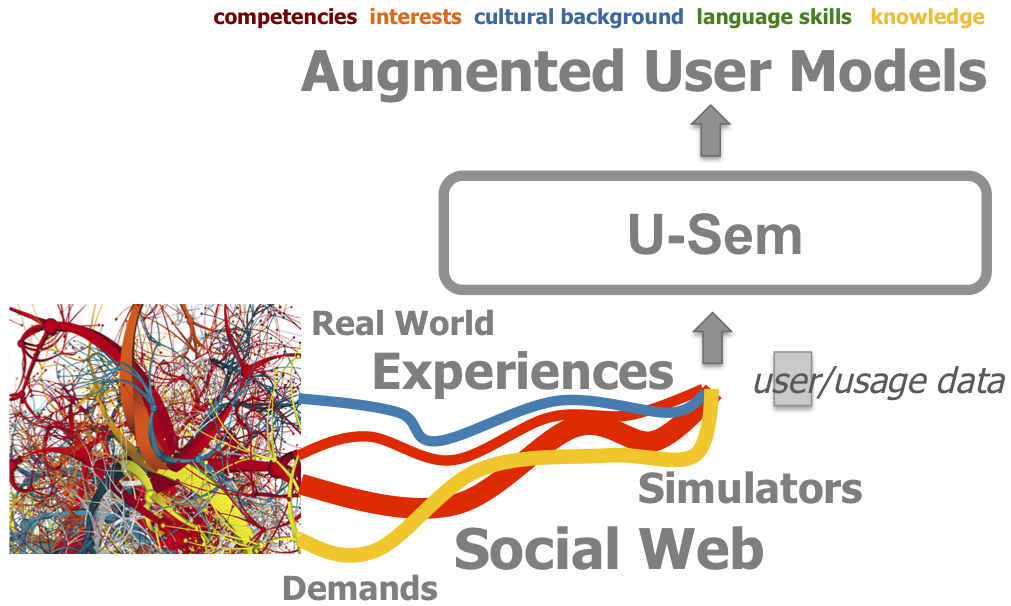
\includegraphics[width=11cm]{img/usem-logo.png}}


% A copyright notice and maybe something about the cover picture
% Put in comments to get the default copyright notice
\colophon{\noindent\copyright{} 2013 \theauthor. Coverpicture: some picture.}

% thesis committee:
\chair{Prof. dr. ir. Geert-Jan Houben, Faculty EEMCS, TUDelft}
\supervisor{Dr. ir. Jan Hidders, Faculty EEMCS, TUDelft}

% The following two are optional for LaTeX (current university regulations state that at least one of them should be assigned)

\committeemember{Dr. Andy Zaidman, Faculty EEMCS, TUDelft}
%\externalsupervisor{Ir. H.J.A.M. Geers, Faculty EEMCS, TUDelft}


\setsecnumdepth{subsection}\maxsecnumdepth{subsection}

\makeatother

\usepackage{babel}

\begin{document}
\frontmatter 

\thispagestyle{empty}

\maketitle % main title page

\makeformaltitlepages{With the increasing popularity of social media, more and more user data is published on the web everyday. As a result, there is a high demand for engineers to devise different algorithms for user modelling based on that data. The U-Sem framework defines an approach for constructing such algorithms and providing them to the customers in the form of user modelling services.

The process of building these services, however, requires engineers to perform a lot of manual tasks, many of which are not connected to the core of the engineers' specialization. These tasks are considered as significant overhead and are reported to cause poor performance of engineers. Therefore, in order to solve that problem, in this thesis we present the design and implementation of the U-Sem platform. It extends the U-Sem idea for building user modelling services by providing a platform that facilitates the work of the engineers.

Based on the analysis of the current process for building U-Sem services we solve the two problems which solutions were indicated to be the most beneficial for the engineers. The first one is to enable engineers to add and remove the functional components that build up the services to/from the platform on demand without affecting the work of others using it. While the second problem is to enable engineers to create and process the persistent data required for the services transparently without being aware of where and how it is actually stored.} % formal title pages

\cleardoublepage{}
\chapter{\label{cha:Preface}Preface}

This master thesis is the final work of my study at Delft University of Technology. As part of my part-time job for the WIS group I had to  build several U-Sem services myself which gave me the chance to personally experience the problems that scientists face every day. This helped me to generate a lot of ideas on how to improve that situation. At the end, it also gave me the confidence that my work is not just  another master thesis but it is actually something that will be used, save a lot of time and efforts to the scientists and hopefully, help them create ever grater user modelling algorithms.

I really want to take this opportunity to acknowledge all of those who have given me support and guidance during my studies. I would like to thank everyone from the WIS group and especially my supervisors Jan Hidders and Jasper Oosterman who helped me a lot with my daily struggles. And last but not definitely not least I am really grateful to Prof. Houben for all his support and for the wonderful opportunity to be part of his team.


\vskip1cm 

\begin{flushright}
\theauthor\\
 Delft, the Netherlands \\
 \today\\
 
\par\end{flushright}


\cleardoublepage{}\tableofcontents{}\cleardoublepage{}\listoffigures
\cleardoublepage{}

\mainmatter


\chapter{\label{cha:intro}Introduction}

\section{Motivation}


\subsection{Research questions}

The main research question is the following:

\textbf{How to facilitate the work of scientists and organizations interested in user modeling and analysis?}\\

The following sub-questions articulate the problem:

\begin{enumerate}
\item \textbf{How to enable users to add custom functionality and change system's behaviour?} (plug-ins)

\item \textbf{Is it possible to develop a component that enables users to store and retrieve information in arbitrary data formats?} (Universal datastore)

\item \textbf{How to enable users to maintain their results up-to-date?}  (Scheduling)


\item \textbf{How to enable multiple users to use the system simultaneously without interfering with each other and keeping their work and results protected?} (Multi User and privacy)


\item \textbf{How can real-world use cases benefit from this system?}

\end{enumerate}

\subsection{Contributions}

\subsection{Organization of the work}

There are many possible ways to approach that. One can use the waterflow model, incremental, ....

In this work we will use the incremental model because of the many advantages it brings. We design and implement one feature at a time, providing a working system after each iteration.

The last thing that has to be considered before launching the next phases of the project is to decide on the order in which the features will be implemented. This issue is addressed in the next section.

\begin{figure}[h!]
  \centering
      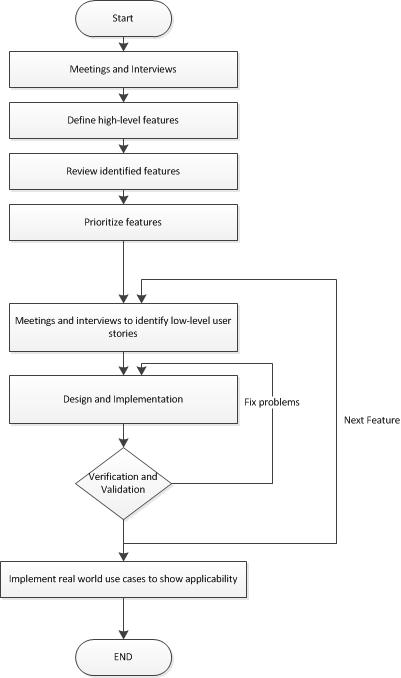
\includegraphics{introduction/WorkOrganization.jpg}
  \caption{Flow chart defining the sequence of actions taken in order to complete the project.}
\end{figure}

\subsection{Organization of the thesis}


 

\chapter{\label{cha:background}Background}
This chapter discusses the background concepts that are needed in order to articulate the problem and also the related existing works. Section \ref{sec:userModellingSystems} provides a short introduction to the field of User Modelling Systems. In Section \ref{sec:usemFrm} we briefly introduce the idea behind the U-Sem framework. Finally, Section \ref{sec:workfloManagement} presents the idea of workflow engines and elaborates on RDF Gears in particular which is currently used to support the construction of the user modelling services.

\section{User Modelling Systems}
\label{sec:userModellingSystems}

User modelling is usually considered to originate from the work of Allen, Cohen and Perrault (\cite{allen1979plan}, \cite{cohen1979elements}) and Elaine Rich (\cite{rich1979building}, \cite{rich1979user}) \cite{kobsa2001generic}. Their work had inspired many engineers and scientists to build systems that collect information about their users and adapt specifically for each them \cite{wahlster1989user}. Initially, the user modelling functionality is integrated within the systems and there is little separation between the core and the user modelling functionality \cite{kobsa2001generic}. However, in the late 80s an effort is made to decouple the user modelling functionality from the rest of the user-adaptive systems and define it as separate components that can be reused \cite{kobsa2001generic}. 

In his work \cite{kobsa2001generic} classifies the user modelling components in two categories:
\begin{itemize}
	\item \textit{User Modelling Shells} - they are part of the system that makes use of the user modelling functionality. During the development phase of the system, they have to be integrated and configured specifically for the application they are used for.
	\item \textit{User Modelling Servers} - they are not a part of the system but rather independent from it. Usually, they are "centralized", reside in the local area network or a wide area network and serve more than one applications at the same time. The main advantages of this approach lie in the fact that the information resides in a single place (no duplication and easier access control) and the functionality can be used by multiple applications which can also collaborate (information acquired by one application can be used by others).
\end{itemize}

A large number of user modelling servers have been developed over the time. Some of them are simple academic prototypes others are more sophisticated and commercially used. Examples of the foremost generic user modelling servers include DOPPELANGER \cite{orwant1994heterogeneous}, PersonisAD \cite{assad2007personisad}, Cumulate \cite{brusilovsky2004knowledgetree}, UMS \cite{kobsa2006ldap}.

However, with the increasing popularity of Social Web applications and the increasing amount of data that is published on the Web everyday there is a demand for a new type of user modelling servers that are specifically designed to take advantage of the available data on the Web \cite{brusilovsky2007adaptive}. In \cite{abel2011u} the authors address this issue and propose a special kind of framework for building user modelling servers based on various types of services. Next section discuses the idea behind it.

\section{The U-Sem framework}
\label{sec:usemFrm}

U-Sem represents a framework for semantic enrichment and mining of people's profiles from usage data on the Social Web. It provides methodology for designing services for user modelling and semantically augmenting user profiles. Its idea lies on the assumption that user modelling in today's Social Web sphere relies mainly on three types of input data \cite{abel2011u} that can be modelled in RDF format \cite{miller1998introduction}:

\begin{itemize}
	\item \textit{Observations} - usage data or events such as clicks, tagging activities, bookmarking actions or posts in social media.
	
	\item \textit{User characteristics} - explicit data provided by the users about their characteristics such as name, address, homepage, occupation, date of birth, etc.
	
	\item \textit{Domain knowledge} - this data is needed in order to produce user profiles that support certain application domains.
\end{itemize}

Based on these types of input data the authors propose that the user modelling services can be build out of various functional components. This components are classified in the following categories:

\begin{itemize}
	\item \textit{Semantic enrichment, Linkage and Alignment} - these components are responsible to process the input data. They provide functionality for aggregating and linking user data from Social Web systems like Facebook\footnote{Facebook - http://facebook.com/} and Twitter\footnote{Twitter - http://twitter.com/}, and integration and alignment of RDF data from Linked Data providers such as DBpedia\footnote{DBpedia - http://dbpedia.org/}.
	
	\item \textit{Analysis and User modelling} - components that given the enriched data from the components in the previous group perform the analysis and user modelling generating user profiles that describe interests, knowledge and other characteristics of the users.
\end{itemize}

Services are build by orchestrating these components into workflows that provide the required functionality. The process of creating and executing workflows is usually automated using workflow management systems which are discussed in the next section.

\section{Workflow Management Systems}
\label{sec:workfloManagement}

Workflow Management Systems are systems that allow a set of high level operators that all do a single well-defined specific task to be composed in a larger whole - the workflow. Depending on the desired application some systems are specifically concerned with  timing, concurrency, synchronization, data management aspects of a complex process. They may also imply special domain specific languages for defining the workflows. Literature provides a lot of examples of workflow management systems that are currently available: \textit{Taverna} \cite{hull2006taverna}, Kepler \cite{ludascher2006scientific}, RDFGears \cite{feliksik2011}, etc.

RDF Gears seems the best option for engineers applying the U-Sem framework because, firstly, it is specifically designed to deal with RDF data which is how all the user modelling inputs are modelled according to the specification of the U-Sem framework. Secondly, it is already being used by some engineers and it has proved to be suitable for the situation. In next section, we will discuss how RDF Gears works and what are its features.

\subsection{RDF Gears}
\label{sec:backRDFGears}

RDF Gears is a workflow management system designed specifically for building workflows for integration and transformation of RDF data \cite{feliksik2011}. It aims to provide a data integration framework that allows expressing and executing complex algorithms. RDF Gears consists of three main components: RDF Gears Language, RDF Gears Engine and RDF Gears graphical user interface \cite{feliksik2011}:

\paragraph{RDF Gears Language (RGL)} is a workflow language that is used to define the workflows as a combination of functional components. Each functional component has zero or more inputs and one output and defines certain operation that is performed on its inputs. The result of the operation is provided as the output of the component. The inputs are defined as input ports and can be connected with a particular output port of another component. All ports are associated with data type. The type system of the language is discussed in next subsection. The connections between the components represent the flow of data between them. Components and the connections between them form an acyclic directed graph which is the actual workflow. 

\paragraph{RDF Gears graphical user interface} represents a web application that facilitates the construction of workflows in order to make the construction of complex RGL expression easier. It provides drag and drop operation for editing worklfows and visualizing the connection between components as a visual directed graph \cite{maro2011}. The GUI builds the defined workflows as XML files which are the workflow source code that represent the RGL expressions and are executed by the RDF Gears Engine.

\paragraph{RDF Gears Engine} represents an application that is responsible for the execution of the predefined workflows by evaluating of the RGL expressions. Discussed in next subsection, it also provides optimizations for efficient execution of workflows. The engine expects as an input the XML files that define the workflows and provides graphical and RESTful interfaces that enable users to execute the workflows. 

RDF Gears also comes with a set of built-in components that can be used for creating workflows. However, this set is not exhaustive and usually engineers have to implement their custom components in order to be able to build the required user modelling services. The engine is implemented in Java and the process of adding custom components to it requires the following steps: First, engineers have to check out the source code of RDF Gears from the software repository. Then, they have to implement their components in Java and add the result Java classes and resources to the source code of the engine.  Finally, they have to build the system and deploy it on a Web Server so that is available to the users.

\subsubsection{Type System}

The RGL language defines values and type systems. The values of RGL combine the value system of the Named Nested Relational Calculus (NNRC) with the RDF data model \cite{feliksik2011}. The RGL values can be defined as follows:

\begin{itemize}
	\item Every RDF value (URI, literal or graph) is a value in RGL.
	
	\item If r is a named row over values, then [r] is a value which is called a record.
	
	\item A finite multi set of values is a value that is called a bag. Bags are restricted to contain only values of the same type.
\end{itemize}

RGL uses static type system that allows engineers to specify the expected input and output values for each component on design time. It also allows the evaluation of the RGL expression to be performed before the actual execution in order to ensure the correctness of the RGL expression. RGL introduces types for the URI, literals and RDF graph values. We refer to them as basic types. RGL types are inductively defined as follows:

\begin{itemize}
	\item The basic types are types
	\item If T is a named row over types, the Record(T) is a type that defines record values
	\item If T is a type, then Bag(T) is a type that defines bag values
\end{itemize}

\subsubsection{Optimizations}

In order to execute the predefined workflows efficiently RDFGears performs special optimizations like pipelined bag iteration, lazy evaluation of expressions and buffered, streaming serialization \cite{feliksik2011}. Designing the solution proposed in this work we have to ensure that the current way for compiling and executing workflows is not compromised and also workflows are still optimized in order to execute efficiently. 

The way RDF Gears engine applies some of the optimizations is based on the assumption that wokrlfows are build from components that have no side effects. This means that they are only responsible to produce its output value and do not change its state or the state of any other component or system. As a result, if the output value of a component is not needed the engine can decide not to execute it at all and there will be no change in the behaviour of the workflow. The engine takes advantage of this idea in two aspects:
	\begin{itemize}
		\item \textit{Wokflow compilation} - workflows are compiled into a data structure which represents directed graph and contains the output node and all components that the output directly or indirectly depends on. Therefore, if there is no path in the graph from a component to the output node then the component is removed. The removed components are never executed.
		
		\item \textit{Workflow evaluation} - the engine provides functionality that performs lazy evaluation of the compiled workflows. The engine takes the output node and recursively executes all components which outputs are needed for the execution. As a result, components which output is not requested are not executed at all (eg. when the If/Then/Else component is used). Additionally, when a component's output is required by several components then the first time it is executed it cashes its result value and directly provides it for the next request. Therefore, RDF Gears guarantees that each component is executed at most once.
\end{itemize}


\chapter{Problem definition}
\label{cha:problemDef}

In this section we define the problems that have to be solved in order to reach our research goal. Section \ref{sec:mainProblem} presents the high level problem and shows the process we followed in order to identify the features that the system has to provide in order to solve that problem. In Sections \ref{sec:problemDefPlugin} and \ref{sec:problemDefStorage} we identify the sub-problems connected to each of the features. 

\section{High-level Problem}
\label{sec:mainProblem}

As discussed in Section \ref{sec:usemFrm}, the U-Sem paradigm defines how user modelling services are constructed by orchestrating specific types of functional components. It does not, however, provide any formal mechanism or guidelines about how these services and components are constructed and managed in practice. Currently, the only work done in that direction is the adoption of a workflow management system (RDF Gears) which facilitates the orchestration of components into user modelling services. 

Discovering the potential of Social media for user modelling \cite{brusilovsky2007adaptive} has led to an increased demand for U-Sem engineers to design and build many different user modelling services. As a result, engineers are constantly required to implement or adapt variety of functional components that are needed for the new services. Currently, there is a lack of standardized approach and tools that support this process and as a result it requires a lot of manual work and is not efficient. Because of the high demand for user modelling services, the deficiencies in the process have a big negative impact. Our investigation showed that this causes a lot of disturbances and reduced performance to the engineers. Therefore, in this work we investigate whether the current situation can be improved by introducing a user modelling server that is designed to facilitate the process of creating and exposing the user modelling services to the users so that the overhead work of the engineers is limited and they can focus on the core of their work - the user modelling and analysis algorithms.

In order to be able to provide such system we, first, have to identify how engineers work and what are the tasks that require them to do a lot of overhead work and can be potentially fully or partially automated. This is covered in next section.

\section{Overhead tasks}

The task of identifying these overhead tasks is a form of requirements gathering \cite{hickey2004unified} and thus, we investigated the literature to find a suitable approach for doing it. There is a wide variety of possible approaches for requirements gathering \cite{hickey2004unified} : interviews, questionnaires, user observation, workshops, brain storming, role playing, etc. We decided to use the semi-structured interviews technique since it is widely used and it has proved to be effective through the years \cite{dieste2008understanding}.

In order to perform the interviews we first have to identify the stakeholders. Stakeholders are the people that have some kind of interest in the project. They are the ones that will be affected by the project and thus they are the source for identifying the characteristics of the system we have to build. In our case the main stakeholders are the engineers that are already using or will use the U-Sem approach for constructing user modelling services. 

Having identified the target people we performed the interviews, the results of which are summarized in the next section. 

\subsection{Identified overhead tasks}
\label{sec:features}

We carefully analysed all the raw information that was gathered from the interviews and we identified several tasks that require engineers to do a lot of overhead work. We presented them to the stakeholders and after some discussions we ended up with the following final list: 

\begin{itemize}

\item \textbf{Access to social media}
Engineers base a lot of their analysis on the information provided by users in the social media. However, each social media web site provides access through a special API. Currently, each engineer has to implement a component for retrieving the required data from each type of social media he uses. Engineers report that this require them to invest considerable time and efforts.

\item \textbf{Plug in functional components}
The nature of engineers' work is very dynamic. They are constantly required to build new and improve and adapt existing user modelling services. In order to do that they usually have to create and plug into the system new RDF Gears functions and other functional components. Currently this process is done manually and represents major overhead for the engineers.

\item \textbf{Data management} 
Many of the engineers build services that need to store various types of data(e.g. intermediate and final results). Currently, they are forced to manually set-up databases and program the components needed for interacting with each type of data. This is usually not a trivial task, it requires time and knowledge and therefore, it resembles a big overhead to the engineers.

 
\item \textbf{Integration with Hadoop}
The amount of information that has to be processed in the system can sometimes be huge. Therefore, sometimes, it has to be processed by external Hadoop based systems. Currently, engineers have to manually manage the exchange the information to and from the Hadoop systems.

\item \textbf{Scheduled execution of services}
Some services require to be executed on regular bases. For example, a service that has to monitor how certain user profile changes over time might need to be executed daily. Currently, this execution has to be manually accommodated by the engineers and it becomes a serious overhead when they are responsible for many services like that. 

\end{itemize}

Having identified the tasks that engineers find most problematic allows us to rephrase our goal into providing a solution that is designed to facilitate these tasks. Facilitating each of these tasks is a feature that the system has to provide. The limited scope of this thesis work, however, does not allow us to cover all of the these features and therefore, we are focusing only on providing the features that will bring the most advantage for the engineers. In order to do that, we have to prioritize them based on the impact they will provide. 

\subsection{Features prioritization}

Prioritizing the features is not a trivial task because each of the stakeholders has a slightly different view on the benefits provided by each of the features that we already identified. Therefore, we performed a research in order to find a suitable approach for dealing with this situation.

Requirements prioritization is a relatively old research topic and there are numerous approaches that are currently available \cite{moisiadis2002fundamentals}. The most popular include Quality Function Deployment (QFD) \cite{chan2002quality}, the Analytical Hierarchy Process(AHP) \cite{roper1990analytic} , as well as a variety of industrial practices such as team voting \cite{moisiadis2002fundamentals}, etc. However, literature also suggests that there is no perfect solution for this problem and the applicability of each approach depends greatly on the particular situation it is used in.

For our project, we choose the analytic hierarchy process approach \cite{roper1990analytic}. This decision was based on the fact that it is especially suitable for prioritizing a small number of requirements\cite{karlsson1997cost} and it is a proven and widely used \cite{karlsson1998evaluation}. In literature, as a disadvantage of this approach is considered the fact that it takes no account of interdependencies between requirements \cite{roper1990analytic}. However, this issue is not a problem for our solution because the project's high-level features that we want to prioritize are loosely coupled and they have little dependency between each other. 


\subsubsection{Features prioritization using AHP}
In the Section \ref{sec:features} we identified five high-level requirements(features) that cover the main functionality of the system. In this step we are using the AHP's pairwise comparison method in order to assess the relative value of each of them. It basically requires the stakeholders to systematically evaluate the importance of each of the features by comparing them to one another two at a time. Then, the AHP converts these evaluations to numerical values which represent the priority of each of the features. In order to perform this process, we instructed the stakeholders on the process and asked them to perform the evaluations by filling in a specially prepared form which is presented in Appendix \ref{cha:priority}.

We let the participants to work alone, defining their own pace. We also allowed them to choose the order of the pair's comparison. Discussions were also allowed. When all participant finished the pairwise comparison, as advised in \cite{karlsson1997cost} we had to make sure that the provided results are consistent. In order to do that we had to calculate the the consistency indices of the pairwise comparisons. According to \cite{karlsson1997cost} values lower than 0.10 are considered acceptable and even values around .12 are commonly achieved in the industry and can also be considered acceptable. The calculation showed that two of the participants have indices higher than .23 which indicates serious inconsistencies (table \ref{tbl:reqInitialConsist}). Therefore, we asked them to revise their answers and the results afterwards measured values that are acceptable (table \ref{tbl:reqFinalConsist}).
 
 \begin{table}[h!]
  \begin{center}
    \begin{tabular}{| l | l | l | l | l |}
    \hline
    & Stakeholder 1 & Stakeholder 2 & Stakeholder 3 & Stakeholder 4 \\	 \hline
    Consistency ratio & 0.04 & 0.23 & 0.13 & 0.26 \\
    \hline
    \end{tabular}
  \end{center}
  \caption{The initial consistency ratios for each of the stakeholders.}
  \label{tbl:reqInitialConsist}
\end{table}


 \begin{table}[h!]
  \begin{center}
    \begin{tabular}{| l | l | l | l | l |}
    \hline
    & Stakeholder 1 & Stakeholder 2 & Stakeholder 3 & Stakeholder 4 \\	 \hline
    Consistency ratio & 0.04 & 0.12 & 0.13 & 0.11 \\
    \hline
    \end{tabular}
  \end{center}
  \caption{Consistency ratios for each of the stakeholders after refinement.}
  \label{tbl:reqFinalConsist}
\end{table}

Once we had achieved satisfying results we calculated the distributions and outlined the candidate requirements in a diagram (Figure \ref{fig:reqPriority}). Each requirement's determined value is relative and based on a ratio scale. Therefore, a requirement whose value is calculated as 0.20 is twice as valuable as a requirement with a value of 0.10. Additionally, the sum of the values for all requirements equals 1. This means that a requirement with a value of 0.10 provides 10 percent of the value of all the requirements.

\begin{figure}[h!]
  \centering
      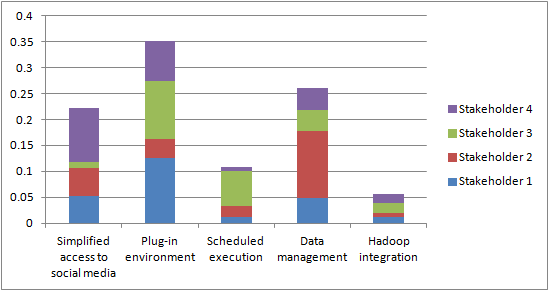
\includegraphics{requirements/value_diagram.png}
  \caption{The value distribution of the 5 requirements in the U-Sem project.}
  \label{fig:reqPriority}
\end{figure}


Finally, based on the provided results from the prioritization and because of the limited scope of this thesis we decided to design and implement the two features that will provide the most benefits for the users: "Plug-in Environment" and "Data Management". Next sections cover in details the problems connected to each of the two features.

\section{Plug-in Environment}
\label{sec:problemDefPlugin}

During the initial interviews with the engineers that are going to potentially use the system, we uncovered that the nature of their job is very dynamic. In their day to day work they are expected to constantly improve and come up with new user modelling services. As a result, they are continuously producing new software code that implements the new functional components that are needed for building the services. After each production cycle, the program code has to be deployed into U-Sem so that it is available for testing, demonstration and evaluation purposes. Currently, this process is mostly done manually by engineers who claim that it takes them a lot of time, efforts and is a source of problems that are hard to find. Therefore, the problem that we have to solve is to design a solution that facilitates this process. 

In order to be able to fully understand the problem we, first, have to fully understand how this process is currently performed. Therefore, we performed additional interviews with the engineers which showed that currently engineers follow the following process: First, they check out the latest source code of the wokrflow engine (RDF Gears) system from the source code repository and import it in their Eclipse IDE. Then, they extend it by adding the source code and other resources required for the new functional components that they build. Afterwords, they have to build and deploy the system to a web server to make it available for testing. If not satisfied with the end result, engineers apply the necessary changes and follow the build, deployment and test steps again. At the end, they have to commit the new version of the system back to the source code repository.

Analysing this process we concluded that it is far from optimal, it is error prone and it can bring a lot of discomfort to the engineers working with the system. The reasons behind this statement and also the sub-problems that have to be solved by the solution are the following:

\begin{itemize}

	\item The process requires a lot of time and efforts from the engineers engineers because it involves many tasks that are considered as overhead by engineers since they are not part of the core of their work and have to be repeated every time a functional component is added to the system.
	
	\item The deployment step of the process requires engineers to restart the web server where the system is deployed. As a result, during the time the server is down all other running services are unavailable. This is a major problem for everyone that is using the system during that time.
	
	\item Another serious problem comes from the fact that every step of the process requires engineers to have certain kind of knowledge in order to be able to perform it. As a result, the training period for new engineers is significantly increased. This may easily cause project delays and missed deadlines.
	
	\item Multiple engineers performing the process simultaneously may result in loss of functionality. Figure \ref{fig_vers_prob} illustrates the problematic scenario. As stated earlier, in order to add new functionality, engineers must first check out the source code of the system, make the changes and deploy the new version on the web server. However, if two engineer perform this process simultaneously then the new functionality provided by the first engineer will be lost when the second one deploys his version. 
	
	\begin{figure}[h!]
  \centering
  	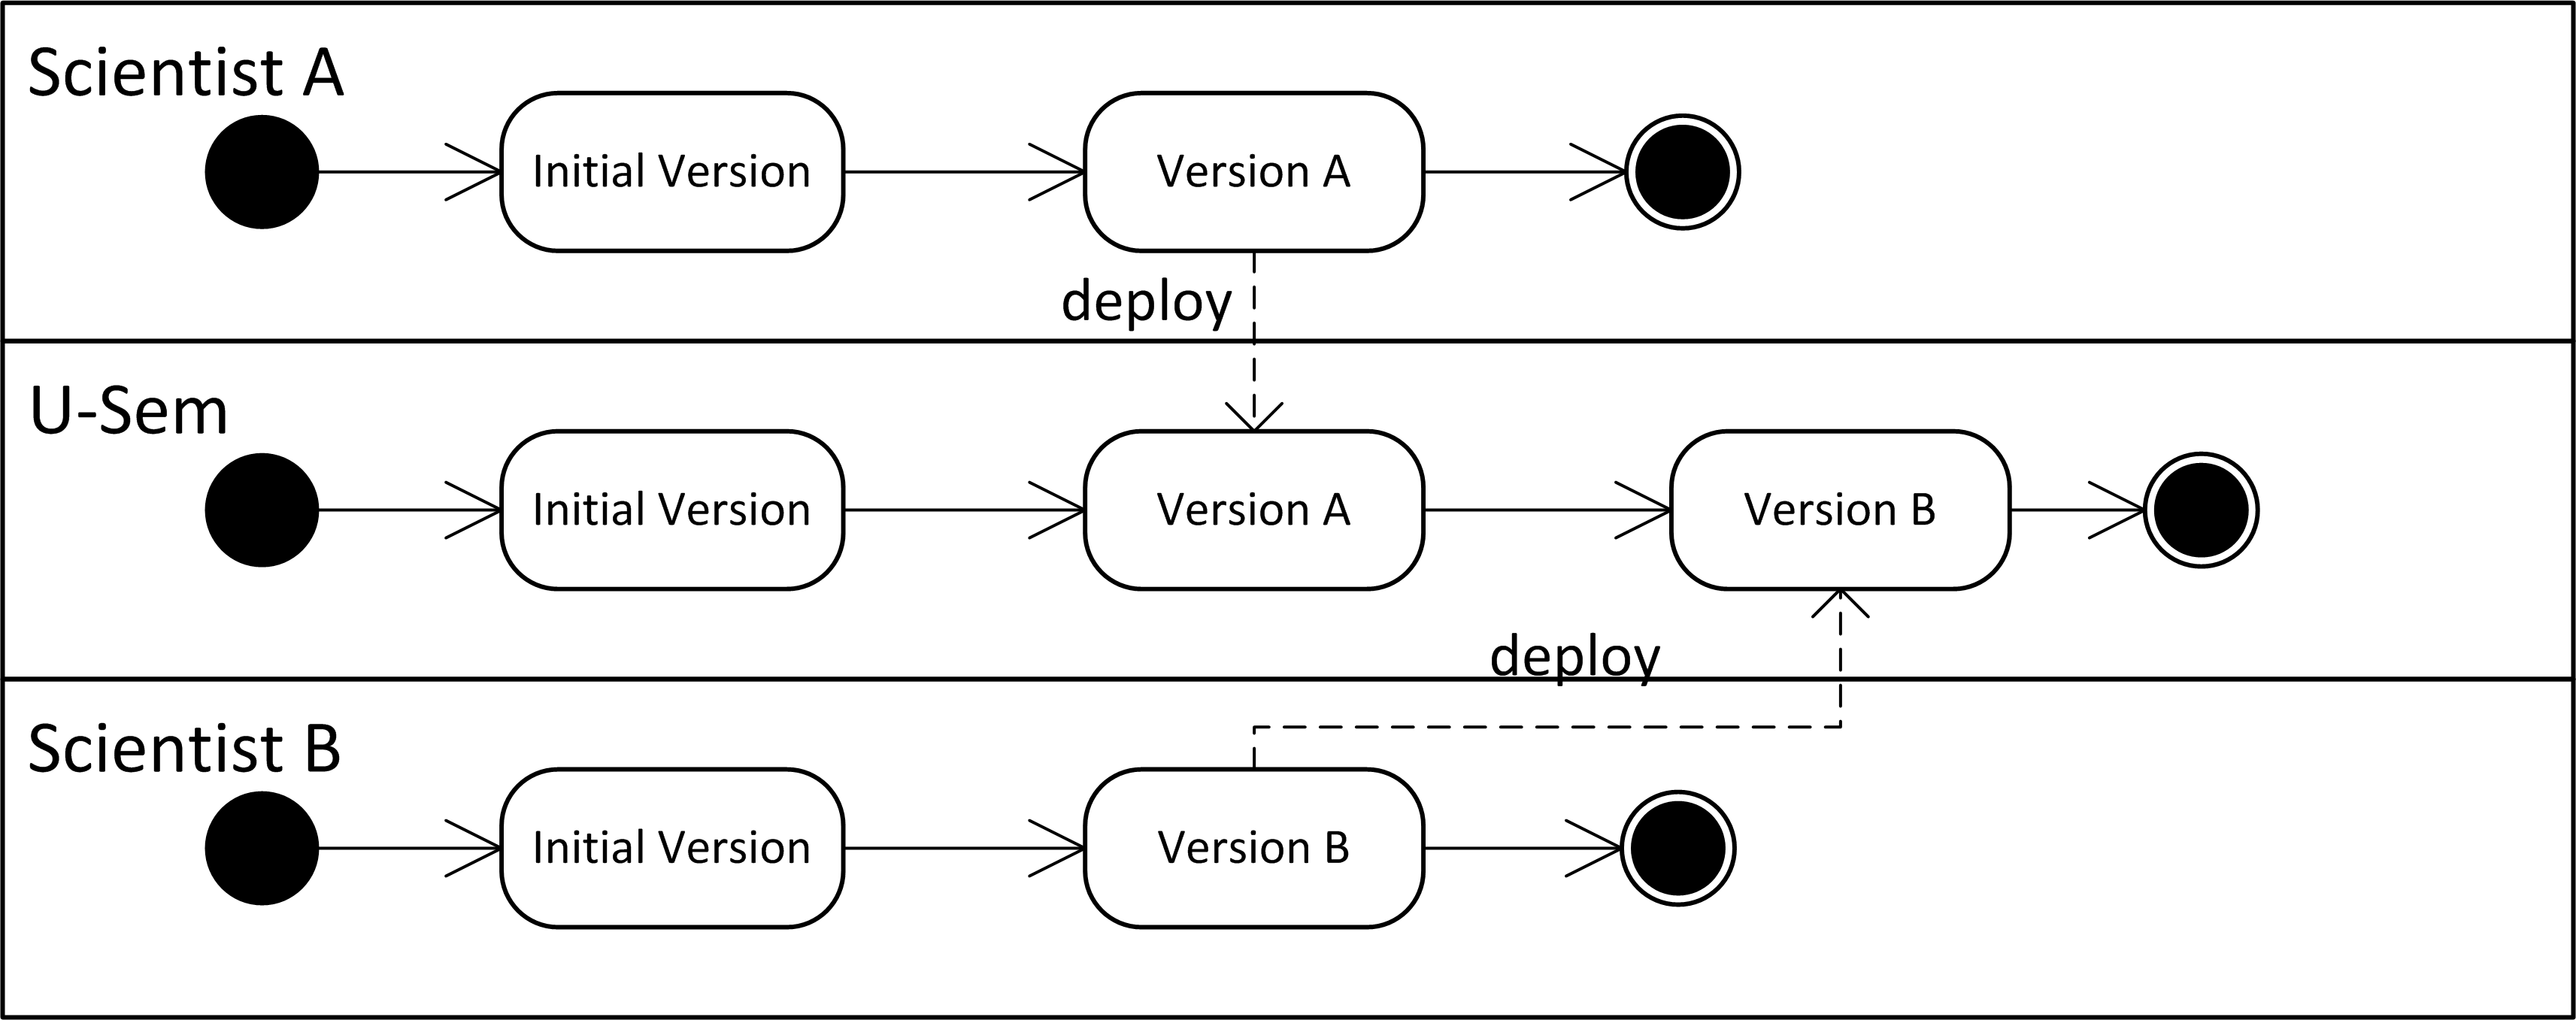
\includegraphics[scale=0.75]{plug-in/version_problem.png}
  \caption{State diagram illustrating the scenario where two engineers extend U-Sem simultaneously and the changes made by engineer A are lost.  }
  \label{fig_vers_prob}
\end{figure}
	
	\item Engineers also reported that following the current process the source code implementing the different functional components resides in the same project and as a result, they have become, over time, tightly coupled between each other. This has made them very hard to be maintained and extended.
		
\end{itemize}

We believe that providing a solution that overcomes these problems will significantly improve the current situation enabling engineers to focus more on the core of their work. In next section, we cover the "Data Management" issue and identify the problems hiding behind it.


\section{Data Management}
\label{sec:problemDefStorage}

The interviews that we performed with the engineers showed that many of the services they implement require functional components that provide means for executing data storage and retrieval operations. They reported that the structure and semantics of the data and the particular operations they have to perform on it varies a lot but the main scenarios can be classified in the following groups:

\begin{itemize}

	\item \textit{Raw data} - Engineers reported that most of the modelling services they build are based on the social media. Basically, they have to retrieve certain entries (e.g tweets from Twitter ) which are the basis for the user modelling. In certain cases engineers have to store this "raw data" locally. Usually, this is as a result of the fact that retrieving the entities from the social media web sites is time consuming and also some of the APIs limit the number of entities one can get for a certain amount of time \cite{cheong2009integrating}. This makes the execution of workflows slow because the system has to wait to get the needed entries every time. Therefore, engineers are forced to store these entries locally and only make sure they are up-to-date prior to the execution of a workflow.
	
	\item \textit{User provided data} - Some services require information that is not available from social media and has to be provided by the users of the system. For example, in certain use-cases users have to fill in questioners so that the results from future user modelling are adjusted based on the answers provided by the users. It is infeasible to ask the users for that information every time the service is executed and that is why it has to be stored within the system.
	
	\item \textit{Intermediate results} - Some services consist of two phases. The first phase continuously calculates some intermediate representation of the raw data. In the second phase, on user request the final result is calculated based on the intermediate data. One such example is the Twinder service \cite{tao2012twinder}. Therefore, between the two phases, the intermediate results have to be stored and later retrieved back.
	
	\item \textit{User profiles} - Some services require that users are able to monitor how the generated user profiles evolve over time. For example, in e-learning systems users want to be able to see how the knowledge of a certain person has changed after following a certain course in order to measure how helpful the course was for that person. Therefore, every time a service is executed the results have to be stored so that they can be further analysed later.
	
	\item \textit{System data} - Finally, many of the features of the system need to store some kind of information. For example, the user authentication functionality has to store all kind information about the users of the system: user names, passwords, privileges, etc. The scheduling feature has to store information about the time at which each service has to be executed. 
	
\end{itemize}

Clearly, there are a lot of scenarios that require data storage and retrieval operations and currently, the system does not provide any means to support engineers in defining workflows that require such operations. Each engineer is responsible to set up a database server and create custom RDF Gears components that serve the particular needs. However, this process requires a lot of time and efforts, and suffers from many downsides and problems:

\begin{itemize}
	\item \textit{Knowledge required} - designing and implementing components for dealing with persistent data is not a trivial job and requires specific type of knowledge. Many of the engineers building services have mathematical or statistical backgrounds and are likely not to have in depth knowledge in the database field. In order to be able to build their services they have to acquire this knowledge which can cause significant overhead and waste of time. Additionally, the fact that they are not professionals in the field may lead to problems and shortcomings.
	
	\item \textit{Server administration} - Most of the storage solutions require setting up a dedicated database server. These servers have to be hosted somewhere, maintained, backuped, etc. All these tasks require a lot of effort and if every user has to do it, it will result in large amount of duplicated work and overhead. If engineers decide to use a shared database server then appears the question of who is responsible to manage it and ensure its security and privacy.
	
	\item \textit{Dynamic data structure} - It is expected that the structure of the stored data might change over time. When a database with fixed schema is used (like most SQL solutions) then every time the structure changes the engineers have to connect to the database and apply the changes manually. This task is likely to be annoying, time consuming and even error prone for some engineers. Therefore, automating this process can save time to engineers and reduce the number of mistakes caused by carelessness. 
	
	\item \textit{Collaboration} - collaborations between engineers on data level is reported to be quite important and can save them a lot of time. Currently, there are no facilities available to support that requirement. Engineers have to organize this collaborations personally. Additionally, because the collaborations are not integrated in the system they are likely to be hard to monitor and control.
	
	\item \textit{RGL translation} - Generally available database solutions are not capable to deal with data in the RGL format introduced in RDF Gears. Therefore, every single component that deals with persistent data has to translate the RGL values to values compatible with the database solution and vice versa. Clearly, all this code is redundant and removing this responsibility from the engineers will save them time and efforts so that they can focus their attention to the core of their work.
	
	\item \textit{RDF Gears and components with side effects} - Components that store data are components that have side affects. However, as discussed in Section \ref{sec:backRDFGears} RDF Gears is not designed to work with such components and some unexpected behaviour might be expected. Therefore, engineers building components with side effects that are not aware of the way RDF Gears operate internally risk to introduce problems that may be also hard to detect.
	
\end{itemize}

In this thesis we aim to propose a solution that is capable to overcome these problems and save engineers a lot of time, efforts and prevent mistakes while dealing with persistent data.

\section{Conclusion}

In this chapter we identified the problems that we have to overcome in order to achieve our research goal. In order to do that we conducted series of interviews and identified the features that have to be provided by the system. We evaluated the importance of each of the them and chose to focus our work on the two areas which were indicated to be most beneficial for the engineers: "Plug-in environment" and "Data Management". We further investigated both of them in order to identify the sub-problems that have to be solved for each of them. Next chapters are dedicated to each of the two areas and present the architecture and implementation that we propose in order to solve the identified problems. Chapter \ref{cha:plug-in} covers the Plug-in environment and Chapter \ref{cha:data} is dedicated to the Data Management feature. 

\chapter{Plug-in Environment}
\label{cha:plug-in}

This chapter presents the design and implementation of the "Plug-in Environment" feature of the U-Sem platform. Section \ref{sec:requirementsPlugin} identifies all functional and non-functional requirements that a successful solution must satisfy based on the problems discussed in Section \ref{sec:problemDefPlugin}. Section \ref{sec:approachPlugin} discusses the state of the art approaches and technologies that can contribute to solving the problem. Section \ref{sec:architecturePlugin} describes the architecture that we propose in order to solve the problem. In Section \ref{sec:implPlugin} we discuss the implementation that we provide in order to be able to verify the capabilities of the proposed architecture. Section \ref{sec:evalPlugin} evaluates whether the proposed solution solves all of the defined problems. Finally, in section \ref{sec:limitsPlugin} we discuss the limitations of the proposed design and suggest aspects in which the solution can be improved in the future.

\section{Requirements}
\label{sec:requirementsPlugin}

Having identified all the problems concerning the feature in section \ref{sec:problemDefPlugin}, we propose a solution that is based on the following idea: Engineers wrap the new RDF Gears functions and the required additional resources they develop into components. These components are build and maintained independently from the workflow engine. Engineers are able to install the components to the system when they want to use them.

Following this idea we devised a set of requirements that presents the functional scenarios (functional requirements) and system qualities (non-functional requirements) that the proposed architecture has to provide.

\subsection{Functional Scenarios}
In this section we formally identify the functional requirements which define the main interactions between the engineers and the system. Each scenario is marked with a code at the beginning which is used for easier identification during the verification and evaluation phase.

\begin{itemize}

	\item \textbf{UC1 - Create components for U-Sem} - Engineers have to be able to compose the functionality they produce (mainly RDF Gears functions and the required additional resources) into components that can be plugged into U-Sem when the functionality is needed.
	
	\item \textbf{UC2 - Install components to U-Sem} - Engineers have to be able to extend U-Sem by adding components on demand without having to restart the system and affecting the work of other engineers using the system.
	
	\item \textbf{UC3 - Sharing components} - Since the new functionality provided by engineers is no longer part of the system other engineers do not have direct access to it. Therefore, the system has to enable engineers to share components and use the ones shared by others.
	
	\item \textbf{UC4 - Manage installed components} - Engineers have to able to manage all components already added to the system. This includes, firstly, that they have to be able to view a list of all installed components. And secondly, they have to be able to remove any of them.
			
\end{itemize}

\subsection{Non-functional requirements}

This section identifies the main quality scenarios that a successful architecture has to accommodate. 

\begin{itemize}
	
	\item \textit{Isolation} - Any engineer should not be affected by the work of the others. The only way of interaction between engineers has to be achieved through the component sharing mechanism. Furthermore, engineers should not be affected by any future changes to the reused components.
		
	\item \textit{Security} - This is also very important requirement since the system executes custom code and thus, is vulnerable to deliberate or unintentional exploitation of vulnerabilities. Therefore, the system should provide mechanism that enables administrators to enforce different restrictions on the executed custom code. For example, the administrators might want to forbid engineers from accessing the file system or the network.
	
\end{itemize}

\section{Approach}
\label{sec:approachPlugin}

This section discusses the approach that we propose for designing the "Plug-in Environment" feature of the U-Sem platform. After carefully analysing the requirements specified in the previous section we identified four steps that have to be followed in order to provide the desired solution:

\begin{itemize}
	\item \textit{Modularization and component management} - define how the system is modularized into components that can be added and removed from the system on demand without affecting its operation.
	\item \textit{Collaboration between engineers} - enable engineers to collaborate and reuse each others work.
	\item \textit{Dependencies management} - help engineers to manage the dependencies between components ensuring that the system is in a consistent state.
	\item \textit{Component construction support} - assist and if possible automate the process of creating components.
\end{itemize}

Next subsections address each of these steps presenting the way they are approached and performed. 

\subsection{Modularization and component management}
\label{sec:pluginModulAndManag}

We investigated the scientific literature to find what are the available approaches and technologies that we can take advantage of in this step. Our research revealed that the topic about modularization of software systems is widely discussed and there is even a sub field in software engineering which addresses the problem of building systems out of different components: \textit{Component-based software engineering}  \cite{jifeng2005component}. In this section we discuss the basic idea and the advantages that it brings. We also discus what features a system needs to provide in order to enable Component-based software engineering. This is known as component model. At the end, we present the component model implementation that is to be used in the design and implementation of the system. 

\subsubsection{Component-based software engineering}

Component-based software engineering is based on the idea to construct software systems by selecting appropriate off-the-shelf components and then, assemble them together with a well-defined software architecture \cite{pour1998component}. This software development approach improves on the traditional approach (building an application as a single entity) since applications no longer have to be implemented from scratch. Each component can be developed by different developers using different IDEs, languages and different platforms. This can be shown in Figure \ref{fig_cbsd}, where components can be checked out from a component repository, and assembled into the desired software system. This completely complies with the idea behind U-Sem where each engineers is responsible to build only a peace of the system which provides certain service.

\begin{figure}[h!]
  \centering
  	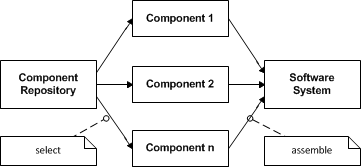
\includegraphics[scale=0.75]{plug-in/component-based.png}
  \caption{Component-based software development \cite{pour1998component} }
  \label{fig_cbsd}
\end{figure}

Other benefits that Component-based software development brings and we believe U-Sem will benefit from include: significant reduction of development cost and also improvement on maintainability, reliability and overall qualities of software systems \cite{pour1999enterprise} \cite{pour1999making}. Additionally, the applicability of this approach is supported by the fact that it is widely used in both the research community and in the software industry. There are many examples of technologies implementing this approach including: OMG's CORBA \cite{vinoski1997corba},  Microsoft's Component Object Model (COM) and Distributed COM (DCOM) \cite{sessions1997and}, Sun's(now Oracle) JavaBeans and Enterprise JavaBeans \cite{goncalves2010enterprise}, OSGi \cite{tavares2008gentle}.


\subsubsection{Component model}

Designing the component model of a system provides the specification defining the way that the system can be build by composing different components applying the component-based software engineering approach. More formally, it is the architecture of a system or part of a system that is built by combining different components \cite{cai2000component}. It defines a set of  standards for component implementation, documentation and deployment. Usually, the main components that a component-based software system consists of are \cite{chen2009refinement}:

\paragraph{Interfaces}
	determine the external behaviour and features of the components and allow the components to be used as a black box. They provide the contract which defines the means of communication between components. As illustrated on Figure \ref{fig_intf}, interfaces can be considered as points where custom functionality provided by another component can be plugged in. 
	
	\begin{figure}[h!]
  		\centering
  		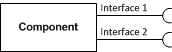
\includegraphics[scale=0.75]{plug-in/component-interfaces.png}
  		\caption{Component interfaces }
  		\label{fig_intf}
	\end{figure}

\paragraph{Components}
	are functional units providing functionality by implementing interfaces. As can be seen on Figure \ref{fig_comp}, components provide  features by implementing the interfaces provided by other components. One of the main question regarding building components is how to define the scope and characteristics for a component. According to \cite{cai2000component} there are no clear and well established standards or guidelines that define this. In general, however, a component has three main features: 

\begin{itemize}
	\item a component is an independent and replaceable part of a system that fulfils a clear function
	\item a component works in the context of a well-defined architecture
	\item a component communicates with other components by its interfaces 
\end{itemize}

	\begin{figure}[h!]
  		\centering
  		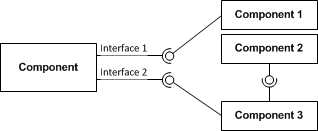
\includegraphics[scale=0.75]{plug-in/component-services.png}
  		\caption{Components implementing interfaces }
  		\label{fig_comp}
	\end{figure}

\paragraph{Coordinator}
	is the entity which is responsible to glue together and manage all the components. It is needed because components provide a number of features, but they are not able to activate the functionality themselves. This is the responsibility of the coordinator.

\subsubsection{Component model implementation}

In previous sections, we discussed that integrating a component model in the architecture of U-Sem is the scientifically proven approach that promises to solve the design problem and fulfil the requirements of the customers. However, we had to decide whether to design and implement our own custom component model or we can reuse an existing one. Reusing a popular and widely used solution might be beneficial because it is likely that it is well tested (at least from the engineers using it) and thus provide higher quality. 

\cite{lau2007software} suggests classification of the component model implementations based on which part of the life cycle of a system the composition of the components is done. They identify the following groups:

\begin{itemize}
	\item  Composition happens during the design phase of the system. Components are designed and implemented in the source code of the system.
	\item  Composition happens during the deployment phase. Components are constructed separately and are deployed together into the target execution environment in order to form the system.
	\item Composition happens during the runtime phase. Components are put together and executed in the running system.
\end{itemize}

For the architecture of U-Sem we are only interested in the last group since one of the main requirements is that engineers should be able to add, update and remove components while the system is running, without restarting it. This is essential since the system is used by multiple engineers and system restart will cause temporary unavailability of all services. 

Apart form this, there is also another critical concern when choosing component model implementation for U-Sem. The implementation should support the Java language since it is the language in which all current services are implemented and most engineers are familiar with. Having to learn a new language and/or rewriting all source code in different language is considered as a big disadvantage for the engineers.

We performed further investigation in order to find what are the current state of the art technologies that satisfy all requirements. It showed that currently there are two standards that satisfy our needs: Fractal \cite{bruneton2006fractal} and Open Services Gateway initiative (OSGi)\footnote{OSGi Alliance - http://www.OSGi.org}. Both of them seemed quite popular and widely used and therefore we concluded that reusing one of them is more beneficial than implementing a component model from scratch. For the proposed architecture of U-Sem we chose to use OSGi since our impression is that it provides a simpler way of defining components (no component hierarchies) which will be beneficial for engineers that do not have so in-depth knowledge of component-based engineering. OSGi is also widely used \cite{tavares2008gentle} which may suggest that it is well tested and therefore is more stable. Next subsection focuses on how OSGi works and its features that are interesting for the architecture of U-Sem.


\subsubsection{OSGi}

Proposed first in 1998, OSGi represents a set of specifications that define a component model which represents a dynamic component system for Java. These specifications enable a development model where applications are dynamically composed of different independent components. Components can be loaded, updated and deleted on demand without having to restart the system. OSGi defines the main components of the standard component model which are discussed in the previous section as follows:

\begin{figure}[h!]
  \centering
  	\includegraphics[scale=0.6]{plug-in/OSGi.png}
  \caption{OSGi Service Registry \cite{tavares2008gentle}}
  \label{fig_OSGi}
\end{figure}

\paragraph{Interfaces}
 in OSGi define the contract for communication between different components by describing the operations that have to be implemented by them. Basically, they represent standard Java interfaces or classes which have to be available to both the component that implements the interface and the components that use the implemented functionality.


\paragraph{Components}
  in OSGi are called bundles. Bundles are basically a regular Java JAR files that contain class files and other resources such as images, icons, required libraries. One of the important benefits for U-Sem is that OSGi enables better modularization providing facilities for better information hiding then the one provided by the Java language \cite{tavares2008gentle}. Each bundle should provide a manifest file, which enables engineers to declare static information about the packages that are exported and therefore can be used by other bundles. Furthermore, bundles provide functionality to the rest of the system in the form of services. In the OSGi architecture, services are standard Java objects that implement the interfaces described in the previous paragraph. Note that in the reminder of this chapter we will also refer to the OSGi bundles as \textit{plug-ins}.

\paragraph{Coordinator}
The OSGi standard also provides coordinator component which represents a runtime infrastructure for controlling the life cycle of the bundles which includes adding, removing and replacing bundles at run-time, while preserving the relations and dependencies among them. Another key functionality that the coordinator component of OSGi provides is the management of the services provided by the bundles. This functionality is provided by the Service Registry, which keeps track of the services registered within the framework. As illustrated on Figure \ref{fig_OSGi}, when a bundle is loaded it registers all the services that it implements (step 1). As soon as a service is registered, it can be retrieved by any other components that are interested in this functionality (step 2). Once a bundle has retrieved a service, it can invoke any method described by the interface of this service (step 3). Another interesting feature of the OSGi Service Registry is its dynamic nature. As soon as a one bundle publishes a service that another bundle is interested in, the registry will bind these two bundles. This feature is very important for U-Sem since it will enable engineers to plug in any new functionality dynamically when it is needed.

\subsubsection{Security}

The security capabilities of OSGi are also very important for U-Sem since a lot of custom code is being executed which poses a significant threat to the system. The OSGi platform is considered to be highly secure by its creators \cite{parrend2009security}. There are two main reasons in favour of this statement. Firstly, OSGi is executed on top of the JVM and inherits its security capabilities. Secondly, it has been designed to support a proper level of isolation between components.

Since its introduction, the Java language and JVM have been widely used and subjected to extensive tests and validation \cite{parrend2009security}. The platform was designed to support the safe execution of fully untrusted code \cite{dean1996java}. In order to achieve this, it has introduced the following features \cite{gong2003inside}: Type Safety of the language, Garbage Collection (no user-defined memory management), Bytecode verification ensuring that executed programs are compliant with the language specification, and Sandboxing, which can prevent the access to sensible resources like the network or file system. Additionally, the system provides secure class loaders, which enable loading of several modules that cannot interact with each other.

On top of this, OSGi defines additional permissions that provides full control of the interactions between the components. It provides functionality that enables dependencies at package level and at the service level to be allowed or prevented. Additionally, bundle management capabilities of one component to the others can also be restricted \cite{parrend2009security}.

\subsection{Collaboration between engineers}

Engineers have to be able to collaborate between each other by reusing each others functionality. In order to support this feature we propose an approach based on the \textit{Component Repository} idea \cite{seacord1999software}. We introduce a plug-in repository which represents a storage location where plug-ins are stored and when needed, they can be retrieved and installed into the system. When engineers build a new plug-in then they can share it with other engineers by publishing it at the repository so that anyone interested can install and use it. The applicability of this approach is also supported by the fact that it is used in other plug-in based systems like Eclipse \cite{mcaffer2010eclipse} as well.

Using the plug-in repository engineers are able to exchange plug-ins before they are installed into U-Sem. An alternative approach is to enable engineers to share already installed plug-ins between each other. In this way, whenever an engineer creates a new version or an entirely new plug-in it is installed to U-Sem, shared and then all other engineers are able to use it. However, that approach has one major disadvantage. When a new version of a plug-in is installed then all engineers automatically start to use the new version. The version, though, might introduce a bug or it might not be completely compatible with the previous version. As a result, all other engineers' services and plug-ins that are using it are threatened to experience failures. 

Using the Plug-in repository overcomes this problem. When an engineer releases new version of a plug-in, other engineers can decide whether or not to immediately adopt the new release. If they decide not to, they can simply continue using the old one. Later, when they decide that are ready for the change, they install and use the new release. The benefit from this approach is that none of the engineers are at the mercy of the others. Changes made to one plug-in do not have an immediate affect on other engineers that are using it. Each engineer can decide whether or when to move to the new releases of the plug-ins in use.

\subsection{Dependencies management}

It is very likely that plug-ins have dependencies between each other. This may be as a result of reusing functionality from other engineer's plug-ins or depending on a plug-in that provides common functionality like extracting data from social media and storing data into a database. In order to use such plug-in engineers have to make sure that all its dependent plug-ins are also installed. The problem is that the dependency information is defined in the source code and once the plug-in is compiled it is hard to tell what are its dependencies because this information is packed inside the \textit{Jar} file representing the plug-in. Therefore, engineers are responsible to remember what are the dependencies of the plug-ins they are installing or to refer to the source code. This problem is even more severe when engineers reuse shared plug-ins from the plug-in repository since they do not have access to their source code and therefore, have to contact and communicate the dependencies with the owners of the plug-ins which is an obvious overhead and waste of time. We believe that this approach for dealing with the plug-in dependencies is not effective and will pose a significant overhead for engineers.

Literature suggests that there is an already existing attempt to overcome this problem which is the Eclipse P2 framework \cite{le2009dependency}. It represents a component provisioning system that can be configured to work with any kind of components (not only plug-ins) and proposes the idea of packing components into installable units that define the dependencies between them. Clients of the system install the entire installable units which ensures that all the required components will be installed. The framework, however, is designed to be flexible in order to be applicable for a variety of different scenarios and as a result requires a lot of additional work from the engineers in order to set all the installable units up which is a big disadvantage for the U-Sem scenario. Therefore, we propose a simpler approach specifically designed for solving the problem in U-Sem. It is based on the fact that U-Sem is designed to work only with OSGi plug-ins which already contain information about their dependencies. As a result, the system can automatically read these dependencies and verify if they are all satisfied and the system is consistent. The proposed solution consists of two parts:

\begin{itemize}
	\item The Plug-in repository is extended so that when a new plug-in is being installed it checks the current configuration and any missing dependent plug-ins are offered for installation as well.
	\item The system is also extended so that it looks for and notifies the engineers in case of any missing dependencies. It  proposes their installation from the plug-in repository if they are present there.
\end{itemize}


The main benefit from this approach is that it completely automates the dependency management process and does not require any additional work from the engineers when they are building plug-ins. There is, however, one use-case which requires some manual work. It originates from the fact that in certain cases OSGi also allows plug-ins to depend on Java packages without specifying their source \cite{bartlett2009OSGi}. This is not a significant problem for U-Sem since this functionality is only used for plug-ins to refer to the packages which are not encapsulated in plug-ins like the workflow engine. These packages are already part of the plug-in environment and therefore, no action is required. If there is still a future use-case where this "indirect" dependencies are needed engineers are responsible to manage them manually.


\subsection{Plug-in construction support}

In order to create a plug-in engineers have to create and configure a plug-in project. This process involves setting up all required dependencies and building the required folder structure within the project. From engineers' point of view, all these steps are considered as an overhead that can be time consuming especially for new members of the team or for engineers without computer science background. Therefore, in order to automate this process the system provides a special Eclipse based SDK (software development kit) which extends the out-of-the-box capabilities of Eclipse providing user interface that assists engineers to easily create and set-up plug-ins for U-Sem. This is achieved by introducing a special \textit{Eclipse Project Template} \cite{silva2009practical} that can automatically create U-Sem plug-ins, set up their folder structure and add the required dependencies.
 
Furthermore, often engineers have to create simple one-component workflows in order to test a specific functional component. The solution is also capable to automate this process by allowing engineers to create plug-in projects with pre-wired one-component workflows. Engineers only have to provide the names of the component and the workflow in the user interface and put the source code into the Java class dedicated for the created component. 

Having identified an approach for solving each of the issues concerning the Plug-in Environment feature we continue by discussing the architecture and implementation of the solution covered in the next section. 

\section{Architecture}
\label{sec:architecturePlugin}

Based on the approach devised in the previous section we designed the software architecture for the \textit{Plugin Environment} feature of U-Sem. In this section we provide the description of the proposed architecture focusing on the static and dynamic structures of the solution and its externally visible behaviour.

One of the critical things when describing a software architecture is to manage the complexity of the description so that it is clear and understandable by the stakeholders. \cite{rozanski2011software} suggests that capturing the essence and all details of the whole architecture in a single model is only possible for very simple systems. Doing this for a more complex system is likely to end up as a model that is unmanageable and does not adequately represent the system. \cite{rozanski2011software} also claims that the best way to deal with the complexity of the architecture description is to break it into a number of different representations of all or part of the architecture, each of which focuses on certain aspects of the system, showing how it addresses some of the stakeholder concerns. These representations are called views.

In next sections, we provide a set of interrelated views, which collectively illustrate the functional and non-functional features of the system from different perspectives and demonstrate that it meets the requirements. 

\subsection{Context View}

The Context view aims to define the environment in which the system operates and more specifically the technical relationships that the system has with the various elements of this environment \cite{woods2009system}. \cite{woods2009system} also identifies the concerns that the view has to address:

\begin{itemize}
	\item Identify which are the external entities and what are the responsibilities of each of them.
	\item Identify the dependencies between the external entities which affect the system.
	\item Identify the the nature of the connections between the entities.
	\item Define the interactions that are expected to occur over the connections between the entities.
	\item Define what are the system's external interfaces.
\end{itemize}


Initially, the system only communicated with providers of semantic content and the clients which execute the services defined by the engineers. The way this interactions work is not affected by the architecture discussed in this chapter. Introducing the Plug-in Environment feature, however, brings two new entities on the stage: engineers providing user modelling components for U-Sem and a Plug-in repository supporting the collaboration between engineers. Figure \ref{fig_context} illustrates the updated runtime environment of U-Sem.


\paragraph{Engineers}
In order to be able to construct user modelling workflows, engineers first have to build and deploy the required components that are needed for the workflows. In order to do that, engineers first have to build a plug-in that encapsulates the new functionality defining the components. Then, they upload the plug-in to U-Sem through a web user interface and it is installed in the storage space of the engineer. Once installed, the engineer can start using the newly added functionality. Additionally, engineers can also communicate with U-Sem in order to manage the existing plug-ins loaded into the system. Using a web user interface, they can view the list of all available components and if needed they can even remove some of them.

\begin{figure}[h!]
  \centering
  	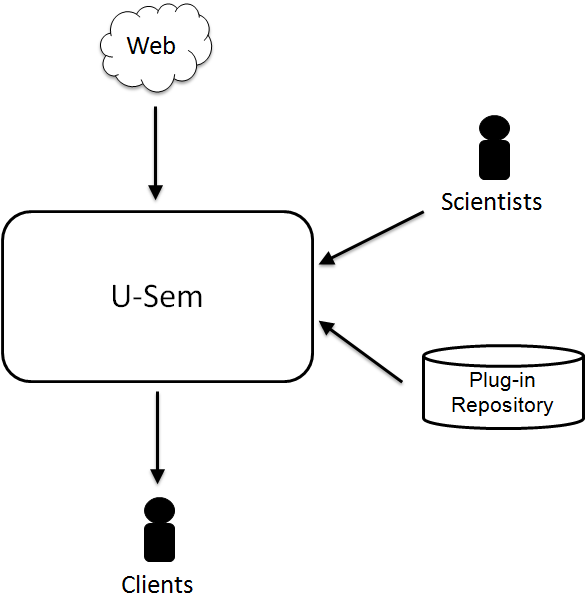
\includegraphics[scale=0.5]{plug-in/environment/runtime_env.png}
  \caption{Context diagram of U-Sem }
  \label{fig_context}
\end{figure}

\paragraph{Plug-in repository}
It represents a storage location where plug-ins are stored and when needed, they can be retrieved and installed into the system. Engineers build and then publish their plug-ins there so that anyone interested can install and use them. 


\subsection{Interactions}

After we have identified the new actors (engineers) and external systems(plug-in repository) in the environment of U-Sem we have to define how they interact with each other. In this section we use the Business Process Management Notation (BPMN) \cite{wohed2006suitability} to define the business processes that describe the interactions needed for each of the use cases regarding the dynamic component model feature of U-Sem. The notation enables us to model activities, decision responsibilities, control and data flows. The decision to use BPMN to define the interactions is based on its suitability for interaction modelling and the fact that it is more popular compared to its alternatives \cite{decker2008interaction}. Next subsections describe each of the defined processes and expand them into Business Process Diagrams (BPD).

\subsubsection{Create U-Sem Plug-in process}

\begin{figure}[h!]
  \centering
  	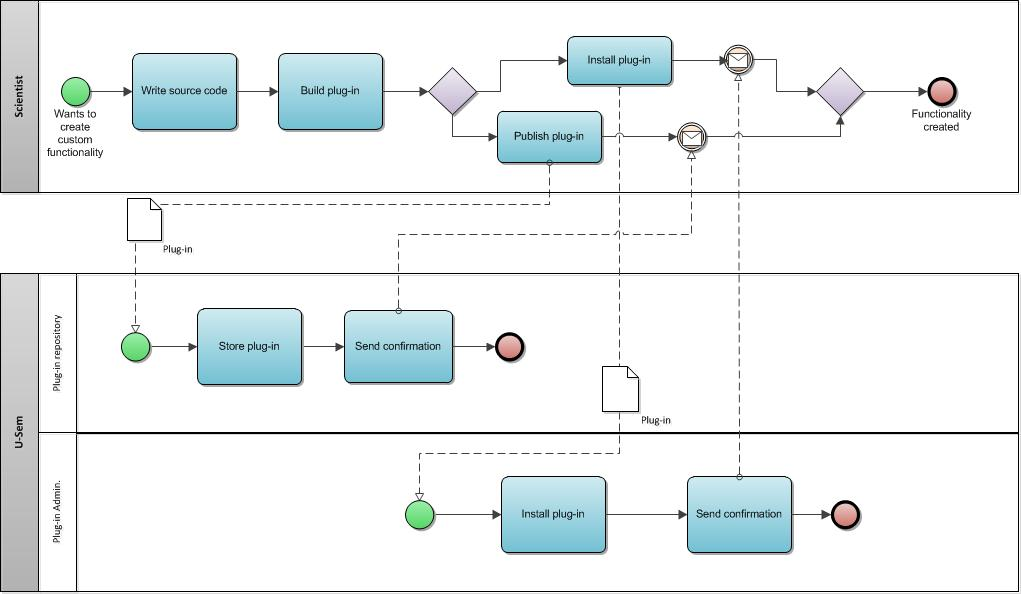
\includegraphics[scale=0.75,angle=270]{plug-in/business_processes/CreatePlugInBusinessModel.jpg}
  \caption{Business model describing the process for creating a new plug-in for U-Sem}
  \label{fig_install_bpm}
\end{figure}

In this section, we modelled the plug-in creation process as a business process. Figure \ref{fig_install_bpm} provides the business process model diagram that illustrates this process. 

As illustrated in the diagram, there are three participants in this process (U-Sem, Engineers and the Plug-in repository) which are illustrated in separate BPMN pools. When an engineer wants to create new functionality for U-Sem, he first writes the source code, providing all required resources and implementing the desired U-Sem interfaces (the component interfaces discussed in Section \ref{sec:pluginModulAndManag}). Then, everything is built and encapsulated into a single plug-in. If it is only for private use, engineers can directly upload it to U-Sem. When U-Sem receives a component it is responsible to install it into the engineer's dedicated storage space and make available all functionality provided by the component. Finally, U-Sem sends confirmation message back to the engineer. Alternatively, the engineer might also want to share the component with other engineers. In this case, the component is sent to the plug-in repository. When received, the repository is responsible to store it and make it available to the other engineers. Again, at the end a confirmation message is sent back to the engineer.

\subsubsection{Reuse shared plug-ins}

\begin{figure}[h!]
  \centering
  	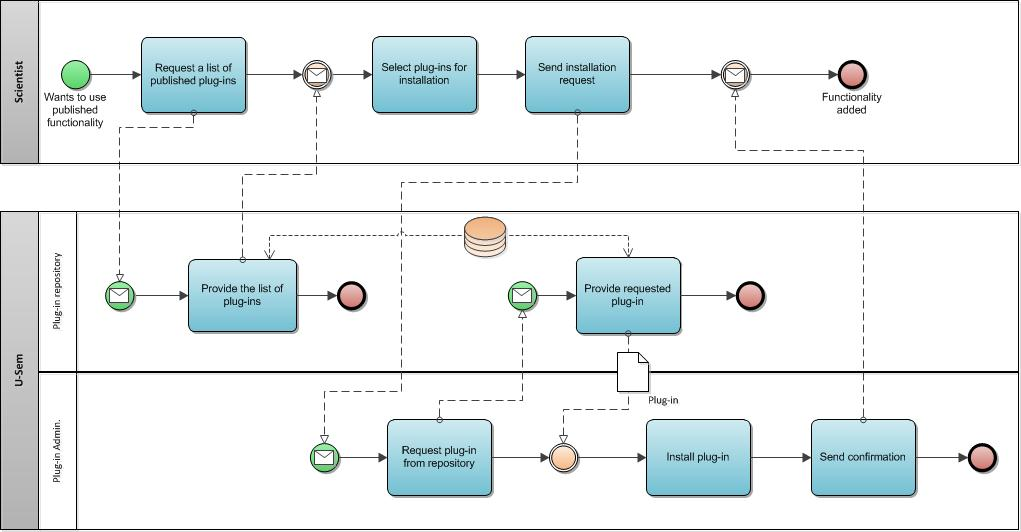
\includegraphics[scale=0.75,angle=270]{plug-in/business_processes/InstallPlugInFromRepoBusinessModel.jpg}
  \caption{Business model describing the process for installing a shared plug-in/s to U-Sem}
  \label{fig_repo_bpm}
\end{figure}

As defined in section \ref{sec:requirementsPlugin}, U-Sem also enables engineers to reuse plug-ins shared by others. This use case is also modelled as a separate business process which is illustrated in Figure \ref{fig_repo_bpm}. Again, we have three participants in this process (U-Sem, Engineers and the Plug-in repository) which are illustrated in separate BPMN pools. 

The process consists of two main phases. First, the engineer contacts the plug-in repository in order to determine what are the currently available plug-ins and then, he contacts U-Sem providing information about the desired plug-ins. Upon receiving the request, U-Sem is responsible to contact the plug-in repository and retrieve the requested plug-ins which are, at the end, installed into the private space of the engineer and a confirmation message is sent back.

\subsubsection{Plug-in Management}

\begin{figure}[h!]
  \centering
  	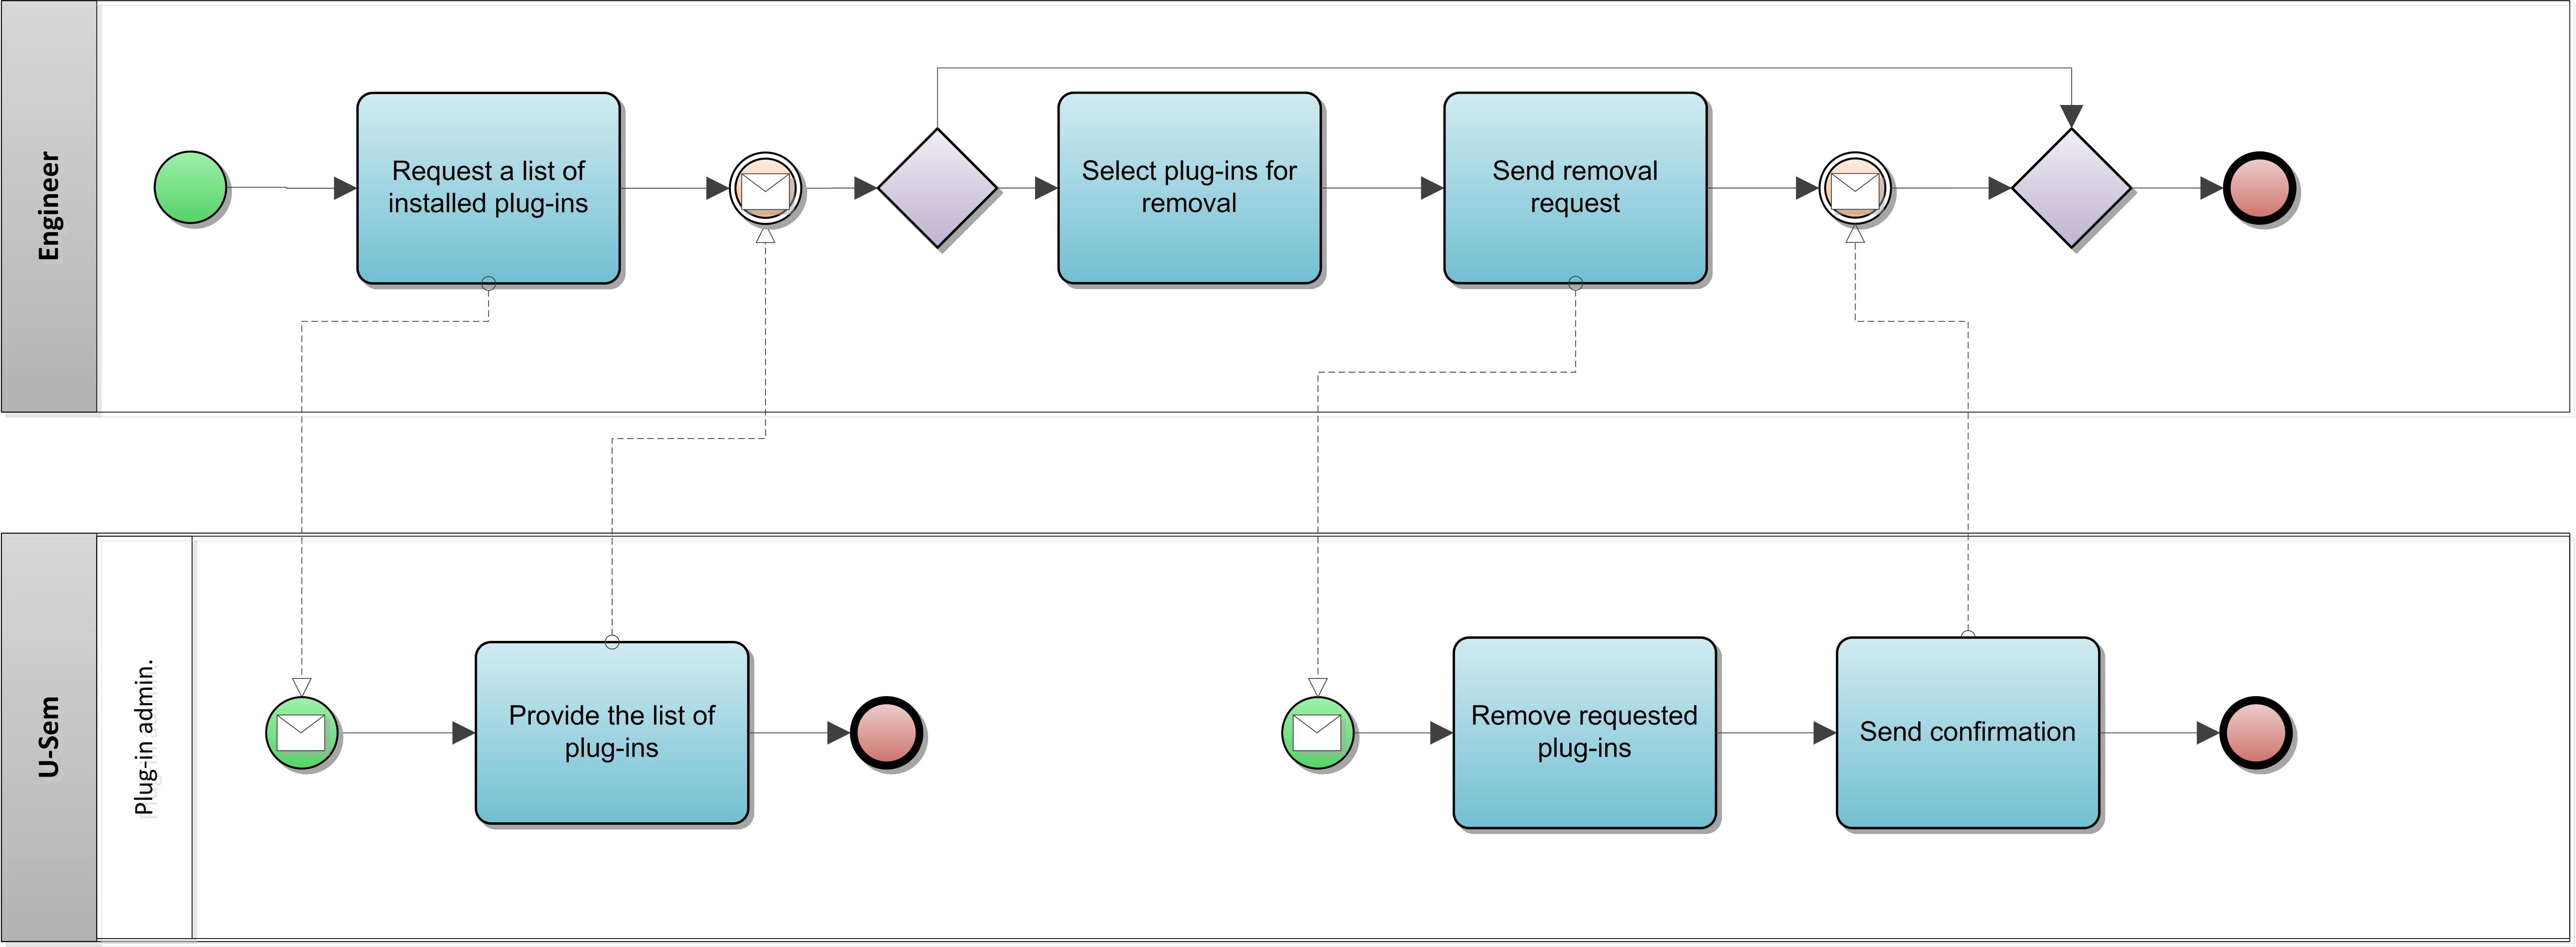
\includegraphics[scale=0.75,angle=270]{plug-in/business_processes/PluginManagementBusinessModel.jpg}
  \caption{Business model describing the process for managing plug-ins in U-Sem}
  \label{fig_admin_bpm}
\end{figure}

Managing plug-ins is also another important use case. Implementing it enables engineers to view all plug-ins installed into U-Sem and if needed remove any of them. This use case was modelled into the \textit{Plug-in Management process} which is illustrated on Fugure \ref{fig_admin_bpm}. In this case, we have interaction only between the engineer and U-Sem.

Engineers can monitor the currently installed plug-ins at any time by contacting U-Sem. When such request is received, U-Sem is responsible to send back detailed information about all the plug-ins. Having this list, engineers are also able to remove plug-ins. In this case, they have to submit request for removal providing details for the plug-in that has to be removed. Upon receiving a request for plug-in removal, U-Sem is responsible to permanently remove it form the private space of the engineer and when finished send back a confirmation message.


\subsection{Functional view}

After identifying all actors that are part of the environment of U-Sem and the way they interact with one another, in this section, we define the internal structure of U-Sem that is responsible to accommodate all these interactions. The functional structure of the system includes the key functional elements, their responsibilities, the interfaces they expose, and the interactions between them \cite{rozanski2011software}. All these together demonstrate how the system will perform the required functions.

All components that take part in the Plug-in Environment feature can be classified in three layers. This organization is illustrated in figure Figure \ref{fig_layer} and consists of the following layers:

\begin{figure}[h!]
  \centering
  	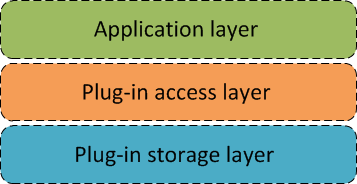
\includegraphics[scale=0.6]{plug-in/layers/layers.png}
  \caption{Layered organization of the solution}
  \label{fig_layer}
\end{figure}

\begin{itemize}
	\item \textit{Presentation layer} this layer consists of all functional components that are interested in using the services provided by the plug-ins and also the components that provide the user interface for adding new plug-ins to the system or managing the existing ones. 
	\item \textit{Plug-in access layer} provides functionality for plug-in management and also provides access to the services provided by the plug-ins. The functional components that build this layer are responsible to enforce the security and privacy policies of the system.
	\item \textit{Plug-in storage layer} is responsible to provide storage functionality for storing the installed plug-ins. Additionally, it should also provide place where plug-ins can store data during their execution.
	\end{itemize}

\subsubsection{High-level component organization}

This section describes the internal structure of the layers and identifies the high level components that build up the feature. Figure \ref{fig_funcorg} illustrates this organization. It shows how the high-level components are organized into the layers and the way they depend on each other. We have identified the following high level components:

\begin{figure}[h!]
  \centering
  	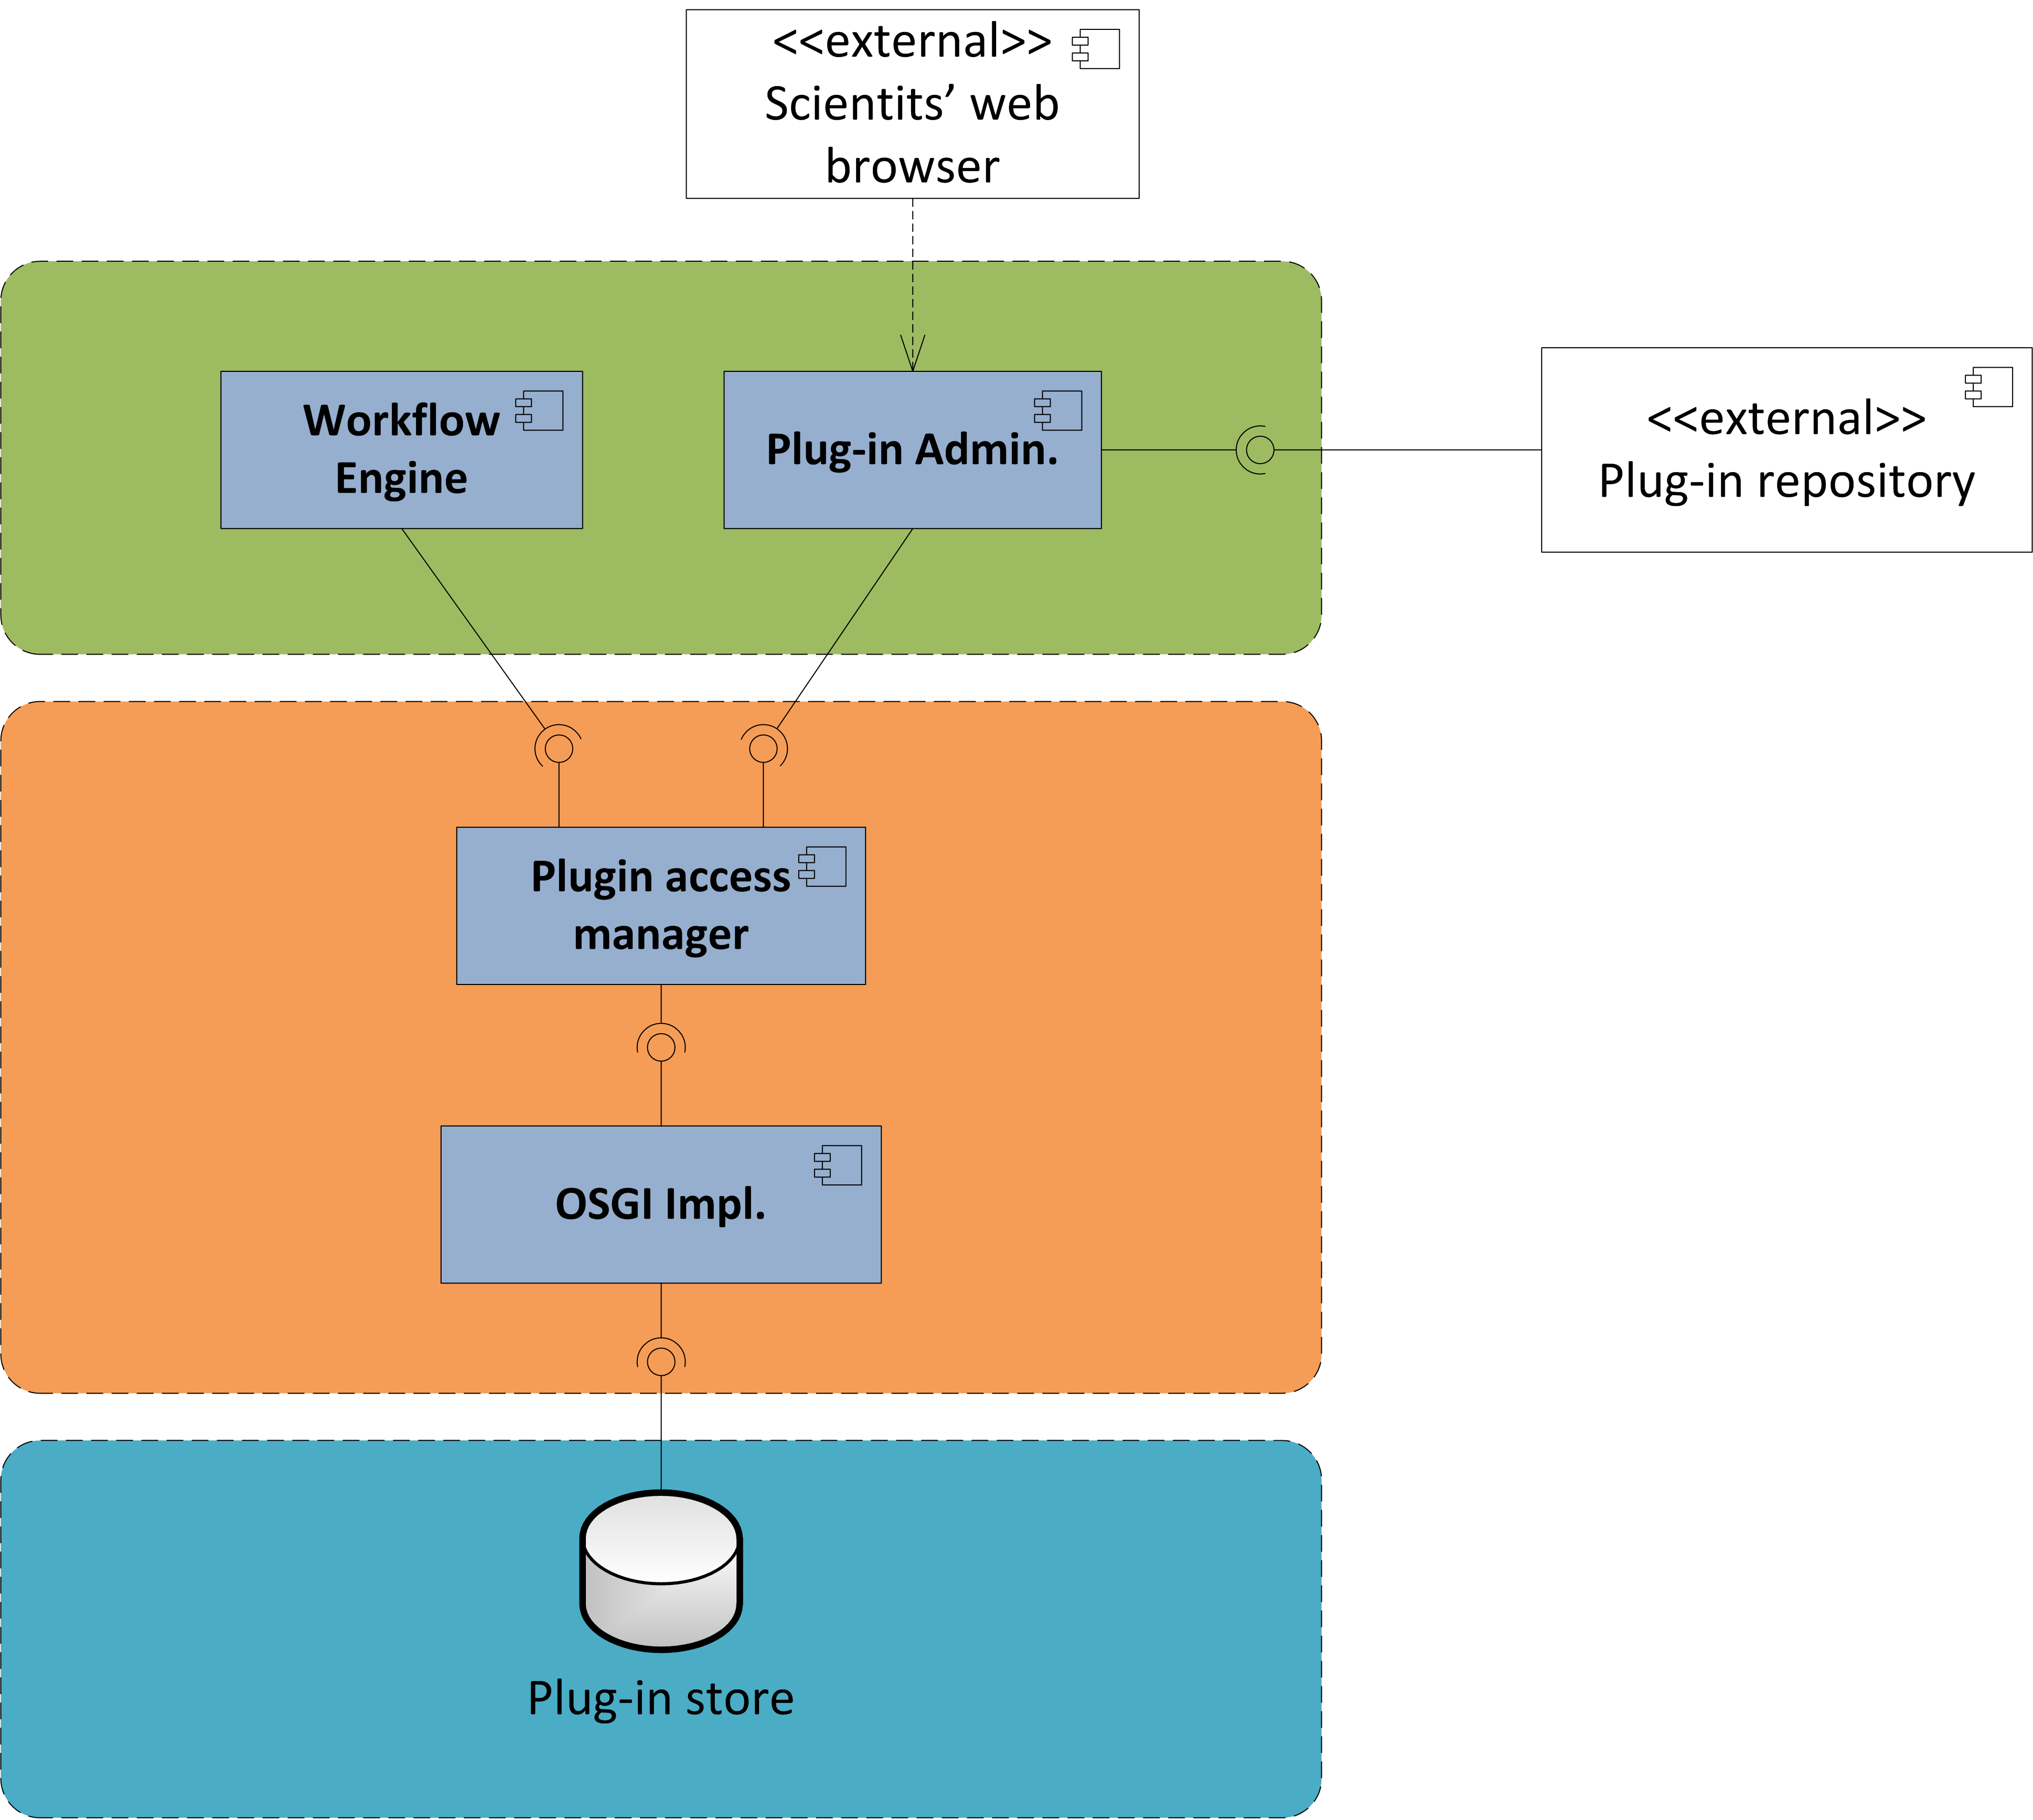
\includegraphics[scale=0.6]{plug-in/layers/main-func.png}
  \caption{Component diagram illustrating the functional organization of the solution}
  \label{fig_funcorg}
\end{figure}

\begin{itemize}

\item \textit{Plug-in Store} is responsible to store the installed plug-ins for each engineer. It should provide permanent store for the components so that after system restart they are still available. This component is also responsible to provide storage space for each component in case any data storage is required. The current state of the OSGi implementations only allows integration with file systems for plug-in storage and therefore, this component has to provide file system interface for communication.

\item \textit{OSGi Implementation} - As we already discussed in previous sections, we will use the OSGi standard as a base for providing the dynamic component model for U-Sem. It is responsible to mange the plug-ins' life cycle and provide access to the services provided by them. It provides an API which enables other components to communicate with the framework.

\item \textit{Plug-in access manager} acts as a level of abstraction over the OSGi component. It is responsible to deal with the configuration and manage the life cycle of the OSGi framework. It is also responsible to enforce the security policy and provide isolation between engineers. It provides API for the presentation layer components for accessing services and management of plug-ins. Further decomposition of this component is provided in the next sections.

\item \textit{Plug-in admin} is responsible to deal with the administration of the plug-ins. It provides the system's endpoints (user interfaces) for interaction with the engineers. Additionally, it also provides functionality for communication with the plug-in repository. Further decomposition of this component is provided in the next section. 

\item \textit{Workflow engine (RDF Gears)} uses the API provided by the \textit{Plug-in access manager} to access the services provided by the installed plug-ins. During the workflow configuration phase it obtains the list of available services, while during the workflow execution phase it uses the API to execute and retrieve the result of the services.
	
\end{itemize}


\subsubsection{Plug-in admin}

This section defines the functional decomposition of the \textit{Plug-in admin} component which is illustrated on Figure \ref{fig_admin_func}. It consists of the following components:

\begin{figure}[h!]
  \centering
  	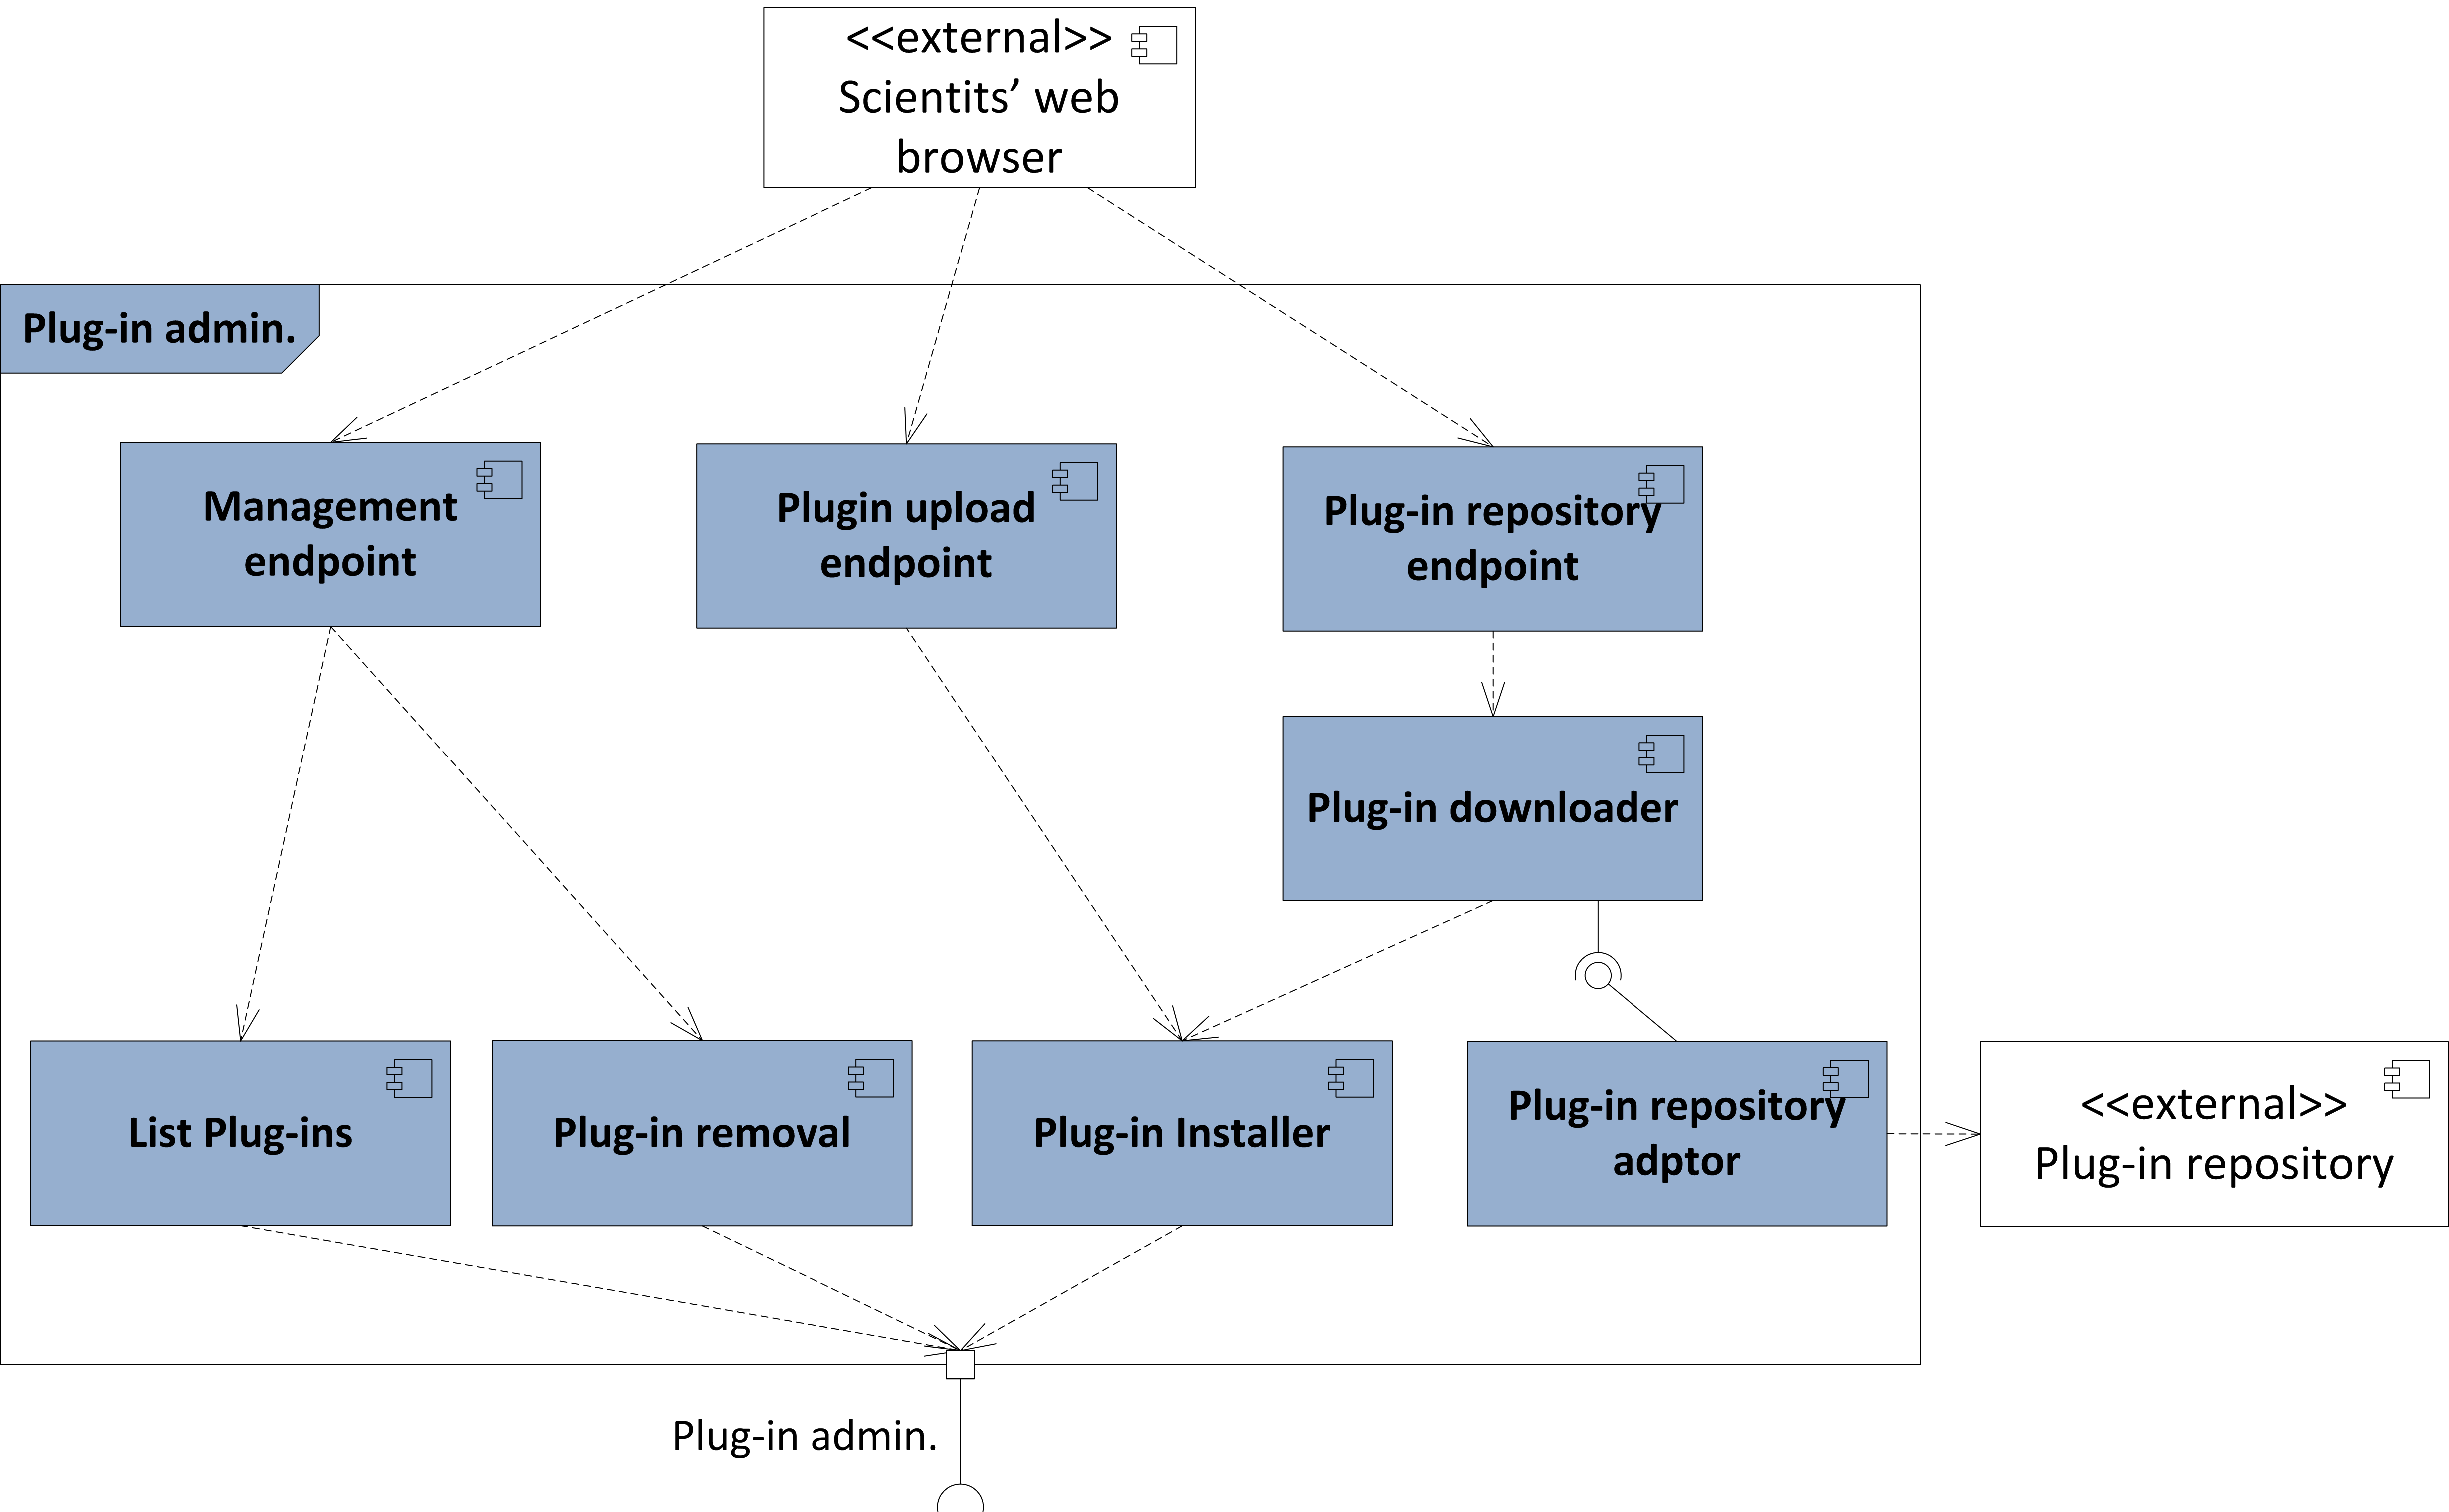
\includegraphics[scale=0.75]{plug-in/layers/admin-func.png}
  \caption{Functional decomposition of the \textit{Plug-in admin.} module}
  \label{fig_admin_func}
\end{figure}

\begin{itemize}

\item \textit{Management endpoint} - This component provides the user interface for the plug-in management. It acts as a bridge between the engineer and the Plug-in admin API provided by the \textit{Plug-in access manager}. It uses the API in order to present the current state of the system to the engineers and also enable them to remove any components. This component also checks the dependencies between the installed plug-ins and notifies the engineer if any of them are missing.

\item \textit{Plug-in upload endpoint} - This components provides the user interface needed for uploading plug-ins. It enables engineers to select a \textit{jar} file from their local file system and upload it for installation. When the plug-in is uploaded to U-Sem it is installed using the Plug-in admin API.

\item \textit{Plug-in repository endpoint} - This component provides the user interface which enables engineers to browse the plug-in repository and indicate which plug-ins should be downloaded and installed on U-Sem. It checks the dependencies of the selected plug-ins and if any are missing it notifies the engineer and proposes to install the missing plug-ins as well. Finally, the selected plug-ins are downloaded from the repository and upon successful download they are installed using the Plug-in admin API.

\item \textit{Plug-in repository adaptor} - This component manages  the communication with the plug-in repository. It acts as a level of abstraction over it. U-Sem might evolve in future and need to use different repositories and in that case, this is the only component to change if support for a new repository system is needed. 

\end{itemize}


\subsubsection{Plug-in access manager}

This component is responsible to provide API which can be used by presentation layer components in order to manage the plug-ins and access the services provided by them. Figure \ref{fig_access_func} shows the functional decomposition of the Plug-in access manager module. It consists of the following components:


\begin{figure}[h!]
  \centering
  	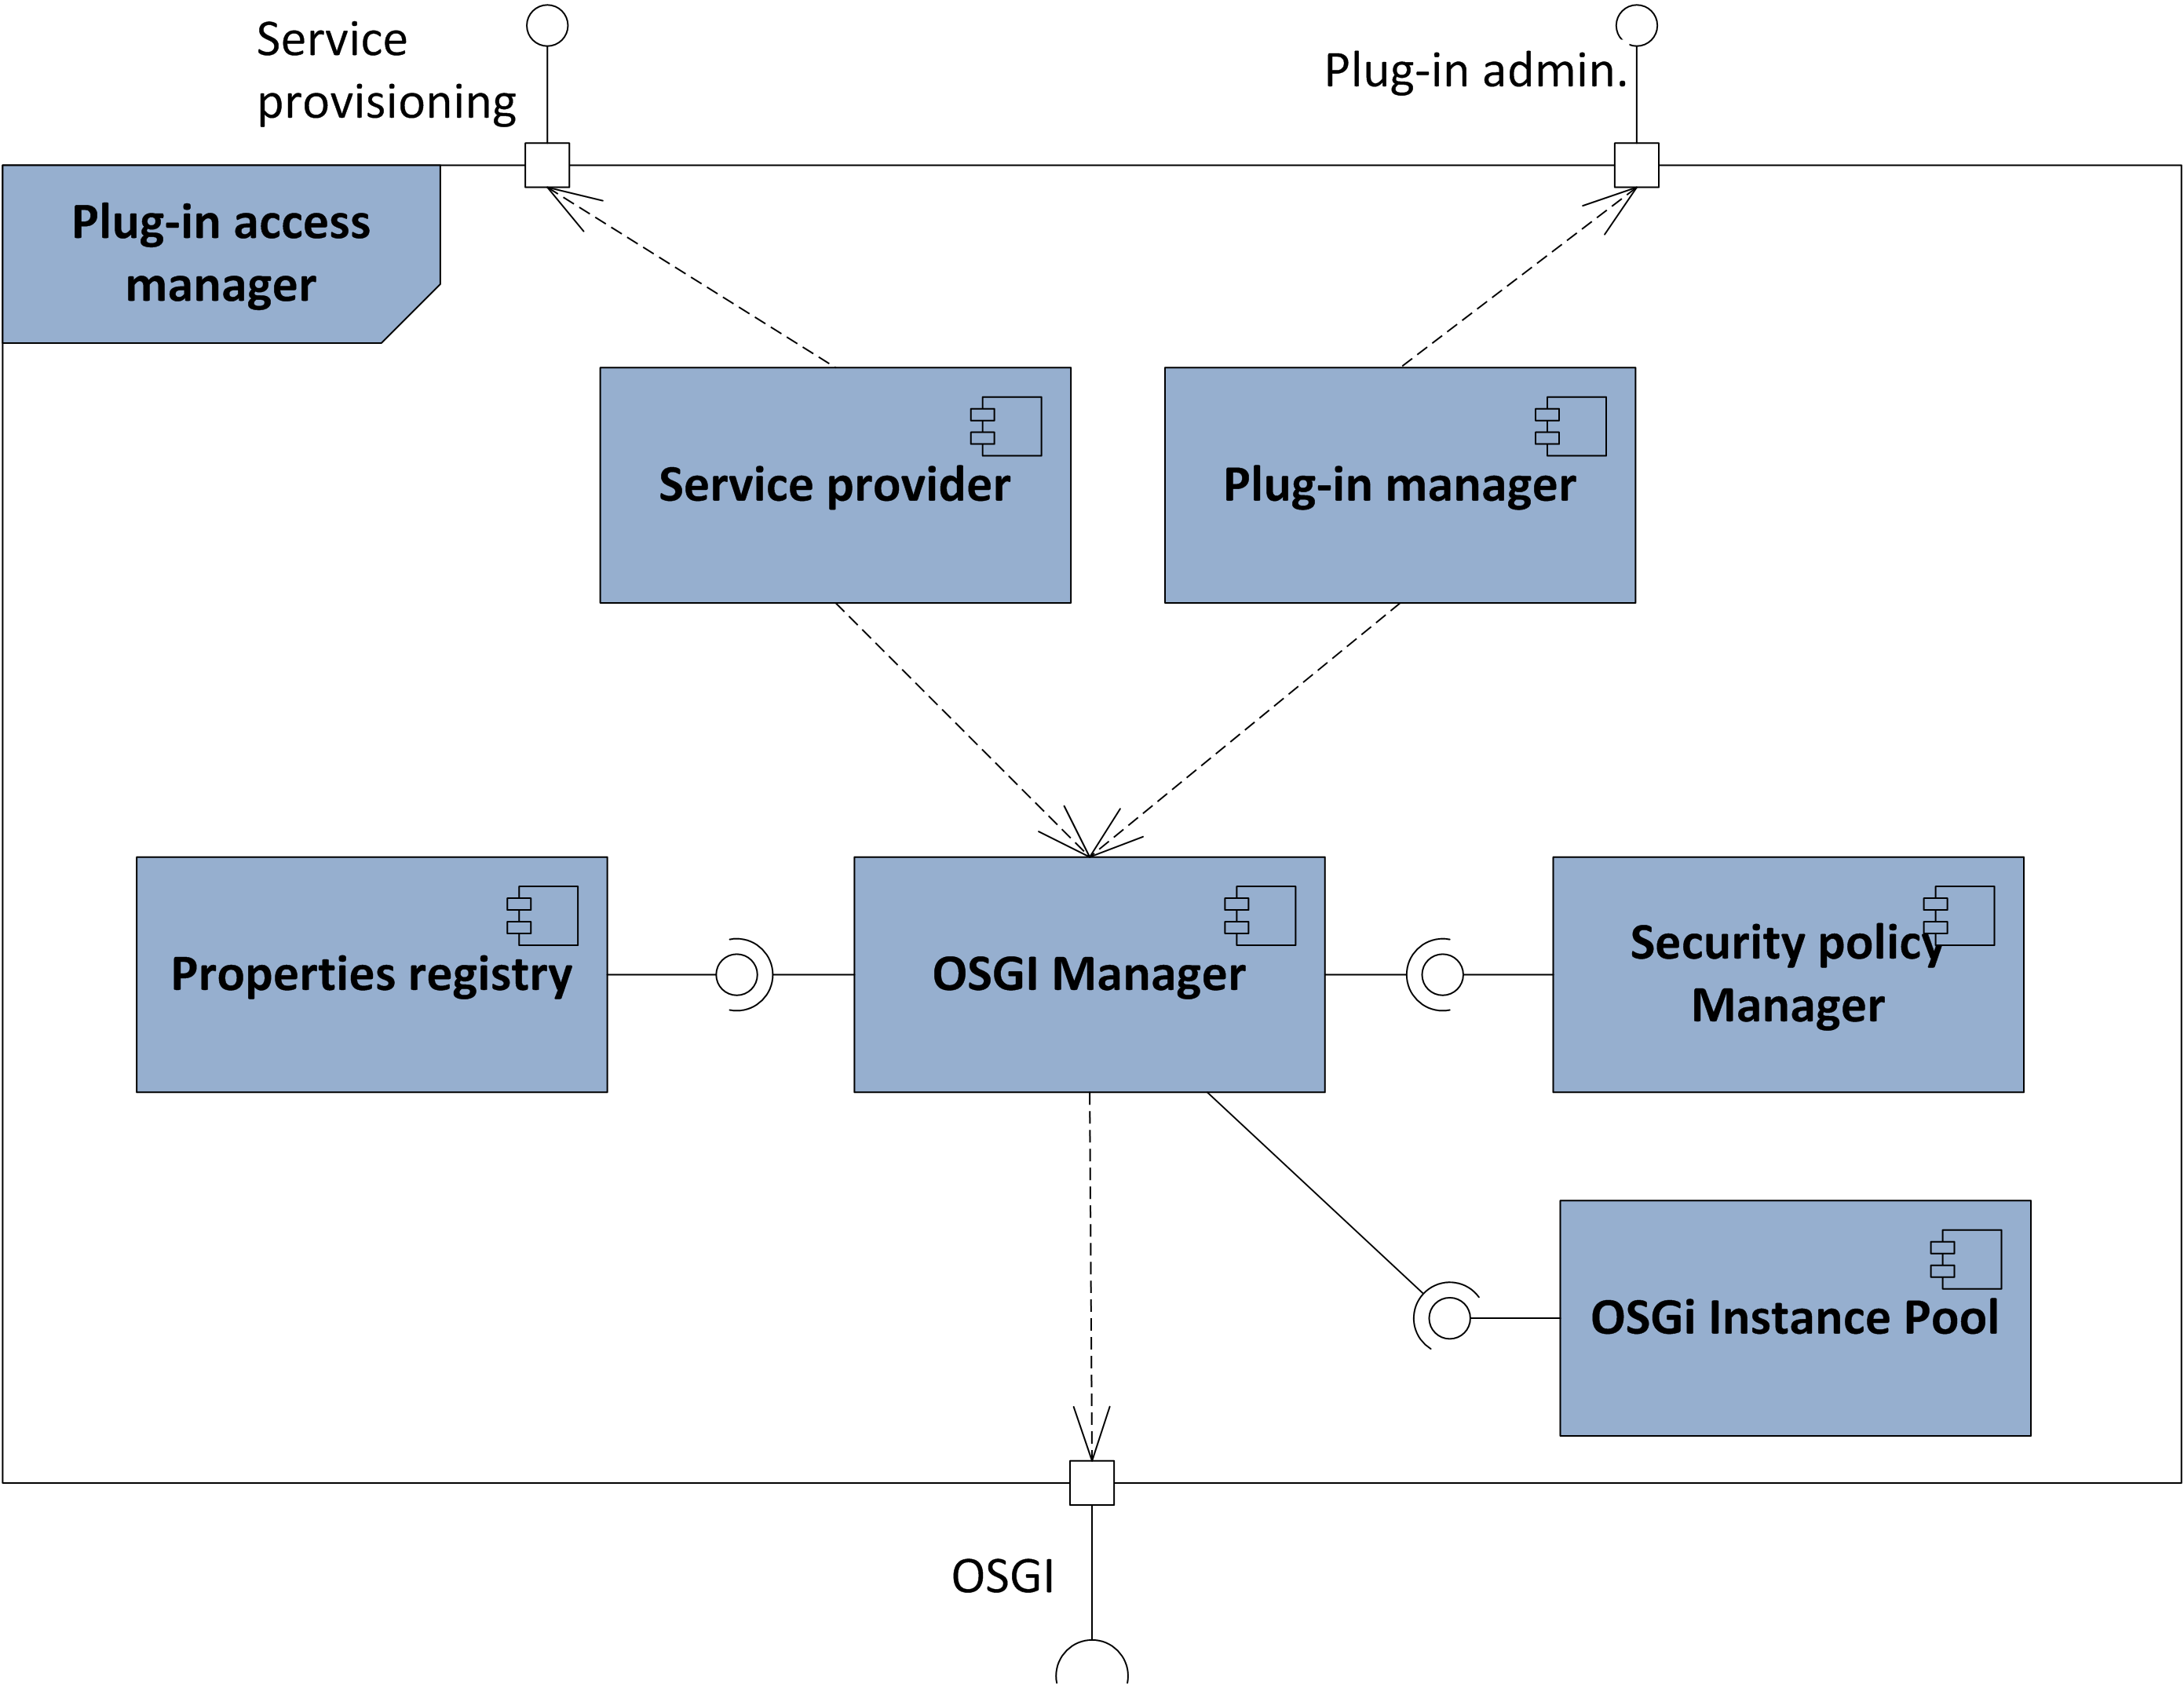
\includegraphics[scale=0.85]{plug-in/layers/access-func.png}
  \caption{Functional decomposition of the \textit{Plug-in access manager} component}
  \label{fig_access_func}
\end{figure}

\begin{itemize}

\item \textit{OSGi Manager} - This component manages the communication with the OSGi framework. It is responsible to start/stop the framework and monitor its life cycle. All needed properties for the framework operation are provided by the \textit{Properties registry} component. The OSGi Manager is also responsible to enforce the security policies by setting up the Security Manager options provided by the \textit{Security policy} component. It also acts as a level of abstraction over the plug-in engine and in case any change in future is required, this is the only component that will be affected. 

Starting an OSGi instance can be a time costly procedure especially when there are a lot of plug-ins to be loaded. Therefore, in order to increase the performance of the system with the help of the \textit{OSGi Instance pool} component when an OSGi instance is no longer needed it is not destroyed but cached so that it can be later reused and not created again.

\item \textit{OSGi Instance pool} - based on the connection pool idea \cite{zhao2004design}, this component provides a cache for OSGi instances so that they can be reused when future interactions with the plug-ins are required.

\item \textit{Properties registry} - Keeps track of all common and user related options that are required for the correct operation of the OSGi framework. The main properties this component is responsible to provide are the paths to the plug-in storage space for each engineer. It has to make sure that this spaces are not overlapping. Additionally, it also provides information about the security policy that has to be applied to a particular engineer. 

\item \textit{Security policy manager} - This component is responsible to provide access to the security policies of U-Sem which define the operations that the custom code loaded by the framework is allowed to perform.

\item \textit{Plug-in manager} - This component is responsible to provide an API for the \textit{Presentation layer} components that enables them to perform plug-in management tasks.

\item \textit{Service provider} - This component is responsible to provide an API for the \textit{Presentation layer} components that enables them to access the services implemented by the loaded components in U-Sem.

\end{itemize}

\subsection{Concurrency view}
\label{sec:pluginConcur}

This section describes the concurrency structure of U-Sem. We show how functional elements map to concurrency units (processes, process groups and threads) in order to clearly identify the parts of the system that can work concurrently. We also show how this parallel execution is coordinated and controlled.

\begin{figure}[h!]
  \centering
  	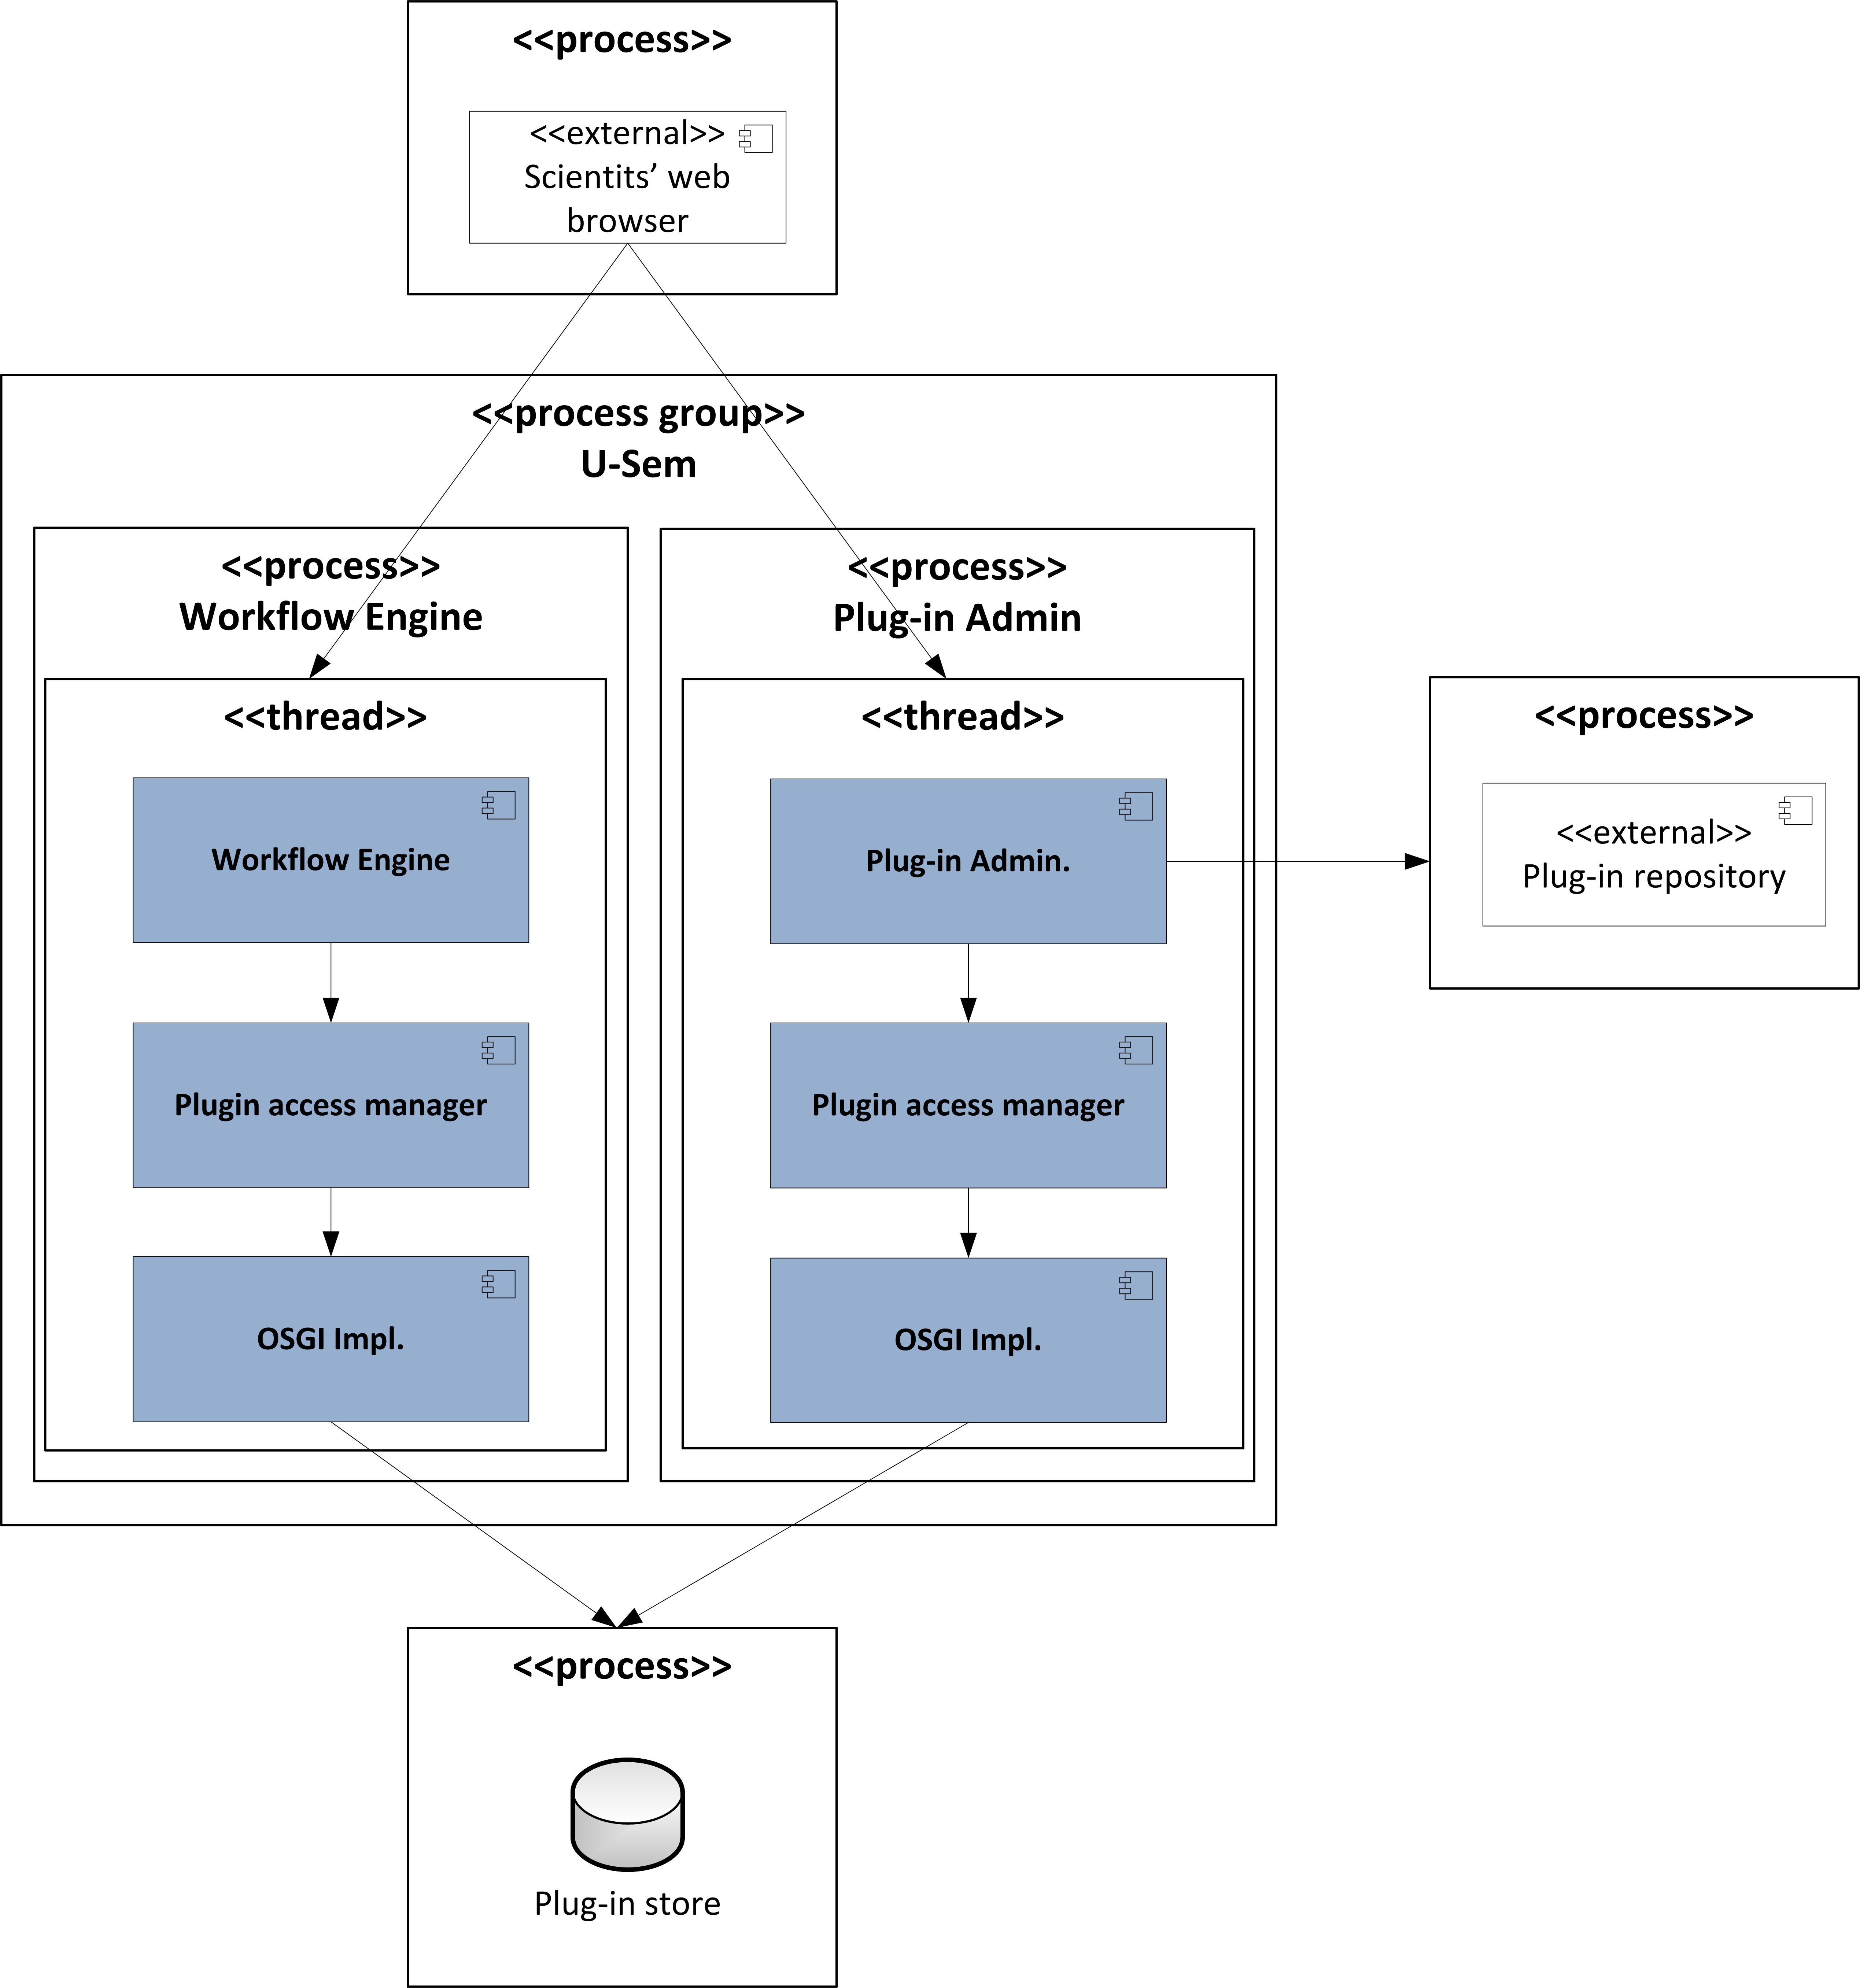
\includegraphics[scale=0.70]{plug-in/layers/concur.png}
  \caption{Diagram illustrating the concurrency model of the solution}
  \label{fig_conc}
\end{figure}

Figure \ref{fig_conc} illustrates the concurrency organization of U-Sem. The main functionality of the system is situated in the U-Sem process group. All U-Sem processes and all external processes (Plug-in repository) including the Plug-in store process operate concurrently. The main processes wait for requests from the user (web browsers and/or other systems). Each request is processed in a separate thread depending on its type (workflow or plug-in management). As a result, multiple client requests can be handled simultaneously. The main idea behind this design is to separate the workflow and the Plug-in administration functionality into separate processes which enhances loose coupling and, hence, improves maintainability and simplifies upgrades to new versions of the workflow engine. Additionally, if in future there is a need for higher performance the workflow engine process can be replicated without affecting the plug-in administration functionality. This organization, however, also introduces some problems that have to be solved.

\subsubsection{Problems}

The first problem lies in the fact that plug-in installation (plug-in admin.) and loading of plug-ins (workflow engine) are two actions that are completely independent from each other. Therefore, if the wokrflow engine tries to load the plug-ins when the plug-in admin. is in the middle of installation then they may fail to load or load incorrectly. 

Secondly, as discussed in the previous section the system maintains a pool with the OSGi instances so that they can be reused instead of loaded from scratch. However, whenever a plug-in is installed or removed these cached instances become obsolete and have to be discarded. In order to do that, the plug-in admin. has to notify the workflow engine for the change in the plug-ins which is a problem when the two components are in separate processes.

\subsubsection{Solution}

In order to solve the first problem we propose a solution that is based on synchronization between the processes. It is based on the \textit{Reader-Writer Lock} idea which enables concurrent read access to a shared resource but requires exclusive access for write operations \cite{lev2009scalable}.

Our solution maps to the \textit{Reader-Writer Lock} idea as follows:
\begin{itemize}
	\item The shared resource is the plug-in store allocated to an engineer.
	\item The workflow engine acts as reader of the shared resource.
	\item The plug-in administration acts as writer of the shared resource.
\end{itemize}

As a result, when a change to the plug-ins is needed it is executed exclusively and any components that want to load the plug-ins have to wait until the change is applied. Therefore, the workflow engine is protected against loading the plug-ins while they are inconsistent. This approach has the benefit that loading plug-ins is not exclusive and can be done simultaneously by many components and therefore, the concurrent configurations and executions of workflows are not affected. 

The standard \textit{Reader-Writer Lock} in Java, however, works only within the virtual machine\footnote{Java Documentation - http://docs.oracle.com/}. In our case we have to synchronize entire processes. Our research showed that there are already existing tools that provide this functionality \cite{hernane2012dynamic} and therefore, we decided to reuse one of them. The tool that is used in the proposed solution is Terracotta\footnote{Terracotta - http://terracotta.org/}. It introduces a process that is responsible to provide the lock and the other processes communicate with it in order to obtain it and use the resources.

In order to solve the second problem we extend the architecture by providing mechanism for inter-process communication in order to enable the plug-in admin to notify all processes for any updates so that they can clean their caches. The general idea is that all components that maintain caches register to receive updates when plug-ins change. Whenever a change occurs all registered components are notified using a broadcast protocol \cite{joseph1988reliable}. Our research showed that the Terracotta system that we use to solve the first problem also provides implementation of a broadcast protocol. Therefore, when a workflow engine loads the plug-ins it contacts the Terracotta process and registers itself for updates regarding the plug-ins. When an engineer removes or installs a plug-in the plug-in admin contacts the Terracotta process which then notifies all the registered processes.\\

Having presented the most important features of the architecture of the solution we continue by discussing its implementation in next section. 


\section{Implementation}
\label{sec:implPlugin}

We implemented the proposed architecture in order to evaluate its applicability and capabilities. This section describes the main steps we performed during the implementation of the system.

First, we had to choose which OSGi implementation to use. Nowadays there are several vendors that provide implementations. The most popular are: Equinox\footnote{Equinox - http://www.eclipse.org/equinox}, Felix\footnote{Apache felix - http://felix.apache.org} and Knopflerfish\footnote{Knopflerfish - http://www.knopflerfish.org} \cite{tavares2008gentle}. Theoretically, they all strictly implement the OSGi standard and therefore, there should be little difference. However, we choose Equinox because it seems more matured and more widely used compared to the others. Moreover, Equinox is highly integrated in the popular Eclipse IDE. This enables engineers to use the out-of-the box functionality for creating plug-ins in Eclipse.

Secondly, we had to identify the kind of OSGi services that can be provided by plug-ins so that we can define the required interfaces. Looking at the requirements, we identified that engineers have to be able to provide custom workflow functions and entire workflow definitions. As described in Section \ref{sec:pluginModulAndManag}, in OSGi services are defined as Java interfaces or classes. For providing custom workflow functions engineers can directly reuse the \textit{RGLFunction} class which is part of RDF Gears. The situation with the workflows, however, is more complicated since they are represented as resource (XML) files. OSGi does not provide direct way for providing resource files as services. In order to overcome this problem, we defined a new class called \textit{WorkflowTemplate} which acts as a bridge and enables the workflow engine and other components to access workfow definition files provided by plug-ins.

\begin{figure}[h!]
  \centering
  	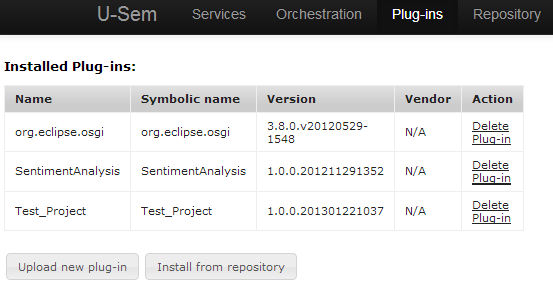
\includegraphics[scale=0.70]{plug-in/ui/list.png}
  \caption{User interface for plug-in management.}
  \label{list_ui}
\end{figure}

Next, we provided an experimental implementation of the plug-in repository. It represents a simple web application which stores the plug-ins locally into the file system of the web server where it is deployed. The implementation provides REST interfaces for retrieving the list of available plug-ins and providing the contents of a selected plug-in. It also includes user interface which enables engineers to upload their plug-ins. 


\begin{figure}[h!]
  \centering
  	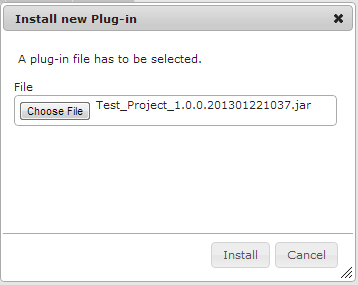
\includegraphics[scale=0.6]{plug-in/ui/upload.png}
  \caption{User interface for uploading and installing plug-ins in U-Sem.}
  \label{upload_ui}
\end{figure}

We continued by implementing all the components defined in the proposed architecture of U-Sem. In order to implement the endpoints we used the jQuery UI\footnote{jQuery - http://jqueryui.com/} and Bootstrap\footnote{Bootstrap - http://twitter.github.com/bootstrap/} user interface technologies. Figure \ref{list_ui} presents the endpoint for viewing all installed plug-ins. The detailed information about all installed plug-ins is represented in a table. Each row has a "Delete" button which provides access to the functionality for removing plug-ins. At the bottom of the view, there are two buttons that lead to the endpoints for uploading a plug-in depicted in Figure \ref{upload_ui} and the endpoint for browsing and installing plug-ins from the repository depicted in Figure \ref{repo_ui}.

\begin{figure}[h!]
  \centering
  	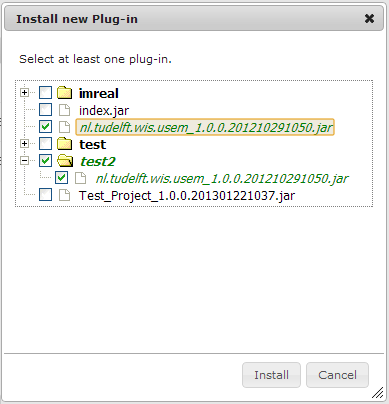
\includegraphics[scale=0.6]{plug-in/ui/repo.png}
  \caption{User interface for browsing and installing plug-ins from the plug-in repository.}
  \label{repo_ui}
\end{figure}

Finally, we simplified the deployment of the solution by constructing a build script that packs all source files into deployable components (war files) that can be directly deployed to a web server. Furthermore, we also prepared a tutorial presented in Appendix \ref{cha:tutorial} which aims to help engineers quickly learn how to work with the new solution.

\section{Evaluation}
\label{sec:evalPlugin}

After successfully implementing the system, in this section we evaluate whether the system actually solves the problems identified in Section \ref{sec:problemDefPlugin}. In order to do the evaluation we asked engineers to use the new solution to implement real-world user modelling services and asked them to comment on the problems the solution is designed to solve. The following is summary of the engineers feedback:

\begin{itemize}
	\item The introduced solution saves time and efforts to the engineers. This is because the task of adding functional components to U-Sem is significantly simplified. Engineers no longer have to modify, build and deploy the entire workflow engine every time they perform the task. Instead they can develop their functional components separately from the wokflow engine and install them when needed. This activities are also automated and require almost no overhead work from the engineers. 
	
	\item Engineers reported that the time needed for training new engineers to work with the system is significantly reduced. Because of the simplified process they do not have to learn how to check out, modify, build and deploy the workflow engine. Instead they only have to learn how to build the plug-ins and install them to the system which is facilitated by the specially prepared tutorial.
	
	\item Engineers no longer disrupt each others work because adding functional components to the system is performed in isolation for each of them and there is also no need for restarting the system. 
	
	\item The versioning issue explained in Section \ref{sec:problemDefPlugin} is no longer a problem because engineers deploy and use the plug-ins in isolation between each other and there is no way that one engineer can modify the plug-ins of another.
	
	\item Engineers also reported that the implementations of the functional components are no longer so tightly coupled between each other because the source code is no longer freely available as part of the workflow engine. It is now owned by the engineers themselves and using the information hiding mechanisms of OSGi they can define more precisely which part of their code can be accessed and which not.
	 
\end{itemize} 

Analysing this feedback we can conclude that we have solved the problems defining the Plug-in Environment feature and the designed and implemented system is capable of serving its intended purpose. As in most scientific works, however, there is still some place for improvement in this one as well. In next section we discuss possible directions for future work regarding the feature.


\section{Limitations and Future Work}
\label{sec:limitsPlugin}

In this section we identify the limitations of the proposed architecture and we also suggest approaches that can be used to overcome some of these limitations in future. We have identified two groups of limitations. The first group represents the limitations that are inherited from the usage of OSGi. The second one consists of the limitations concerning the rest of the architecture.

Most of the limitations concerning OSGi originate from the potential vulnerabilities of running external code which the security mechanism fails to fully address. The authors of \cite{parrend2009security} have studied in details the potential vulnerabilities of OSGi. These vulnerabilities can be grouped into the following categories:

\begin{itemize}

	\item \textit{Vulnerabilities on operating system level} - This kind of vulnerabilities result from the fact that it is possible that a plug-in runs malicious native code using the Java JNI. Native code is not managed by the JVM and thus, the security policy is not applied. \cite{sun2012jvm} proposes a portable solution for sandboxing of Java's Native Libraries without modifying the JVM's internals which might be used for overcoming these vulnerabilities.
	
	\item \textit{Vulnarabilities on OSGi platform level} - This kind of vulnerabilities are related to weaknesses in the OSGi run-time. \cite{parrend2009security} suggests an approach for overcoming them by adding additional security checks in the OSGi implementation.
	
	\item \textit{Vulnarabilities on JVM level} - This vulnerabilities can be further divided into categories \cite{geoffray2009jvm}: 
	
	\begin{itemize}
		\item \textit{lack of isolation} - Even though components for each user are loaded through separate OSGi instances, on JVM level \textit{java.lang.Class} objects and static variables are shared by all plug-ins. A malicious bundle can interfere with the execution of other bundles by altering static variables or obtaining lock on shared objects.
		
		\item \textit{lack of resource accounting} - In OSGi each plug-in is loaded with a separate class loader. However, JVM does not perform resource monitoring on a per class loader basis. Therefore, in case of the overuse of resources (CPU, memory), it is impossible to identify the faulty bundle and stop its execution.
		
	\end{itemize}
	
	\cite{geoffray2009jvm} proposed and approach for overcoming these vulnerabilities. They have designed I-JVM, an extension of the Java Virtual Machine which provides functionality for component isolation and termination in OSGi.
	
\end{itemize}

At this point, U-Sem is aimed to be used by engineers from a single organization. Therefore, the components will only be reused within the organization which limits the possibility for any external person adding plug-ins into the system. Therefore, exploitation of the discussed vulnerabilities on purpose is not so likely. Therefore, we believe that this limitations does not pose a significant threat for U-Sem. However, all these vulnerabilities have to be addressed if in future the system is to be extended to give access to unverified engineers. 

The second group of limitations and possible future work concerns mainly the collaboration mechanism. In this work we provide a simple implementation of a Plug-in Repository which main purpose is to prove our concept. Introducing more sophisticated repository implementation which provides access and version control mechanisms for the plug-ins might be beneficial for the engineers in future. Finally, extending the plug-in dependency management capabilities of the solution so that it is capable to detect "indirect" dependencies between plug-ins is considered as another interesting topic for future research.

\chapter{Data Management} 
\label{cha:data}

This chapter proposes a solution to the \textit{Data Management} problem in U-Sem. Section \ref{sec:storageReq} identifies all functional and non-functional requirements that a successful solution must satisfy based on the problems discussed in Section \ref{sec:problemDefStorage}. Section \ref{sec:approachStorage} discusses that state of the art approaches and technologies that  can contribute to solving the problem. Section \ref{sec:architectureStorage} describes the software architecture that we propose in order to solve the problem. In Section \ref{sec:implStorage} we discuss the implementation that we provide in order to be able to verify the capabilities of the proposed architecture. Section \ref{sec:evalStorage} evaluates whether the proposed solution solves all of the defined problems. Finally, in section \ref{sec:limitsStorage} we discuss the limitations of the proposed design and suggest aspects in which the solution can be improved in the future.

\section{Requirements}
\label{sec:storageReq}

Having all concerns discussed in Section \ref{sec:problemDefStorage} in mind, we devised a complete set of requirements that present the functional scenarios (functional requirements) and system qualities (non-functional requirements) that the proposed architecture has to provide.

\subsection{Functional Scenarios}
In this section we formally identify the functional requirements which define the main interactions between the engineers and the system. Each scenario is marked with a code at the beginning which is used for easier identification during the verification and evaluation phase.

\begin{itemize}

	\item \textbf{UC1 - Insert data} - The system has to provide RDF Gears component and also API that can be used to store data.

	\item \textbf{UC2 - Update data } - The system has to provide RDF Gears component and also API that can be used to update existing data or part of it.
	
	\item \textbf{UC3 - Delete data} - The system has to provide RDF Gears component and also API that can be used to delete existing data or part of it.
	
	\item \textbf{UC4 - Query data} - The system has to provide RDF Gears component and also API that can be used to query existing data.
	
	\item \textbf{UC5 - Collaboration} - The system has to enable engineers to collaborate on data level by accessing and manipulating each others data. The system has to enable engineers to manage the privacy of their data. They have to be able to define whether their data (or parts of it) can be accessed and manipulated by the other engineers.

\end{itemize}

\subsection{Non-functional requirements}
This section identifies the main quality scenarios that a successful architecture has to accommodate.

\begin{itemize}
	\item \textit{Privacy} - the solution has to ensure the privacy of the stored data. The only way of interaction between engineers has to be achieved through the collaboration mechanism.
	
	\item \textit{Compliance} - the solution has to ensure that the newly introduced RDF Gears components comply with the RDF Gears specification. 
	
	\item \textit{Configuration management} - in order to simplify the configuration procedure of the system it should enable engineers to provide all the required configuration information concerning the new types of components within the plug-ins that define them. In this way, apart from the plug-in installation no additional work is needed in order to use the components.
	
\end{itemize}

\section{Approach}
\label{sec:approachStorage}

In this chapter we device a framework that is responsible to provide the Data management functionality for U-Sem. By carefully analysing the requirements defined in Section \ref{sec:storageReq} we concluded that the problem can be broken down into the following sub-problems:
\begin{itemize}
	\item \textit{Data storage and retrieval} - enable RGL oriented workflow engines (in our case RDF Gears) to hold their long-term data safely in a database and access it when needed.
	\item \textit{Multi-engineer support} - enable multiple engineers to work simultaneously with the solution and enable them to collaborate together in a controlled and secure fashion.
	\item \textit{RDF Gears extension} - ensure and if required extend the workflow engine so that it is able to deal with this new type of components correctly and efficiently.
	\item \textit{Integration with the Plug-in Environment feature} in order to simplify plug-in installation and configuration.
\end{itemize}

Next subsections explain how each of the sub-problems is approached and solved.

\subsection{Data storage and retrieval}

The main objective of this chapter is to facilitate the data storage process in U-Sem so that engineers can store and retrieve their data without having to bother how and where it is actually stored. Therefore, in order to achieve that we introduce a simplified abstraction layer which hides the actual storage implementation. Engineers only interact with the abstraction layer and they are not concerned about any implementation details. In the next subsection we discus the proposed abstraction which is followed by presentation of the approach we propose in order to implement it.

\subsubsection{Abstraction}

In order, to simplify the work of engineers we introduce an abstraction layer which requires engineers to only configure a set of predefined components in order to work with the data. This components are implemented as RDF Gears components and can be configured only by using the user interface. We introduce the following components which enable engineers to perform data operations:

\begin{itemize}
	\item \textit{Store} - this component is responsible to store its input data into the database.
	\item \textit{Update} - this component is responsible to replace existing data or parts of it with the provided input data.
	\item \textit{Delete} - this component is responsible to remove data identified by the engineer.
	\item \textit{Query} - this component expects a query as input and is responsible to execute it and provide the results as an output for the component.
\end{itemize}

There are two issues that have to be further discussed regarding these components. The first one concerns how the stored data is organized and the second one concerns the query mechanism.

\paragraph{Structure and Semantics of the data}
Section \ref{sec:problemDefStorage} makes clear that engineers' needs regarding data storage vary greatly and may also change in time. It is hard to predict and define the structure and semantics of all data that engineers might like to store. Therefore, a more generic solution is needed. The solution enables engineers to define the semantics and structure of the data they want to store on demand. This structure can be adapted over time if/when engineers' needs change. In this work we refer to each data entry as \textit{entity}, each group of entities that have the same semantics and structure as \textit{entity types} and the information that defines the structure and semantics of each entity type as \textit{entity definition}. All data in RDF Gears is presented in the RGL format and therefore, the intuitive approach is to provide engineers functionality that enables them to define these entity types in terms of RGL values. 

\paragraph{Querying data}

As specified above providing queries is needed in order to configure some of the components. The abstraction has to provide querying language that enables engineers to define queries in terms of the predefined entity definitions. There are two types of queries:

\begin{itemize}
	\item The first type is required for the \textit{Update} and \textit{Delete} components. They provide a mechanism for identification of entities or sub-entities that will be updated or removed. It allows engineers to identify them by filtering the entities based on their values.
	
	\item The second type of queries enable engineers to retrieve data by filtering, grouping and aggregating the already stored entities.
\end{itemize}

The specific configuration requirements for the components and the actual query language used, however, greatly depend on the implementation of the feature. Therefore, they are discussed bellow where we define the implementation approach.

\subsubsection{Existing work}

After rigorous research we did not find any existing solutions that can solve our requirements. However, we found that Object/Relational Mapping (ORM) frameworks provide similar functionality to what we are looking for. Basically, they provide a methodology and mechanism for object-oriented systems to hold their long-term data (expressed as programming objects) in a relational database and later have it back to objects when it is needed \cite{o2008object}. ORM frameworks provide a level of abstraction over the process of storing data and in this way users can interact with the data in the form of objects and they are not required to know details about the underling representation of the data. 

Applying a similar approach for our RGL entities seems to satisfy our requirements. In order to exploit that idea we have two options. The first one is to implement and ORM solution from scratch and the other one is to extend/adapt existing ORM solution so that it is able to deal with RGL entities. In general, reusing a popular and widely used solution seems to be the better option because it is likely to be heavily tested (at least from all the engineers using it) and thus, provide higher quality. 

Our research revealed that the Java Persistence Architecture API (JPA) is the "de facto" leader in the field ORM solutions for Java. It represents a Java specification (JSR 317) for accessing, persisting, and managing data between Java objects/classes and a relational database. Making its way as a major standard has resulted in a lot of the big players in the field providing an implementation of it. The most popular include: Hibernate (JBoss) \cite{linwood2010beginning}, TopLink (Oracle)\footnote{TopLink - http://www.oracle.com/technetwork/middleware/toplink}, EclipseLink (IBM)\footnote{EclipseLink - http://www.eclipse.org/eclipselink/} and OpenJPA (Apache)\footnote{OpenJPA - http://openjpa.apache.org/}. 

Because of its popularity, widely usage and formal standardization using JPA seems like the best option for our solution. JPA basically requires engineers to provide mapping logic that states how the Java objects are mapped to the relational database. Having this mapping logic, the framework completely automates the process of storing and retrieving the Java objects to and form the database. In order to be able to integrate JPA in our solution we have to answer the following questions: how to represent RGL entities as Java objects?; how to map these objects to the database?; how to support changes in the entity definitions?; how to execute queries on the stored entities? The answers to these questions are presented in next sections.


\subsubsection{Model RGL entities in terms of JPA}

RDF Gears is already capable to map the RGL values to Java objects as illustrated on Figure \ref{fig_rglValuesClassDiag}. Therefore, the challenge is to model these classes in JPA in a sensible and efficient way. The naive approach would be to reuse this structure directly. In this way each of the classes is represented as a separate JPA class. The main advantage of this approach is that the structure is fixed, it does not depend on the structure of the entities that we want to store. However, this approach also brings a lot of disadvantages: 

\begin{figure}[h!]
  \centering
  	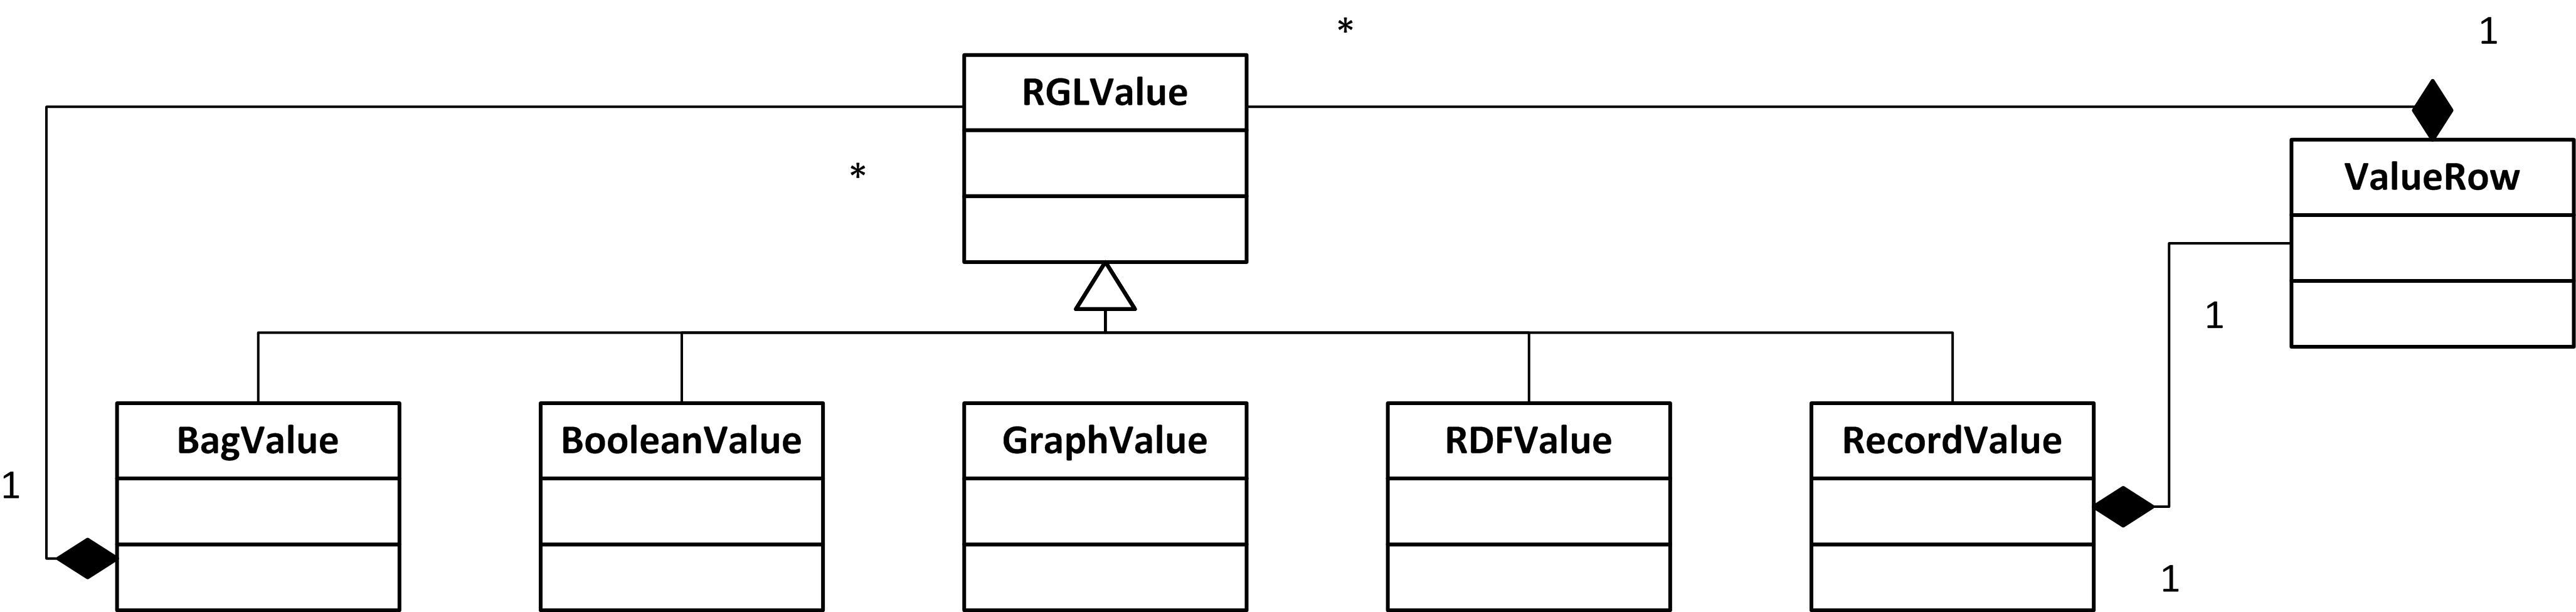
\includegraphics[scale=0.8]{storage/diagrams/RGLValues.png}
  \caption{Class diagram illustrating the RGL Values class hierarchy}
  \label{fig_rglValuesClassDiag}
\end{figure}

\begin{itemize}
	\item all data resides in just several database tables which makes the solution inefficient and hard to scale.
	\item all entities are stored in the same database tables and it is hard to distinguish between each other (eg. if one wants to query only one type of entities)
	\item the structure of the entities is not enforced by the database and has to be explicitly validated
	\item changing the structure of an entity may easily leave the db in an inconsistent state unless all existing entities are correctly migrated to the new structure
	\item most relational database access control mechanisms are based on tables and columns \cite{olson2008formal}. In this situation all entities reside in the same tables and therefore, it is hard to enforce access control on entity level.
\end{itemize}

The alternative approach that we propose is to map each entity type into separate JPA class which is named after the name of the entity. Table \ref{tbl:rgl2gpa} proposes a methodology to map RGL values to JPA entities.

\begin{table}[h]
    \begin{tabular}{ | l | l |}
    \hline
    \textbf{RGL} & \textbf{JPA}  \\ \hline
    RecordValue and its corresponding ValueRow & Class with multiple properties \textbf{*}  \\ \hline
    BagValue & Bag referring to a class representing\\ & the BagValue elements \\ \hline
    BooleanValue & Property of type boolean  \\ \hline
    RDFValue & Property of type string  \\ \hline
	GraphValue & Property of type string  \\ \hline
	
    \end{tabular}
     \caption{Table describing how RGL values are mapped to JPA}
    \label{tbl:rgl2gpa}
\end{table}

\textit{* JPA requires that the root element is a class and therefore, our solution requires and ensures that the root element of all entity types is a RecordValue. When this value is mapped to a JPA class the name of the class is the name of the entity type. Any nested RecordValues are mapped to JPA classes named after the name of the property of the ValueRow that points to them directly or indirectly in the case where the RecordValue is wrapped in a BagValue.}

This approach does not suffer from the problems of the first approach because each entity is stored in separate tables and also the database enforces the structure of the entities. However, it exposes several issues. The first issue is that each time the structure of an entity changes the JPA mapping information and the schema of the underling database has to be updated as well. Our solution to this problem is discussed in the next section. The second issue is that JPA requires that each entity has distinct id but RGL does not provide such term. We solve that problem by introducing an auto generated \textit{id} property for each JPA class which is made invisible to the client system (RDF Gears). Finally, JPA classes must have distinct names. We solve this problem by making sure that each user defined entity type has an unique name and also all fields within a record have distinct names as well. In order to make the names of the sub-entities (records) distinct we append to the front of their name the full path from the root JPA class separated by "\_".


\subsubsection{Representing RGL entities as Java objects}

JPA expects that each entity will have its own Java class representing it but our entities are virtual and there are no specific  classes that represent each of them. One solution to this problem would be to generate these classes on runtime. However, this approach is complex and error prone. Investigating the capabilities of different engines implementing the JPA specification relieved a promising feature in Hibernate called "Dynamic models" \cite{king2010hibernate}. It basically allows engineers to define the mapping logic into a special mapping XML file and on runtime present the entities in the form Java collections (Maps, Lists, Sets, etc.). Table \ref{tbl:rgl2java} shows how U-Sem entities can be expressed in terms of Java objects. This approach requires that every time when an entity is defined we have to build the XML mapping file and on runtime convert the RGL entities into Java collections and use Hibernate to store them into the database.

\begin{table}[h]
    \begin{tabular}{ | l | l |}
    \hline
    \textbf{RGL} & \textbf{Java}  \\ \hline
    RecordValue/ValueRow & Map with separate entries for each ValueRow \\ \hline
    BagValue & List  \\ \hline
    BooleanValue & boolean value  \\ \hline
    RDFValue & String value  \\ \hline
	GraphValue & String  value \\ \hline

    \end{tabular}
     \caption{Table describing how RGL values are mapped to Java objects}
    \label{tbl:rgl2java}
\end{table}
 
\subsubsection{Support for entity definition changes}

Another problem that has to be addressed concerns the dynamic nature of the entities. In our solution engineers have to be able to update the entity types whenever this is needed. Unfortunately, ORM frameworks are not good in dealing with such things. The problem is that whenever the entity type definitions changes not only the mapping XML file has to change but also the database schema. Hibernate provides a tool for table generation(hibernate.hbm2ddl.auto configuration option) but we were not able to find any documentation specifying how it works and what are its limitations. Additionally, we conducted experiments that reviled that this tool is not suitable for our situation. One of the problems is that when an entity is renamed then new set of tables is generated and the old ones are left behind. Therefore, in order to solve that problem reliably our solution provides functionality that is responsible to first update the mapping files and secondly update the schema of the database so that it is consistent with the new entity type definition. The algorithm for mapping JPA entities to tables in the relational database is the following:

\begin{itemize}
	\item A JPA class is mapped to a table with columns for each atomic property. 
	\item If a JPA property refers to another class then the target class is mapped recursively following the first step but its result table is also extended with an unique foreign key column pointing to the table representing the owner of the property.
	\item In the case of a JPA bag property referring to a class then the class is mapped recursively following the first step but its result table is also extended with a foreign key column pointing to the table representing the owner of the property.
\end{itemize}
 

\subsubsection{Querying}

The solution also has to provide approach for querying the stored entities. The query language has to be able to, first, allow engineers to write queries that identify entities or sub-entities to be updated or deleted. And, secondly, to enable them to filter, group and aggregate entities. 

In order to solve these requirements, we propose the use of JPQL \cite{linwood2010beginning}. It is a SQL like, high-level query language which omits details about the internal representation of the stored data \cite{linwood2010beginning}. It is the standard query language for JPA entities and is supported by most JPA providers including Hibernate. Its capabilities allow engineers to perform all the needed operations discussed above. Because of the direct mapping from RGL to JPA entities all possible JPQL query operations on the predefined entities are supported. The only exception is the additional \textit{id} field. In order to make it hidden for the engineers it is named "\$id\$" (Hibernate uses this notation to identify service fields) and using this field in queries is forbidden. Additional advantage of using JPQL comes from the fact that it is similar to SQL. In the current situation many of the engineers reported using SQL to implement data retrieval components and therefore, the transition to JPQL is likely to be easier.


\subsubsection{RDF Gears Components}
Finally, we have to define the RDF Gears components that are responsible to enable the engineer to configure and execute each type of the supported data operations. They are also responsible to automatically convert the data from RGL to the JPA compatible format and vice versa. The solution provides the following RDF Gears components:

\begin{itemize}
	\item \textit{Insert} - this component is responsible to insert an entity into the database. Engineers have to provide the name of the entity that has to be stored and the data itself.
	
	\item \textit{Query} - this component is responsible to enable engineers to query data. They have to configure the desired query and provide the required parameters for it.
	
	\item \textit{Delete} - this component is responsible to delete data from the database. Normally in JPA delete functionality relies on ids, but since we do not have this in the semantics of RGL we provide an alternative approach. In this case, engineers have to provide a query that selects all entities/sub-entities that have to be deleted. They are responsible to make sure that the query will produce only the needed results.
	
	\item \textit{Update} - this component is responsible to enable engineers to update entities or part of them. Like the delete operation, updates in JPA are also based on ids. So we approached the problem similarly. Engineers provide a query that selects all entities (sub entities) that will be updated. They have to also state the fields of the selected entities that have to be updated and provide the values. The system distincts between two types of updates. The first one is replacing the value of a field (basic type, record or bag). The second one is aimed for appending an element to a bag.
\end{itemize}

\subsection{Multi-engineer support}

The second challenge that we have to solve is to enable multiple engineers to work with the solution simultaneously. In order to support that we have to investigate the following issues: how to organize the database, how to enable collaboration and how to manage access control.

\subsubsection{Database Organization}

Designing the solution we considered two possible approaches for establishing the database organization:

\begin{itemize}

\item \textit{Independent Databases} - in this approach engineers share only the hardware (server). Each of them operates on an independent database instance. This approach provides good data isolation and security but the set-up and maintenance costs are significantly increased as a result of the multiple database instances. Additionally, collaboration between engineers is problematic because of the difficulty to execute queries on data that resides over several databases.  
	
\item \textit{Shared Database} - in this approach, all engineers share the same database instance. This approach seems better for U-Sem because it does not suffer from the data querying problem discussed above and also reduces the set-up and maintenance costs which is one of the main goals of this work. The fact that all data resides in a single database, however, requires the solution to provide strong mechanism that ensures isolation between engineers' data but also define ways for data level interaction which is covered in next section.

\end{itemize}


\subsubsection{Collaboration}
The ability for engineers building workflows to collaborate and reuse each others data is essential \cite{lu2009collaborative}. Choosing the Shared Database organization makes it easy for engineers to work with the data of the others. However, there are several issues that have to be discussed and addressed:

\begin{itemize}

	\item \textit{privacy} - sometimes engineers might not want others to use their data. This might be because of privacy issues or there might be entities that are not designed to be shared. Therefore, engineers want to limit the access to their data. For example they might only allow others to read the data but not to modify it. Therefore, when the engineer defines an entity he should be able to specify its sharing options which are enforced by the solution. This issue is further discussed in the \textit{Access Control} section below.
	 
	\item \textit{semantics and structure of shared data} - the solution can further assist engineers that want to reuse shared data by providing information about its structure and semantics. Implementing such functionality will save them a lot of time since otherwise this information has to be communicated by other means which may require a lot of time.
	
	\item \textit{entities mutation} - providing multi-engineer support introduces the problem with the consistency. By design entities can change and evolve over time. Therefore the system should prevent any inconsistent results produced if the structure changes at the time a workflow is executed. Our solution deals with that problem using database transactions \cite{gray1981transaction}. All data operations are executed in transactions which temporary lock the tables for modification. As a result, the changing request will wait for the tables to be released before applying the updates to the database schema.
\end{itemize}


\subsubsection{Access control}

As mentioned above engineers have to be able to control the access to their data. The storage abstraction discussed in this chapter enables engineers to insert, update, delete and query data. Therefore, we propose an extension to the abstraction that will enable engineers to also control the execution of these operations on their data by other engineers. The basic idea is that when engineers define their entities they can also specify how their data can be accessed by others.

The hierarchical structure of the entities expressed in RGL is very similar to XML and it can be, indeed, expressed as XML \cite{feliksik2011}. Therefore, adopting an approach used for establishing access control for XML document systems seems to be feasible. Inspired by the work of \cite{wu2005access} we propose a fine grained access control framework for RGL entities. It is based on access control rules that are defined by the engineers that build a particular entity. This rules are responsible to grand access to other engineers for entities or parts of entities. They can be presented as triples G $\times$ O $\times$ R where: 
\begin{itemize}
	\item g $\in$ G is the grandee it can be a user or user group that this rule targets.
	\item o $\in$ O is the object that the rule applies for. It can be entity or parts of entity which as discussed in previous sections are identified by expressions constituting the full path from the root of the entity separated by "\_".  
	\item r $\in$ R is the operation that is granted: insert, update, delete or query.
\end{itemize}

Once we have the rules we have to identify the granularity (which parts of the entities they can be applied to). It can vary from entire entities to the level of basic RGL values. Choosing the entity level of granularity seems to be too sparse since it does not support use-cases where engineers what to share only parts of the entities and protect the rest. On the other hand, providing access control for every single element in an entity is likely to make the user interface too complicated and thus, harder to configure. Therefore, we propose to use an intermediate level of granularity which provides a reasonable flexibility and also can be easily configured and implemented. 

The approach allows engineers to apply the access rules for each entity and  also for all records in the entity hierarchy. If no access rules are specified then the elements are considered private and accessible only by their owner. The access policy for the other RGL elements is the access policy defined for the first parent record in the hierarchy or if such does not exist - the policy for the entire entity. In order to save engineers time when the same rules have to be applied for the entire entity hierarchy or parts of it the approach also defines an inheritance mechanism. By default the access rules defined for the entity are inherited for the entire structure of the entity. Engineers, however, may choose to override this policy for particular records. In that case the new rules are automatically inherited in the sub-hierarchy where the same mechanism is applied recursively.


\paragraph{Implementation approach}

The solution has to be able to enforce the sharing policy of the entities and make sure that data is not accessed illegally. Therefore, the solution provides access control functionality that is responsible to enforce this policies. Basically, JPA is not good at doing this, it does not provide any access control functionality out of the box. Therefore, there are two possible places to put the access control logic. 

\begin{itemize}
	\item \textit{Above JPA} - our solution wraps around the JPA engine and thus, we can control all the requests that it receives. We can provide functionality that validates if the user has the needed permissions to execute that functionality. However, from engineering perspective doing this will be hard since JPA (JPQL) allows engineers to construct relatively complex queries and building a functionality that pareses these queries is not a trivial job to do and significantly increases the risk of security wholes.
	
	\item \textit{Database level} - the second option is to make the database enforce the security policies. We think that this approach is much easier because databases already provide well established access control mechanisms \cite{olson2008formal}. The only think that we have do is to apply the security policy using the database language every time an entity is created or modified. As a result, the database will stop the JPA framework accessing data that it is not authorised to access.
	
	
Most SQL databases like MySQL\footnote{MySQL - http://www.mysql.com/} enable engineers to define access control rules on table level. The proposed approach in this chapter defines that each entity is mapped to a database table and each record within the entity hierarchy is also mapped to a distinct table. Therefore, the system must only translate the access control rules of U-Sem to the rules supported by the database.
\end{itemize}


\subsection{Components with side effects in RDF Gears}

In the Section \ref{sec:backRDFGears} we discuss how RDF Gears evaluates and optimizes workflows which is based on the assumption that components do not have side effects. However, with the introduction of the new data manipulation components this assumption is no longer correct. Therefore, the engine may no longer perform its tasks correctly. The trivial approach for solving this problem would be to simply remove all these optimizations but this is not a good idea because this will reduce the efficiency of the engine. Therefore, we propose an alternative approach which aims to make the engine perform correctly but also keep the efficiency.

Currently the workflow definition language of RDF Gears does not support any conditional branching \cite{feliksik2011} and therefore, all components are expected to be executed. However, for efficiency reasons it executes only the components that contribute to the final result which in the basic case is the output node and its (indirect) dependencies. Our solution extends this idea and states that the components that contribute to the final result are also the components that have side effects and their (indirect) dependencies. Our solution consists of the following steps:

\begin{itemize}
	\item extend the function description notation of RDF Gears so that the engine knows if a component has side effects or not.
	\item on execution time when the data structure containing the components that are going to be executed is built we also include all components that have side effects and recursively all the components that they depend on.
	\item we perform all the optimizations to the output node (as it is currently done) as well as to all components with side effects. 
	\item when the workflow is executed we execute it for the output node and for all components with side effects. The caching mechanism prevents components to execute several times. The output of the workflow is still the output of the output node.
\end{itemize}

These steps ensure that all components with side effects are executed and the execution is efficient because all the optimizations are applied.

\subsection{Integration with the plug-in environment}

We also designed an additional feature that aims to save time to engineers. Its idea is to integrate the data management feature with the plug-in environment feature. The benefit from this feature covers the situation when engineers create a certain kind of user modelling service which requires data storage or retrieval and bundle it into a plug-in. It requires some entity definitions in order to work and therefore, every time this plug-in is deployed on a server the engineers have to manually define the needed entities through the user interface. Obviously, this operation may cost significant time and is also error prone. Additionally, the problem becomes severe when an engineers wants to use a shared plug-in produced by someone else. In this case the two engineers need a way to somehow exchange the entity definitions.

In order to solve that problem we have devised a mechanism that can deal with this issue automatically and thus save time to the engineers. Each entity definition is stored in an XML file in the file system. Therefore, every time an engineer creates an entity definition he can export it as an XML file. Then, he can include this file in the plug-in and register it within the plug-in context. When this plug-in is installed the system automatically detects the presence of these entity definitions and installs them automatically so that the functionality of the plug-in can be used right away without any need for configuration.

\section{Architecture}
\label{sec:architectureStorage}

Based on the approach devised in the previous section we designed the software architecture for the \textit{Data Management} feature of U-Sem. In this section we present the description of the proposed architecture. Following the same documentation approach discussed in Section \ref{sec:architecturePlugin}, we provide a set of interrelated views, which collectively illustrate the functional and non-functional features of the system from different perspectives and demonstrate that it meets the requirements. 


\subsection{Functional View}

In this section we present he functional structure of the solution which includes the key functional elements, their responsibilities, the interfaces they expose, and the interactions between them \cite{rozanski2011software}. All these together demonstrate how the system will perform the required functions. All components that build up the data management feature can be classified in three layers. This organization is illustrated in Figure \ref{fig:storageLayers} and consists of the following layers:

\begin{figure}[h!]
  \centering
  	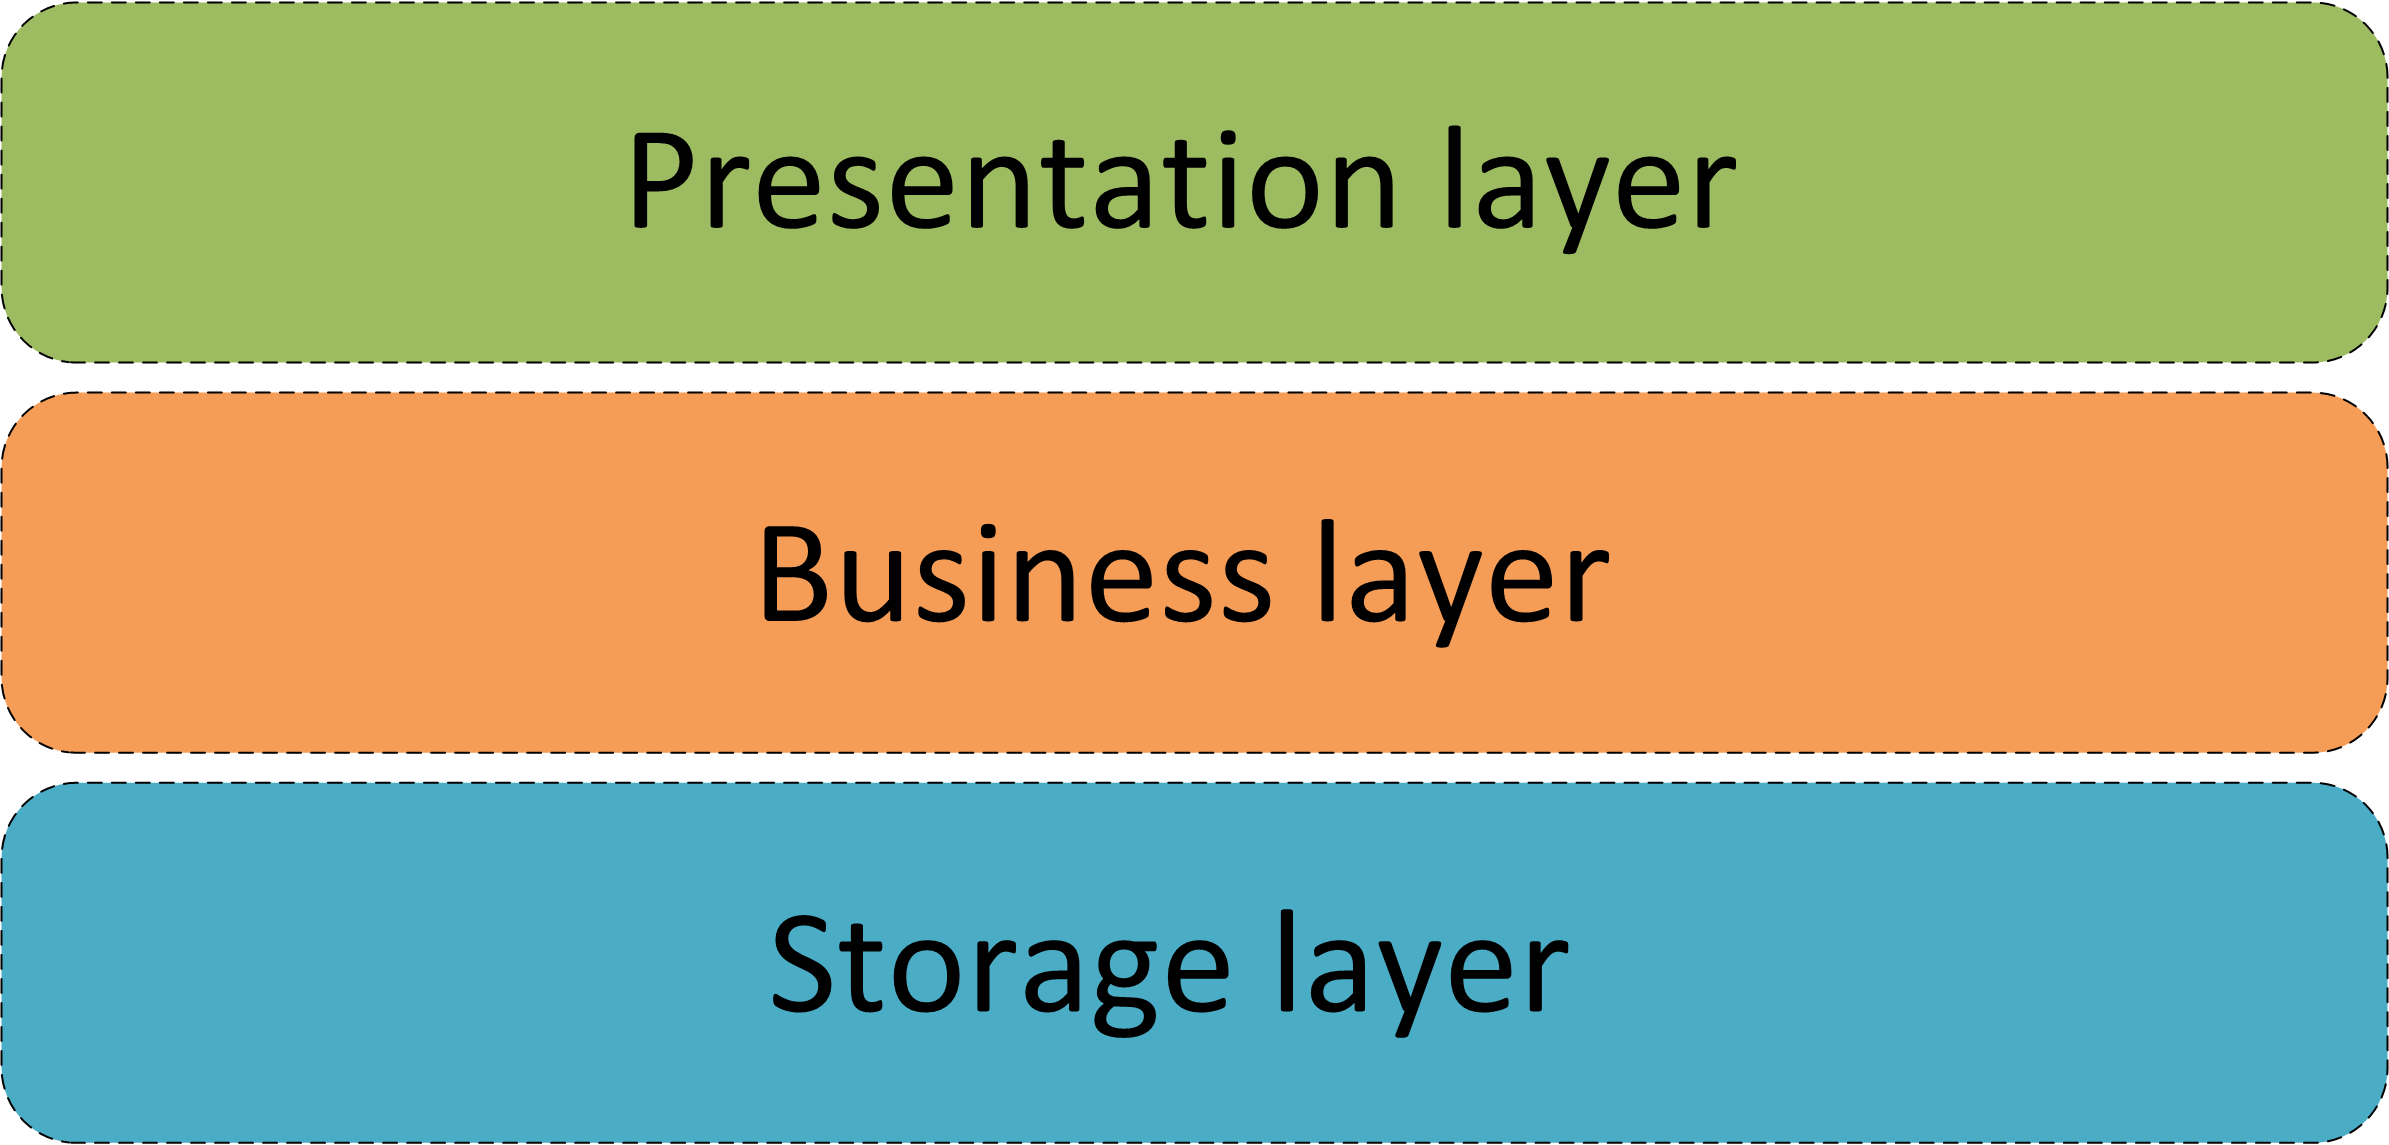
\includegraphics[scale=0.6]{storage/functional/layers.png}
  \caption{Layer organization of the feature}
  \label{fig:storageLayers}
\end{figure}

\begin{itemize}
	\item \textit{Presentation layer} - this layer consists of all functional components that are responsible to provide the user interface that enables engineers to define and manipulate persistent data.
	
	\item \textit{Business layer} provides functionality for defining the structure and semantics of the data and manipulating the actual data. The functional components that build this layer are responsible to enforce the security and privacy policies of the system.
	
	\item \textit{Storage layer } is responsible to provide storage functionality for storing the entity definitions, the hibernate mappings and the actual data.
\end{itemize}

\subsubsection{High-level component organization}
This section describes the internal structure of the layers and identifies the high level components that build up the feature. Figure \ref{fig:storageFuncMain} illustrates this organization. It shows how the high-level components are organized into the layers and the way they depend on each other. We have identified the following high level components:

\begin{figure}[h!]
  \centering
  	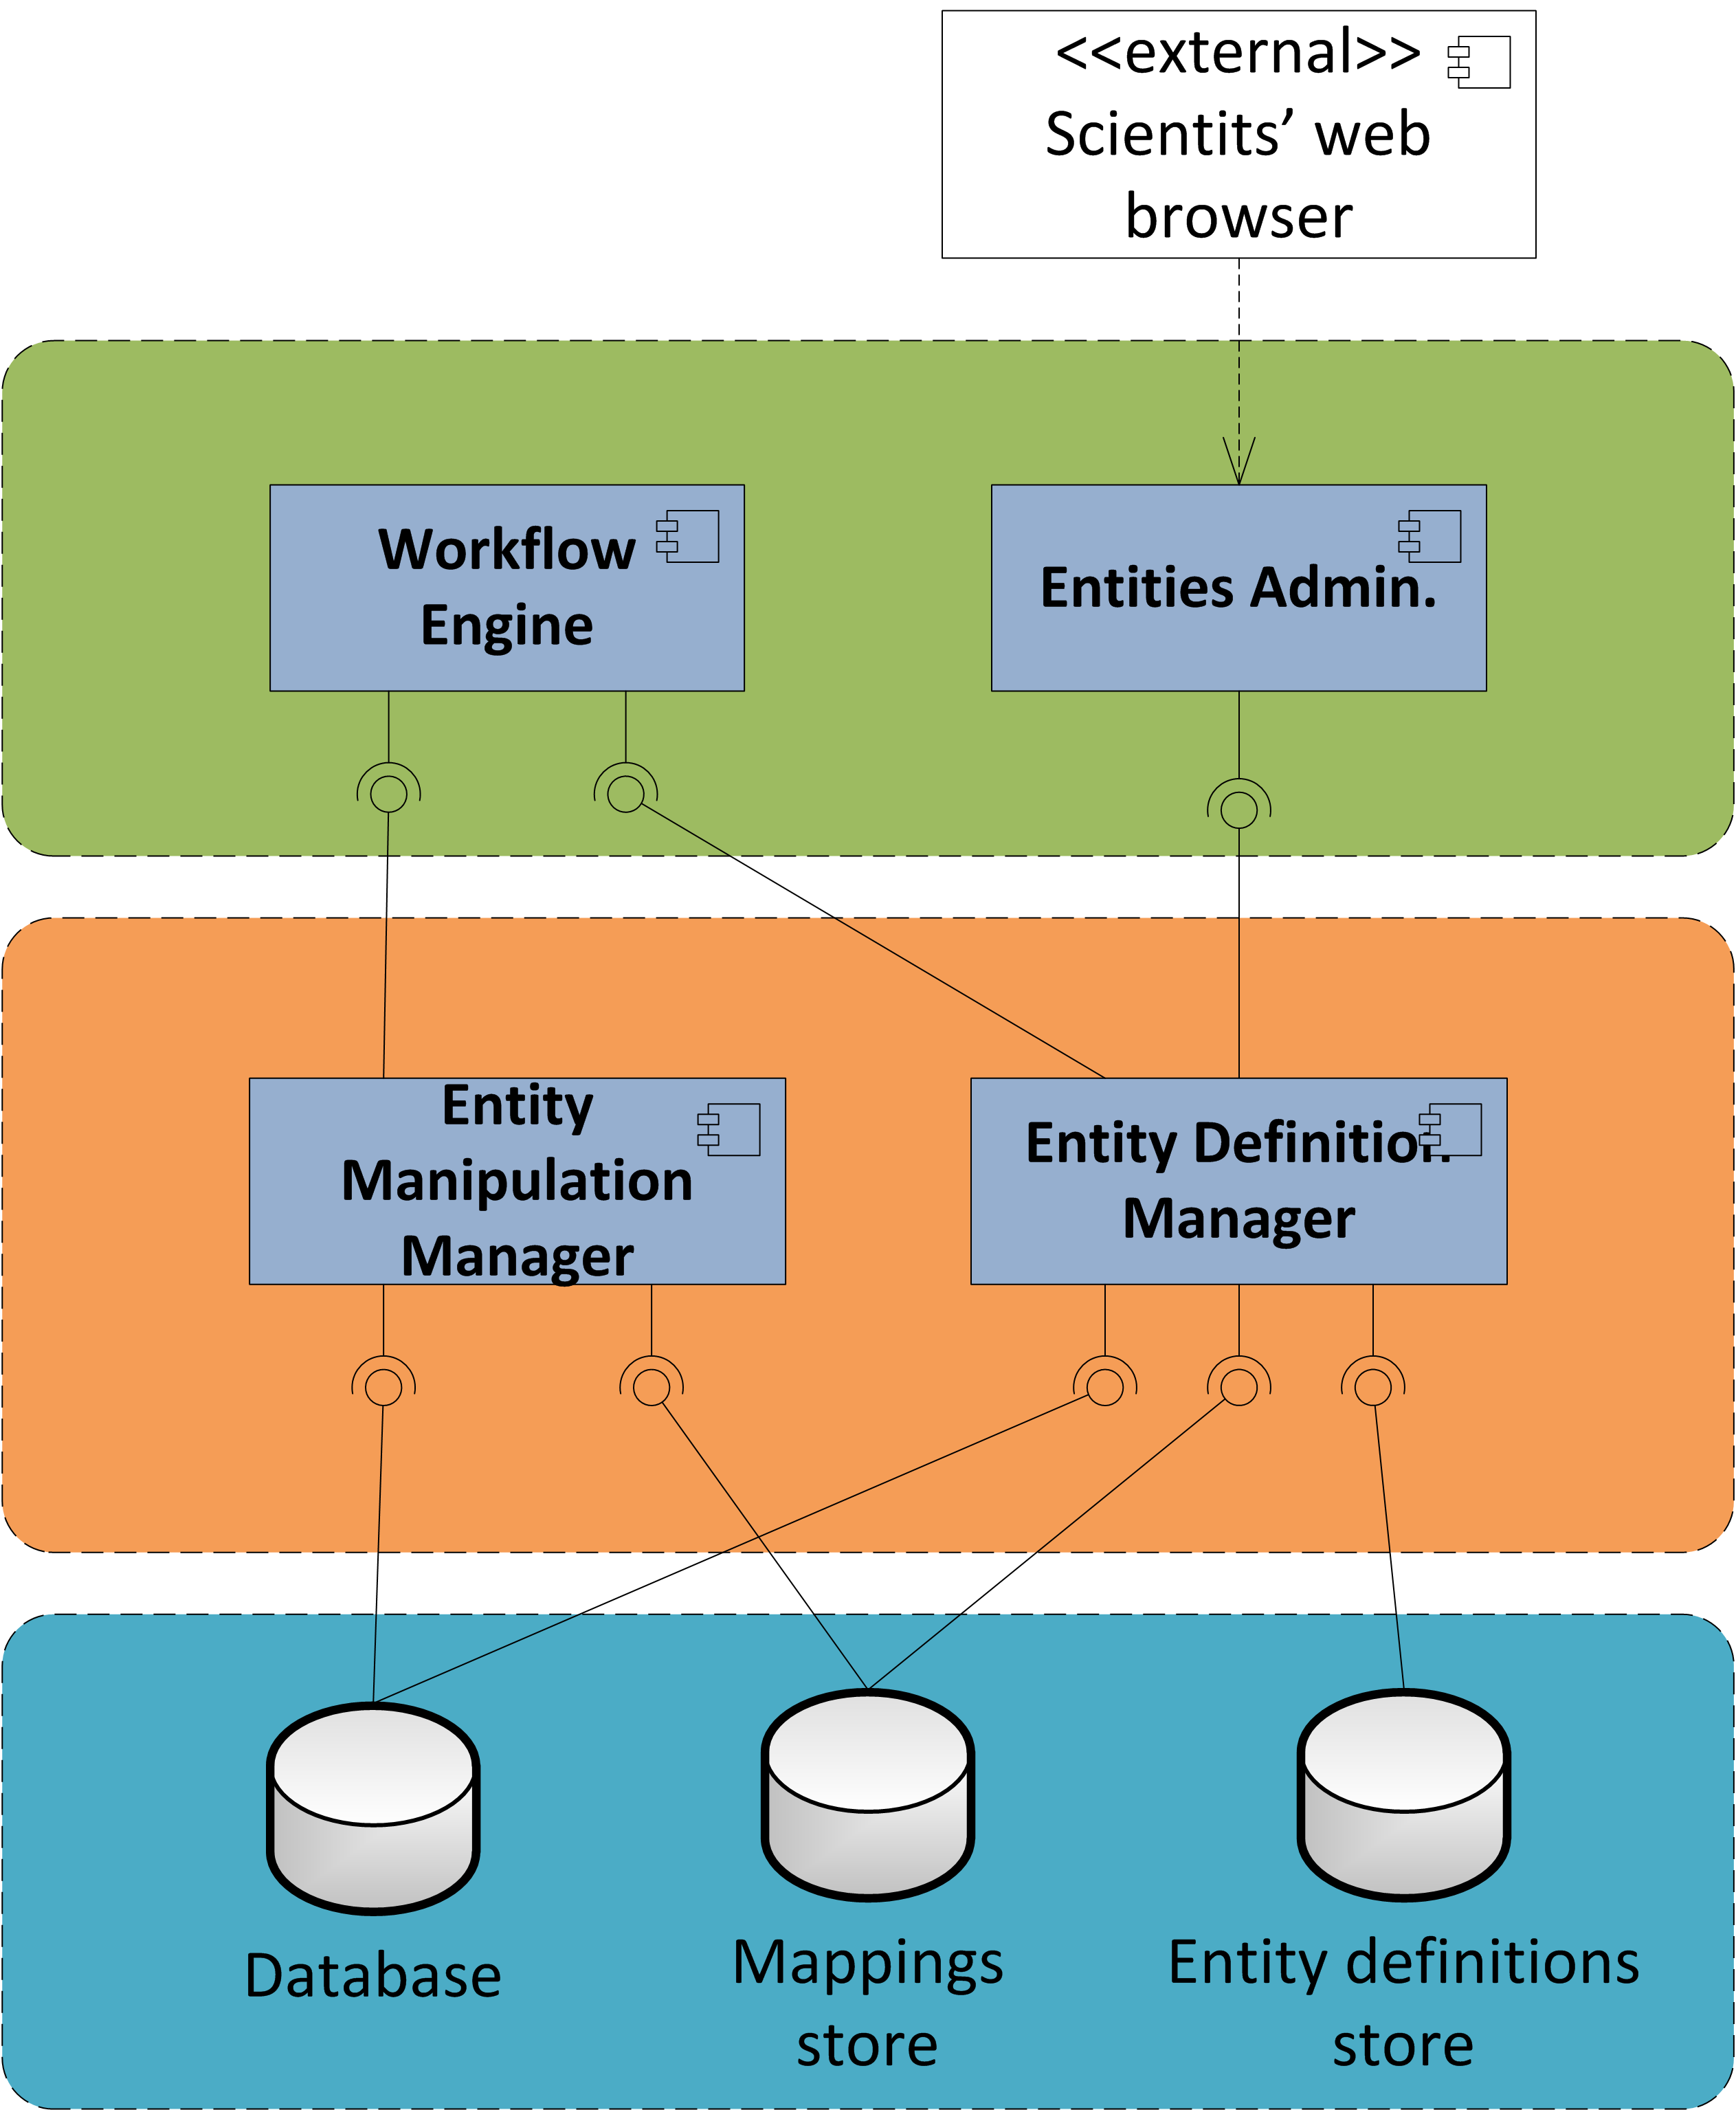
\includegraphics[scale=0.75]{storage/functional/func_main.png}
  \caption{Component diagram illustrating the high level functional organization of the feature }
  \label{fig:storageFuncMain}
\end{figure}

\begin{itemize}
	
	\item \textit{Entity definitions store} - Provides functionality for storing the data describing the entity definitions. 
		
	\item \textit{Mappings store} - Provides functionality for storing the data defining how entities are mapped to the database.  
	
	\item \textit{Database} - Relational database that is responsible to store and provide access to the actual data.
	
	\item \textit{Entity Definition Manager} - this component is responsible to provide an API which enables high level components to manipulate entity definitions. It is responsible to handle the storage the entity definitions, create the mappings that state how the data is mapped to the database and also prepare the database (create required tables and set access permissions) for working with the defined entities. Further decomposition of this component is provided in the next sections.
		
	\item \textit{Entity Manipulation Manager} - this component is responsible to provide the functionality needed for manipulating data based on the previously created entity definitions. It provides an API which enables high level components to perform storing, updating, deleting and querying of data. Further decomposition of this component is provided in the next sections.
	
	\item \textit{Entities Admin.} - responsible to provide the system`s endpoints (user interface) that enable engineers to define and manage their entities. Further decomposition of this component is provided in the next section.

	\item \textit{Workflow Engine} - uses the APIs provided by the \textit{Entity Definition Manager} and the \textit{Entity Manipulation Manager} to enable engineers define data entities and create services that manipulate persistent data. During the workflow configuration phase it uses the APIs in order to obtain the list of already defined entities (their structure and their semantics) assisting engineers to easily define workflows that require data manipulation. During the workflow execution phase it uses the APIs to execute the defined data operations.
\end{itemize}

\subsubsection{Entities administration}
This section defines the functional decomposition of the Entities administration component which is illustrated on figure \ref{fig:storageFuncAdmin}. It consists of the following components:

\begin{figure}[h!]
  \centering
  	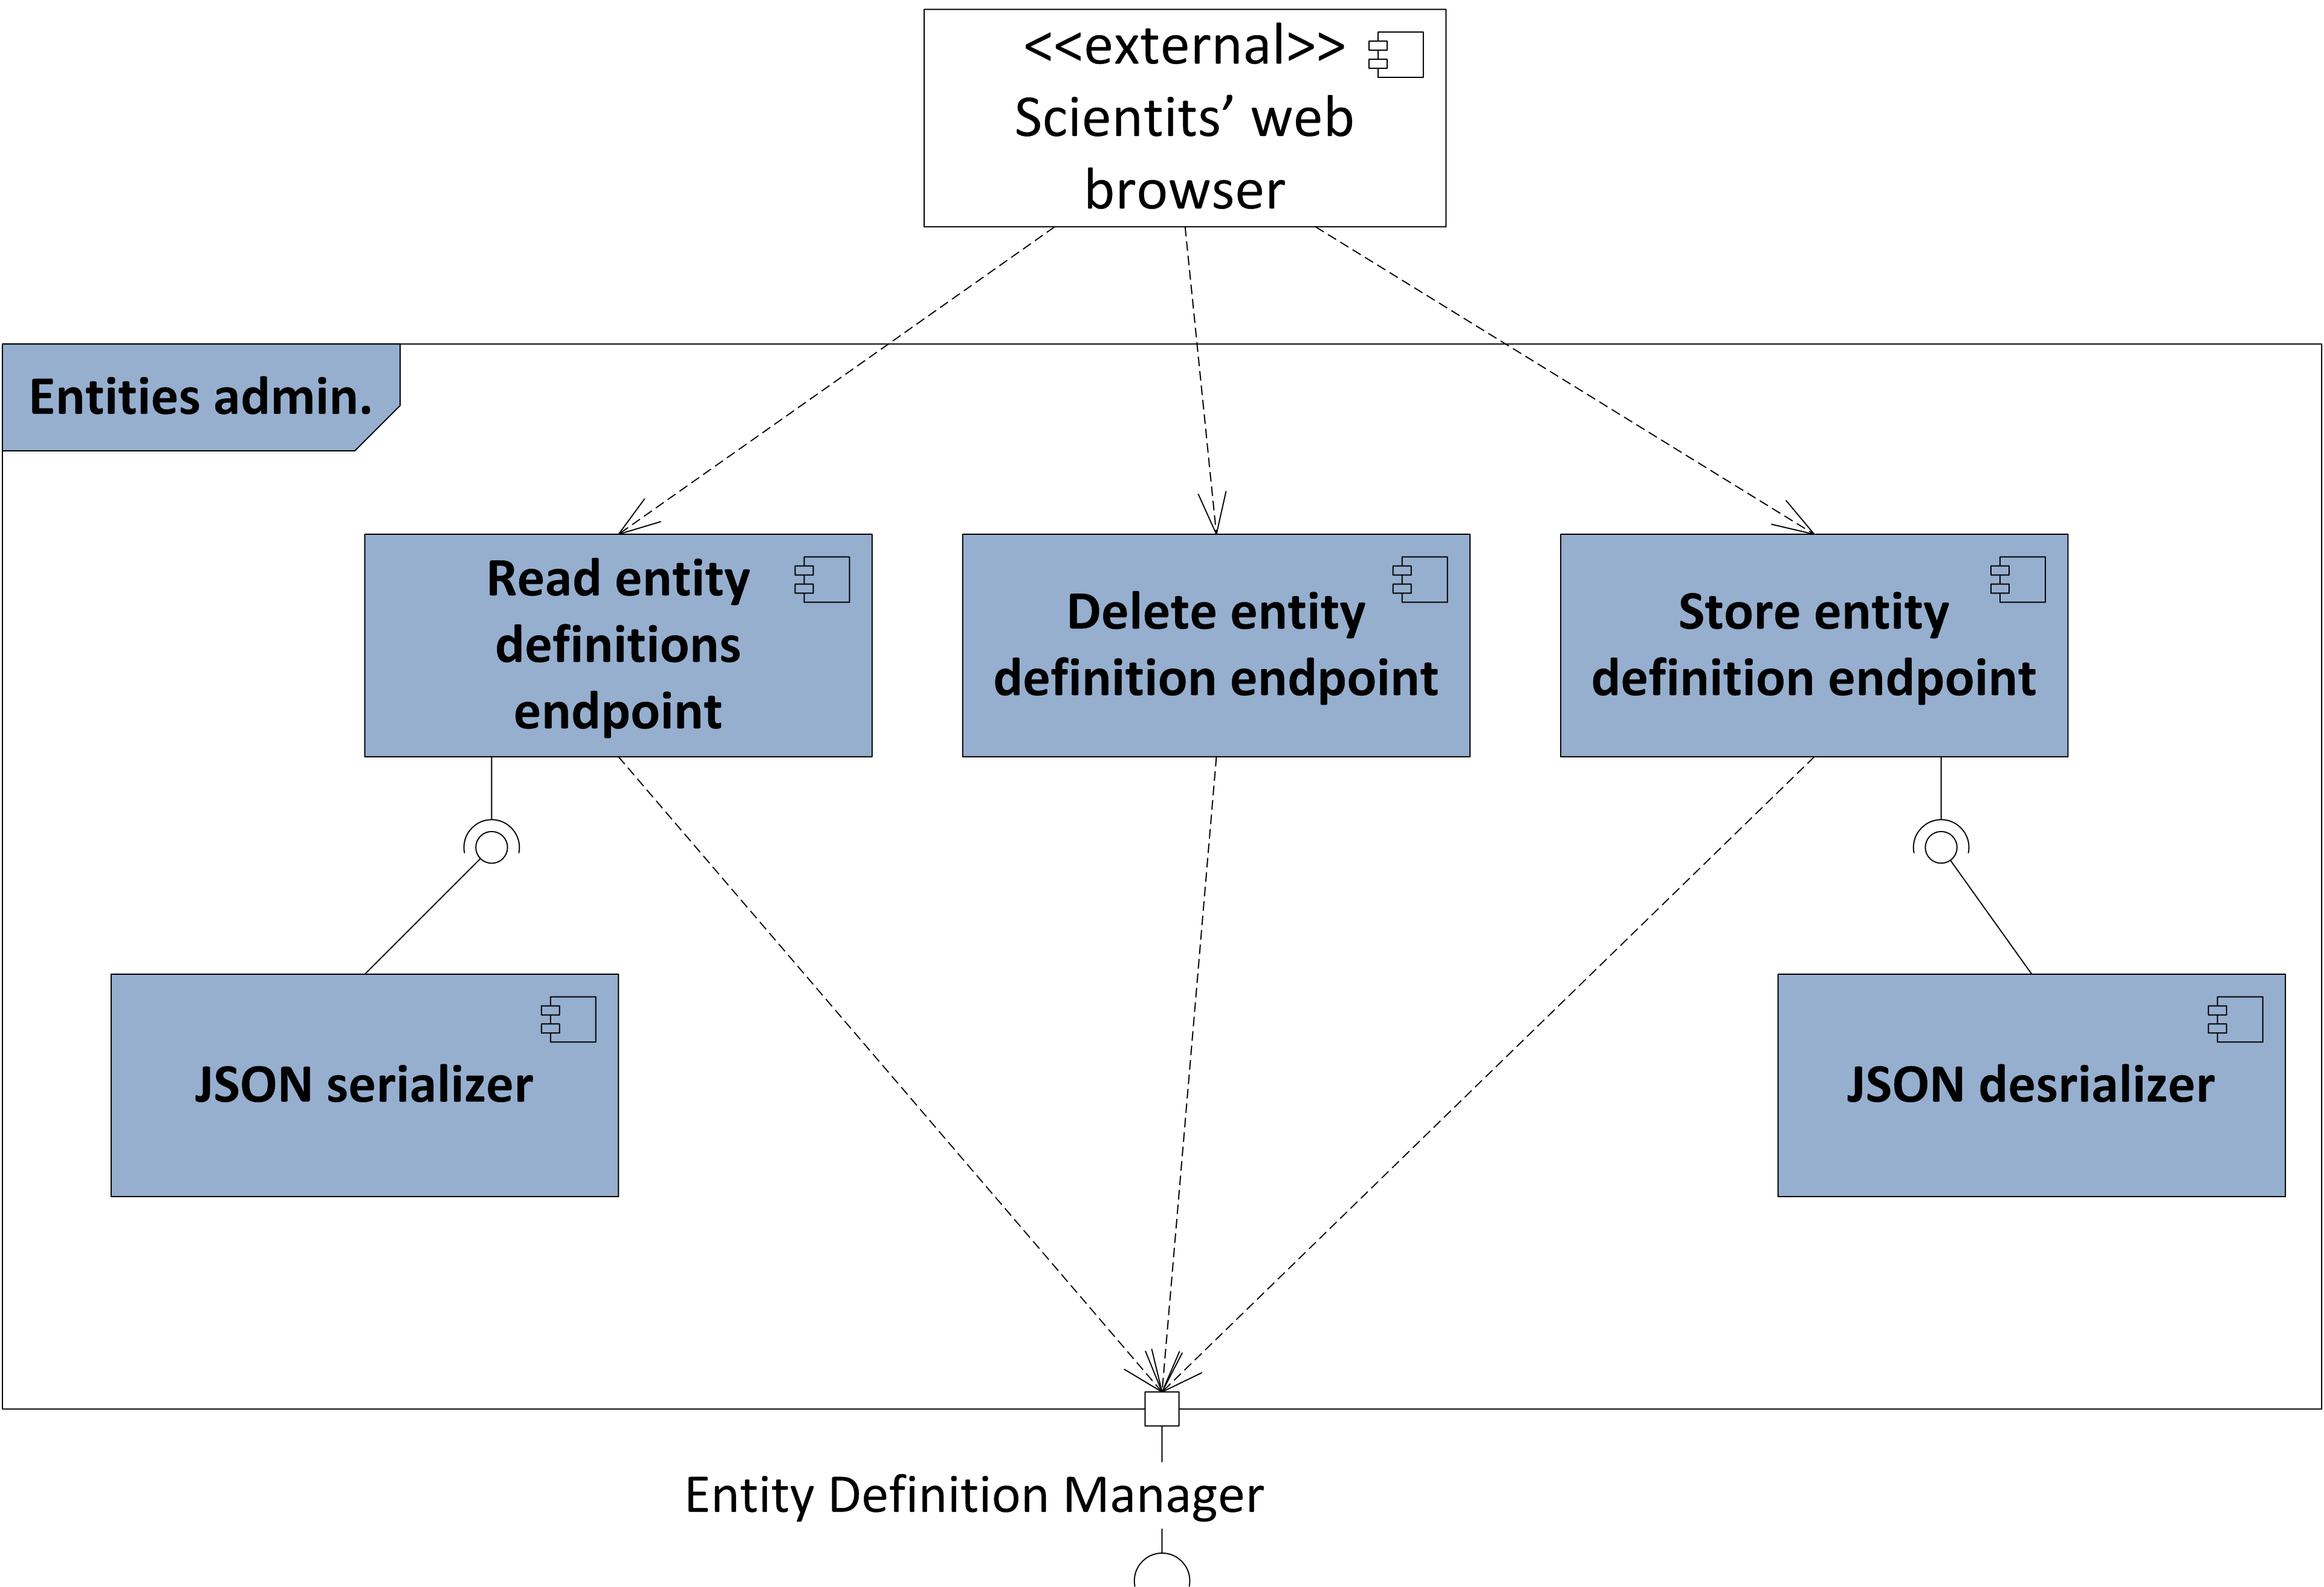
\includegraphics[scale=0.75]{storage/functional/func_admin.png}
  \caption{Functional decomposition of the Entities admin. module}
  \label{fig:storageFuncAdmin}
\end{figure}

\begin{itemize}
	\item \textit{Read entity definitions endpoint} - This component provides the user interface needed for browsing the already defined entities.
	
	\item \textit{Delete entity definition endpoint} - This component provides the user interface needed for removing a selected entity definition.
	 
	\item \textit{Store entity definition endpoint} - This component provides the user interface needed for creating new or updating existing entity definitions.
	
	\item \textit{JSON de/serializer} - Since data in the user interface is presented in the form of JSON. This components are responsible to convert the entity definitions from/to JSON format.
	
\end{itemize}

\subsubsection{Entity Definition Manager}
This component is responsible to provide API which can be used by presentation layer components in order to manage the entity definitions. Figure \ref{fig:storageFuncAccess} shows the functional decomposition of this module. It consists of the following components:

\begin{itemize}
	\item \textit{Facade} - this component provides the API for manipulating the entity definitions.
	
	\item \textit{DB Schema persister} - this component is responsible to make sure the database schema is always corresponding to the entity definitions. Any time the entities are changed the database schema is updated. Additionally, this component also defines the access permissions for each access table based on the access rules defined by the engineers.
	
	\item \textit{Hibernate mappings persister} - this component is responsible to construct the mappings that define how data is mapped and stored in the database. Since we are using Hibernate, this information is created and stored as "hbm" files. Every time the entity definitions are changed the mappings are updated as well.
	
	\item \textit{Entity definition persister} - this component is responsible to store and retrieve the entity definitions. It provides a level of abstraction over the way the definitions are stored. As a result, this will be the only component that is affected in case any change of the place and format of the data is required. The default implementation of this component depends on the \textit{XML Serializer} component for storage in XML files.
	
	\item \textit{XML Serializer} -  this component is responsible to define the way entity definitions are stored and retrieved from XML files.
\end{itemize}


\begin{figure}[h!]
  \centering
  	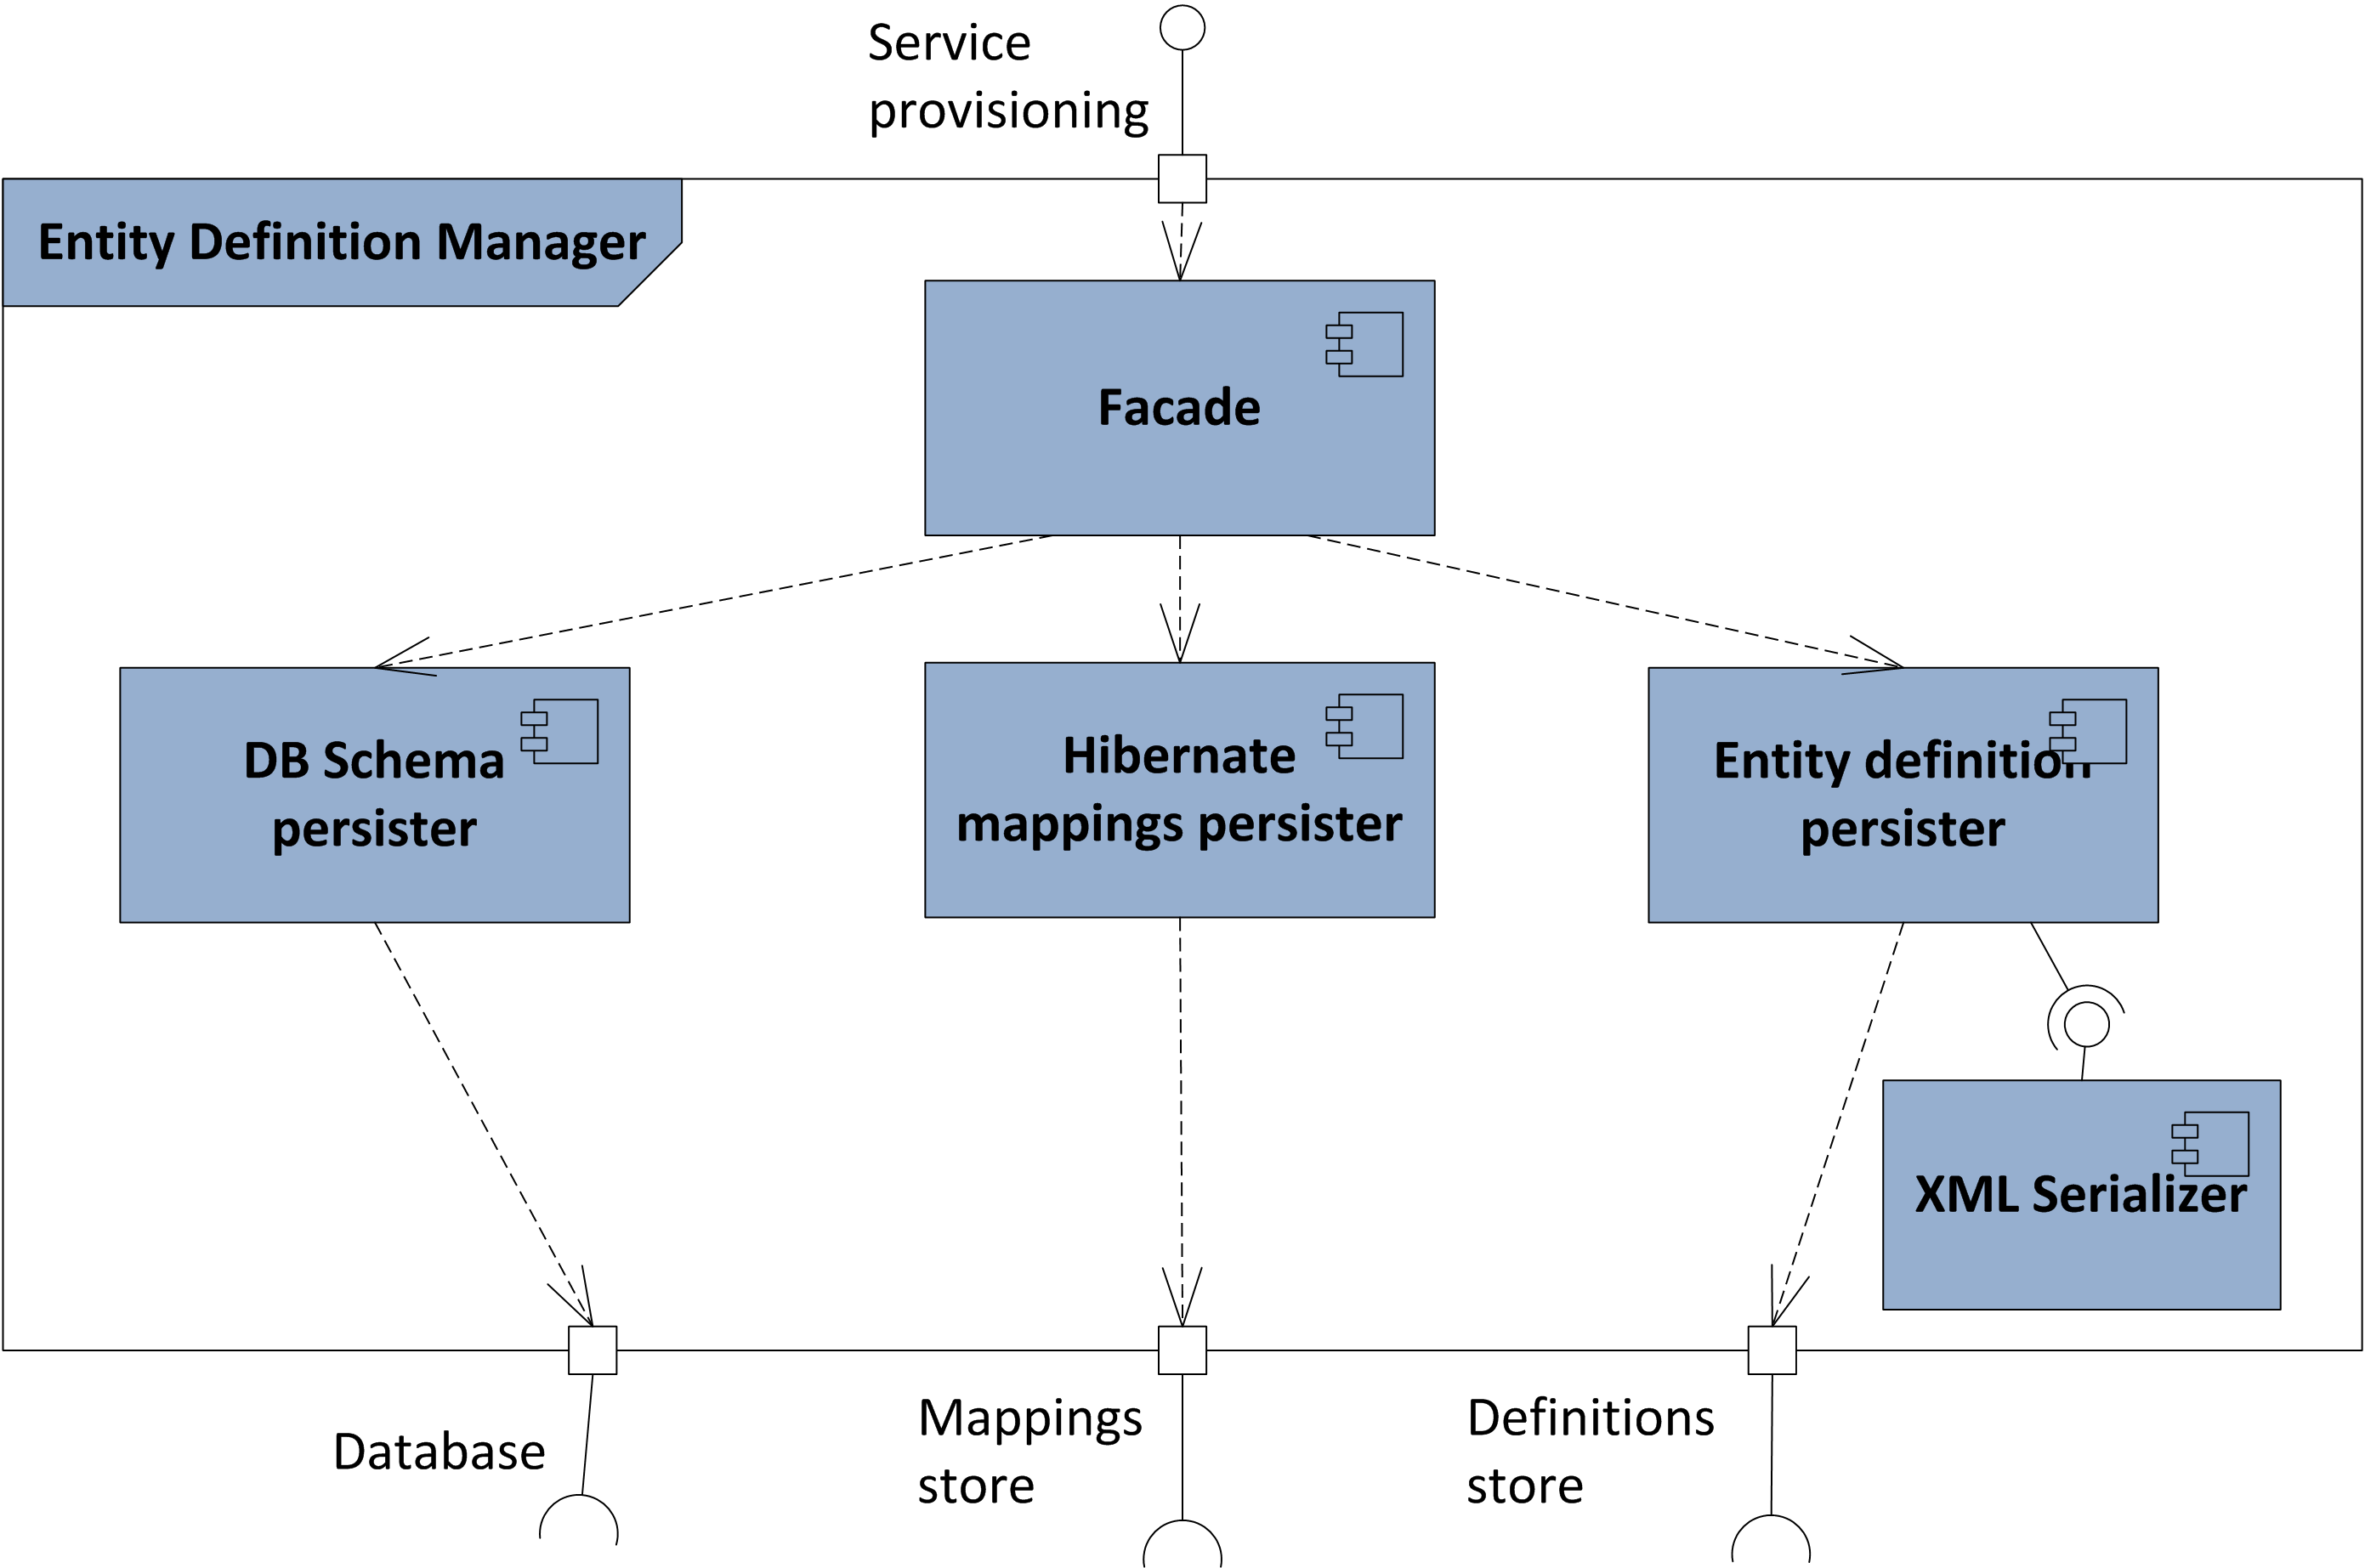
\includegraphics[scale=0.9]{storage/functional/func_access.png}
  \caption{Functional decomposition of the Entities Definition Manager module}
  \label{fig:storageFuncAccess}
\end{figure}

\subsubsection{Entity Manipulation Manager}

This component is responsible to provide API which can be used by presentation layer components in order to perform data manipulation operations over the already defined entities. Figure \ref{fig:storageFuncManip} shows the functional decomposition of this module. It consists of the following components:


\begin{itemize}
	\item \textit{Data manipulation manager} - This component provides the API for data manipulation. It manages the communication with the Hibernate framework and is responsible to start/stop the framework and monitor its life cycle. It also acts as a level of abstraction over the framework and in case any change in future is required, this will limit the number of affected components.
	
	\item \textit{Properties provider} - This component keeps track of all common and user related options that are required for the correct operation of the Hibernate framework. The main properties this component is responsible to provide are the database login configuration for each engineer. It has to make sure that each request to the database is executed with the correct database user so that the database can handle the access control properly.
	
	\item \textit{Mappings provider} - This component is responsible to provide the "hbm" mapping files that are required by the Hibernate framework so that it can work with the defined entities.
	
	\item \textit{Hibernate} - This component represents the Hibernate framework which is responsible to perform the actual interaction with the database in order to serve the data manipulation requests.  
\end{itemize}

\begin{figure}[h!]
  \centering
  	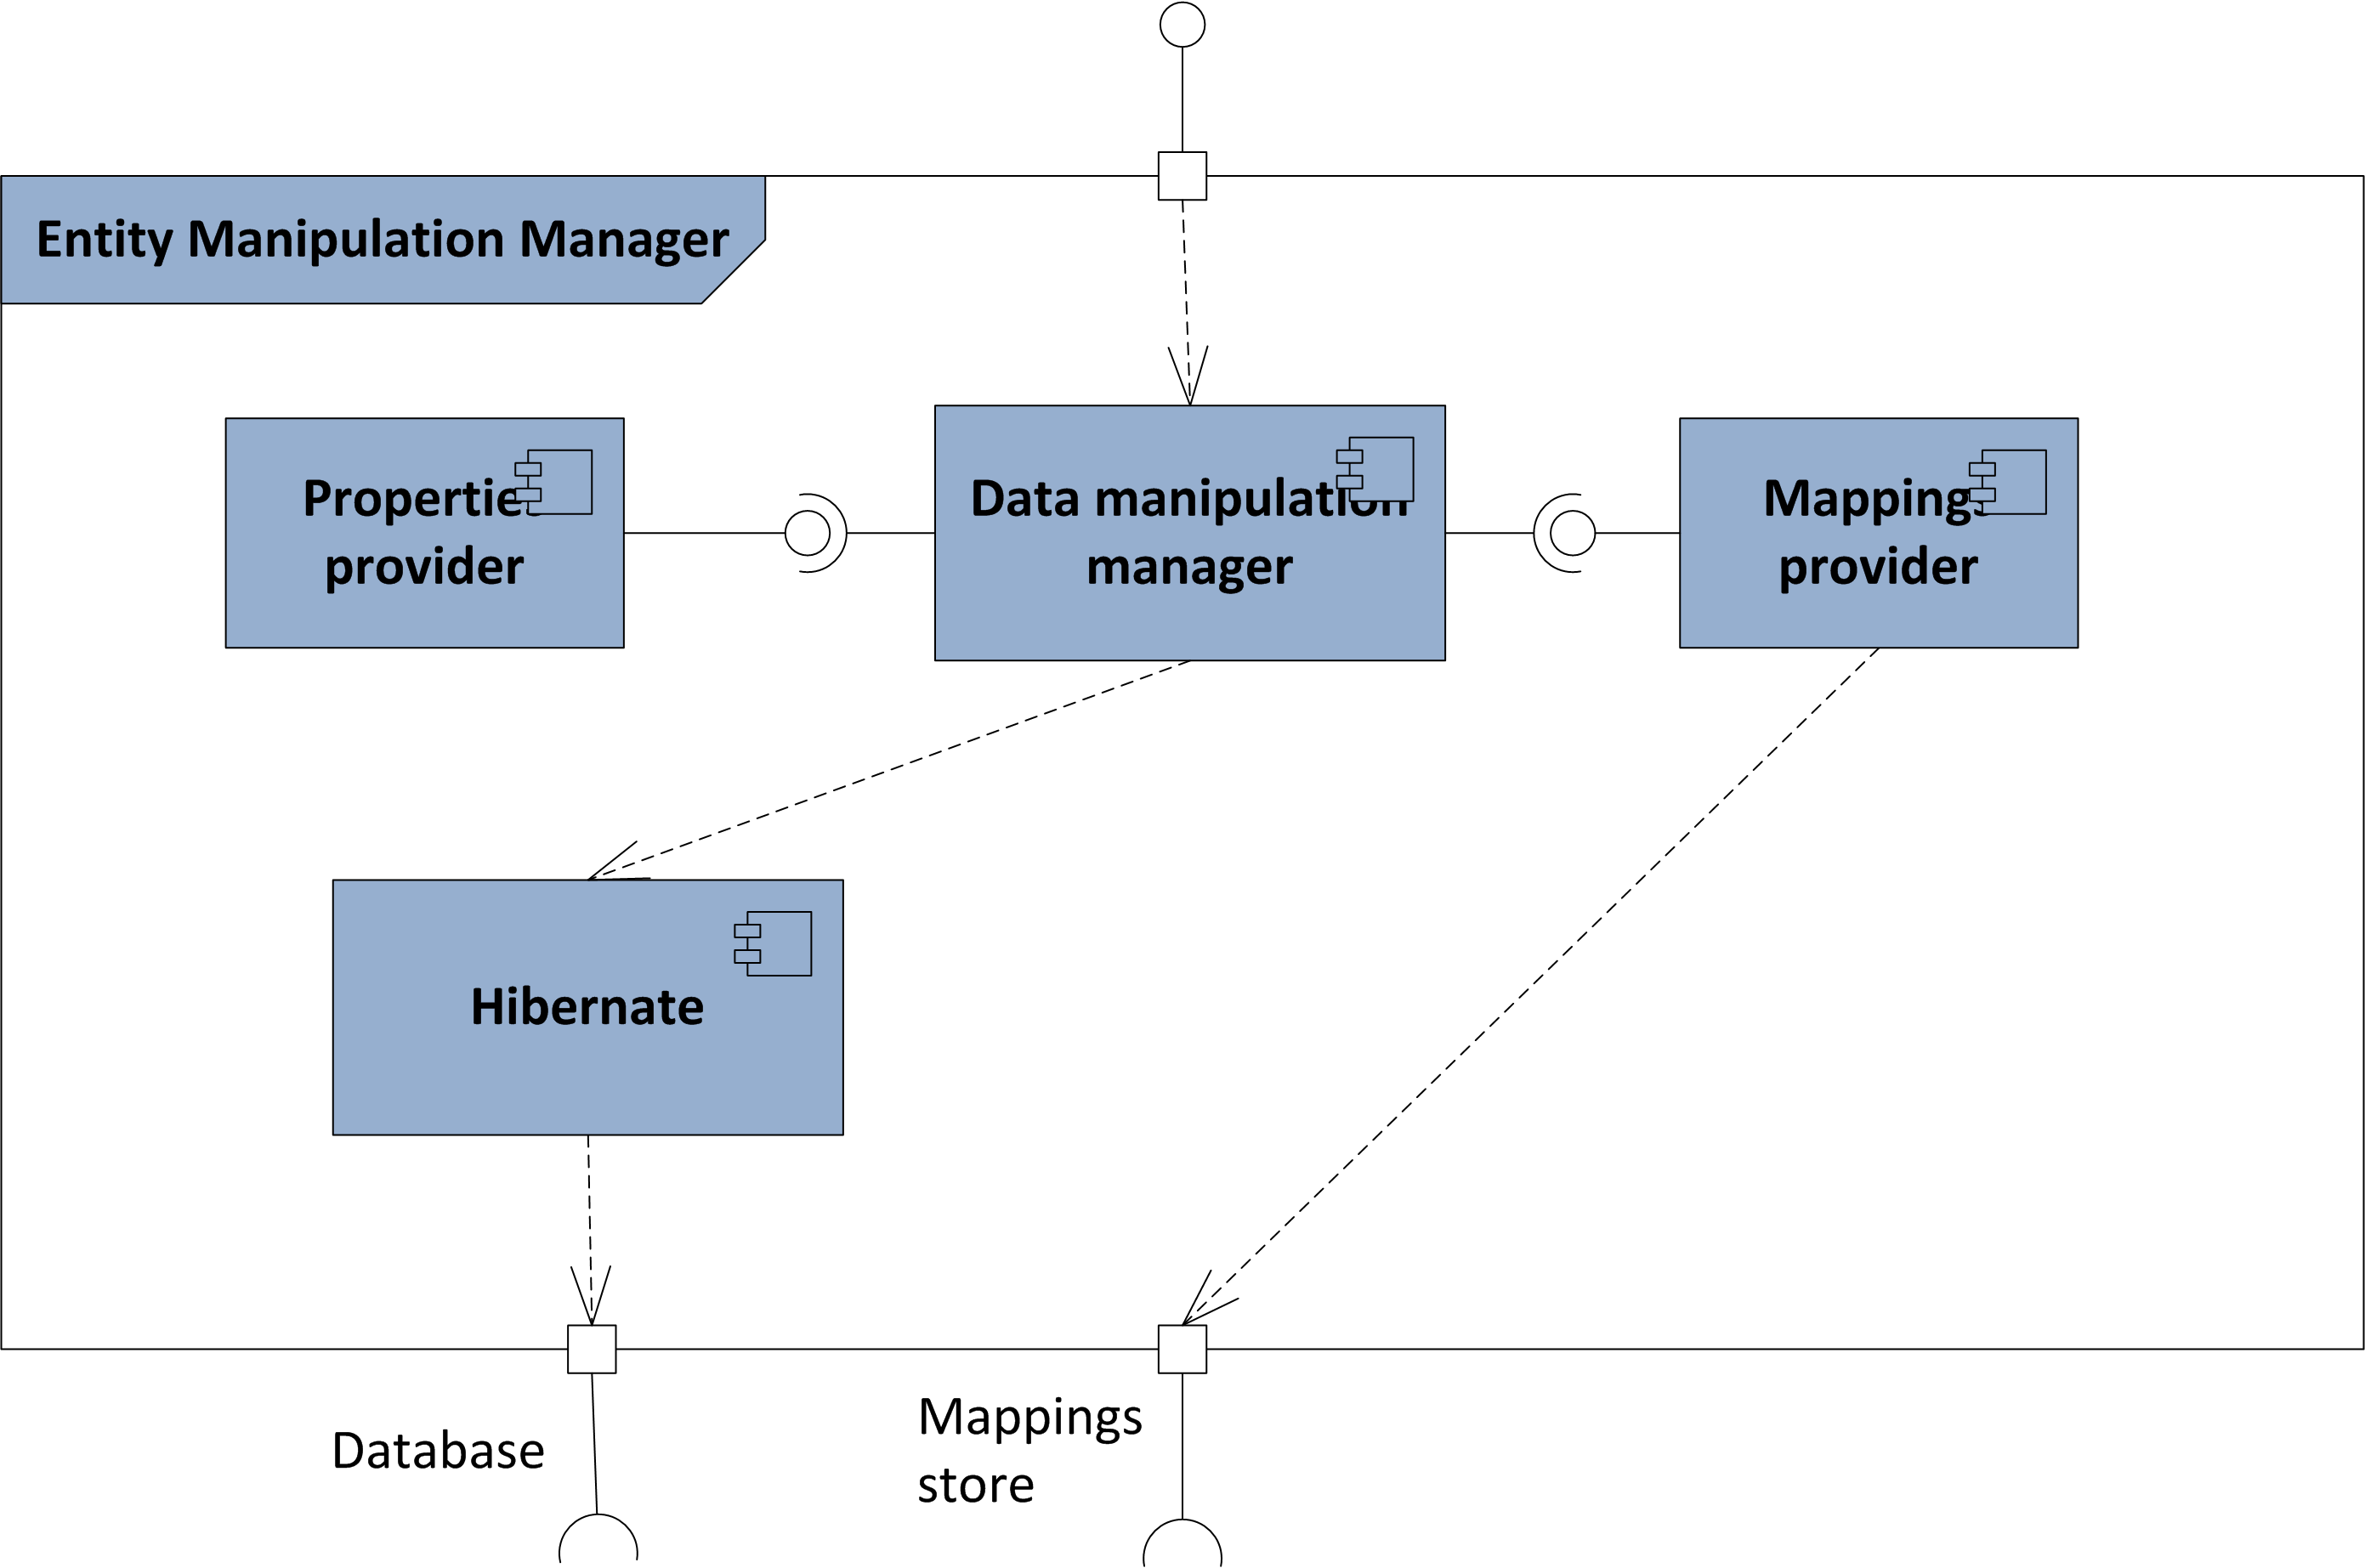
\includegraphics[scale=0.9]{storage/functional/func_manip.png}
  \caption{Functional decomposition of the Entities Manipulation Manager module}
  \label{fig:storageFuncManip}
\end{figure}

\subsection{Concurrency View}

This section describes the concurrency structure of the feature. We show how functional elements map to concurrency units (processes, process groups and threads) in order to clearly identify the parts of the system that can work concurrently. We also show how this parallel execution is coordinated and controlled.

Figure \ref{fig:storageConc} illustrates the concurrency organization. The main functionality of the system is situated in the U-Sem process group. All U-Sem processes including the storage processes operate concurrently. Workflow configuration and execution initiated by U-Sem clients and entity management by engineers can happen at the same time. This organization makes the solution flexible because if needed the \textit{Workflow engine} process can be replicated independently from the \textit{Administration}. However, this organization also introduces some problems that have to be solved.

\begin{figure}[h!]
  \centering
  	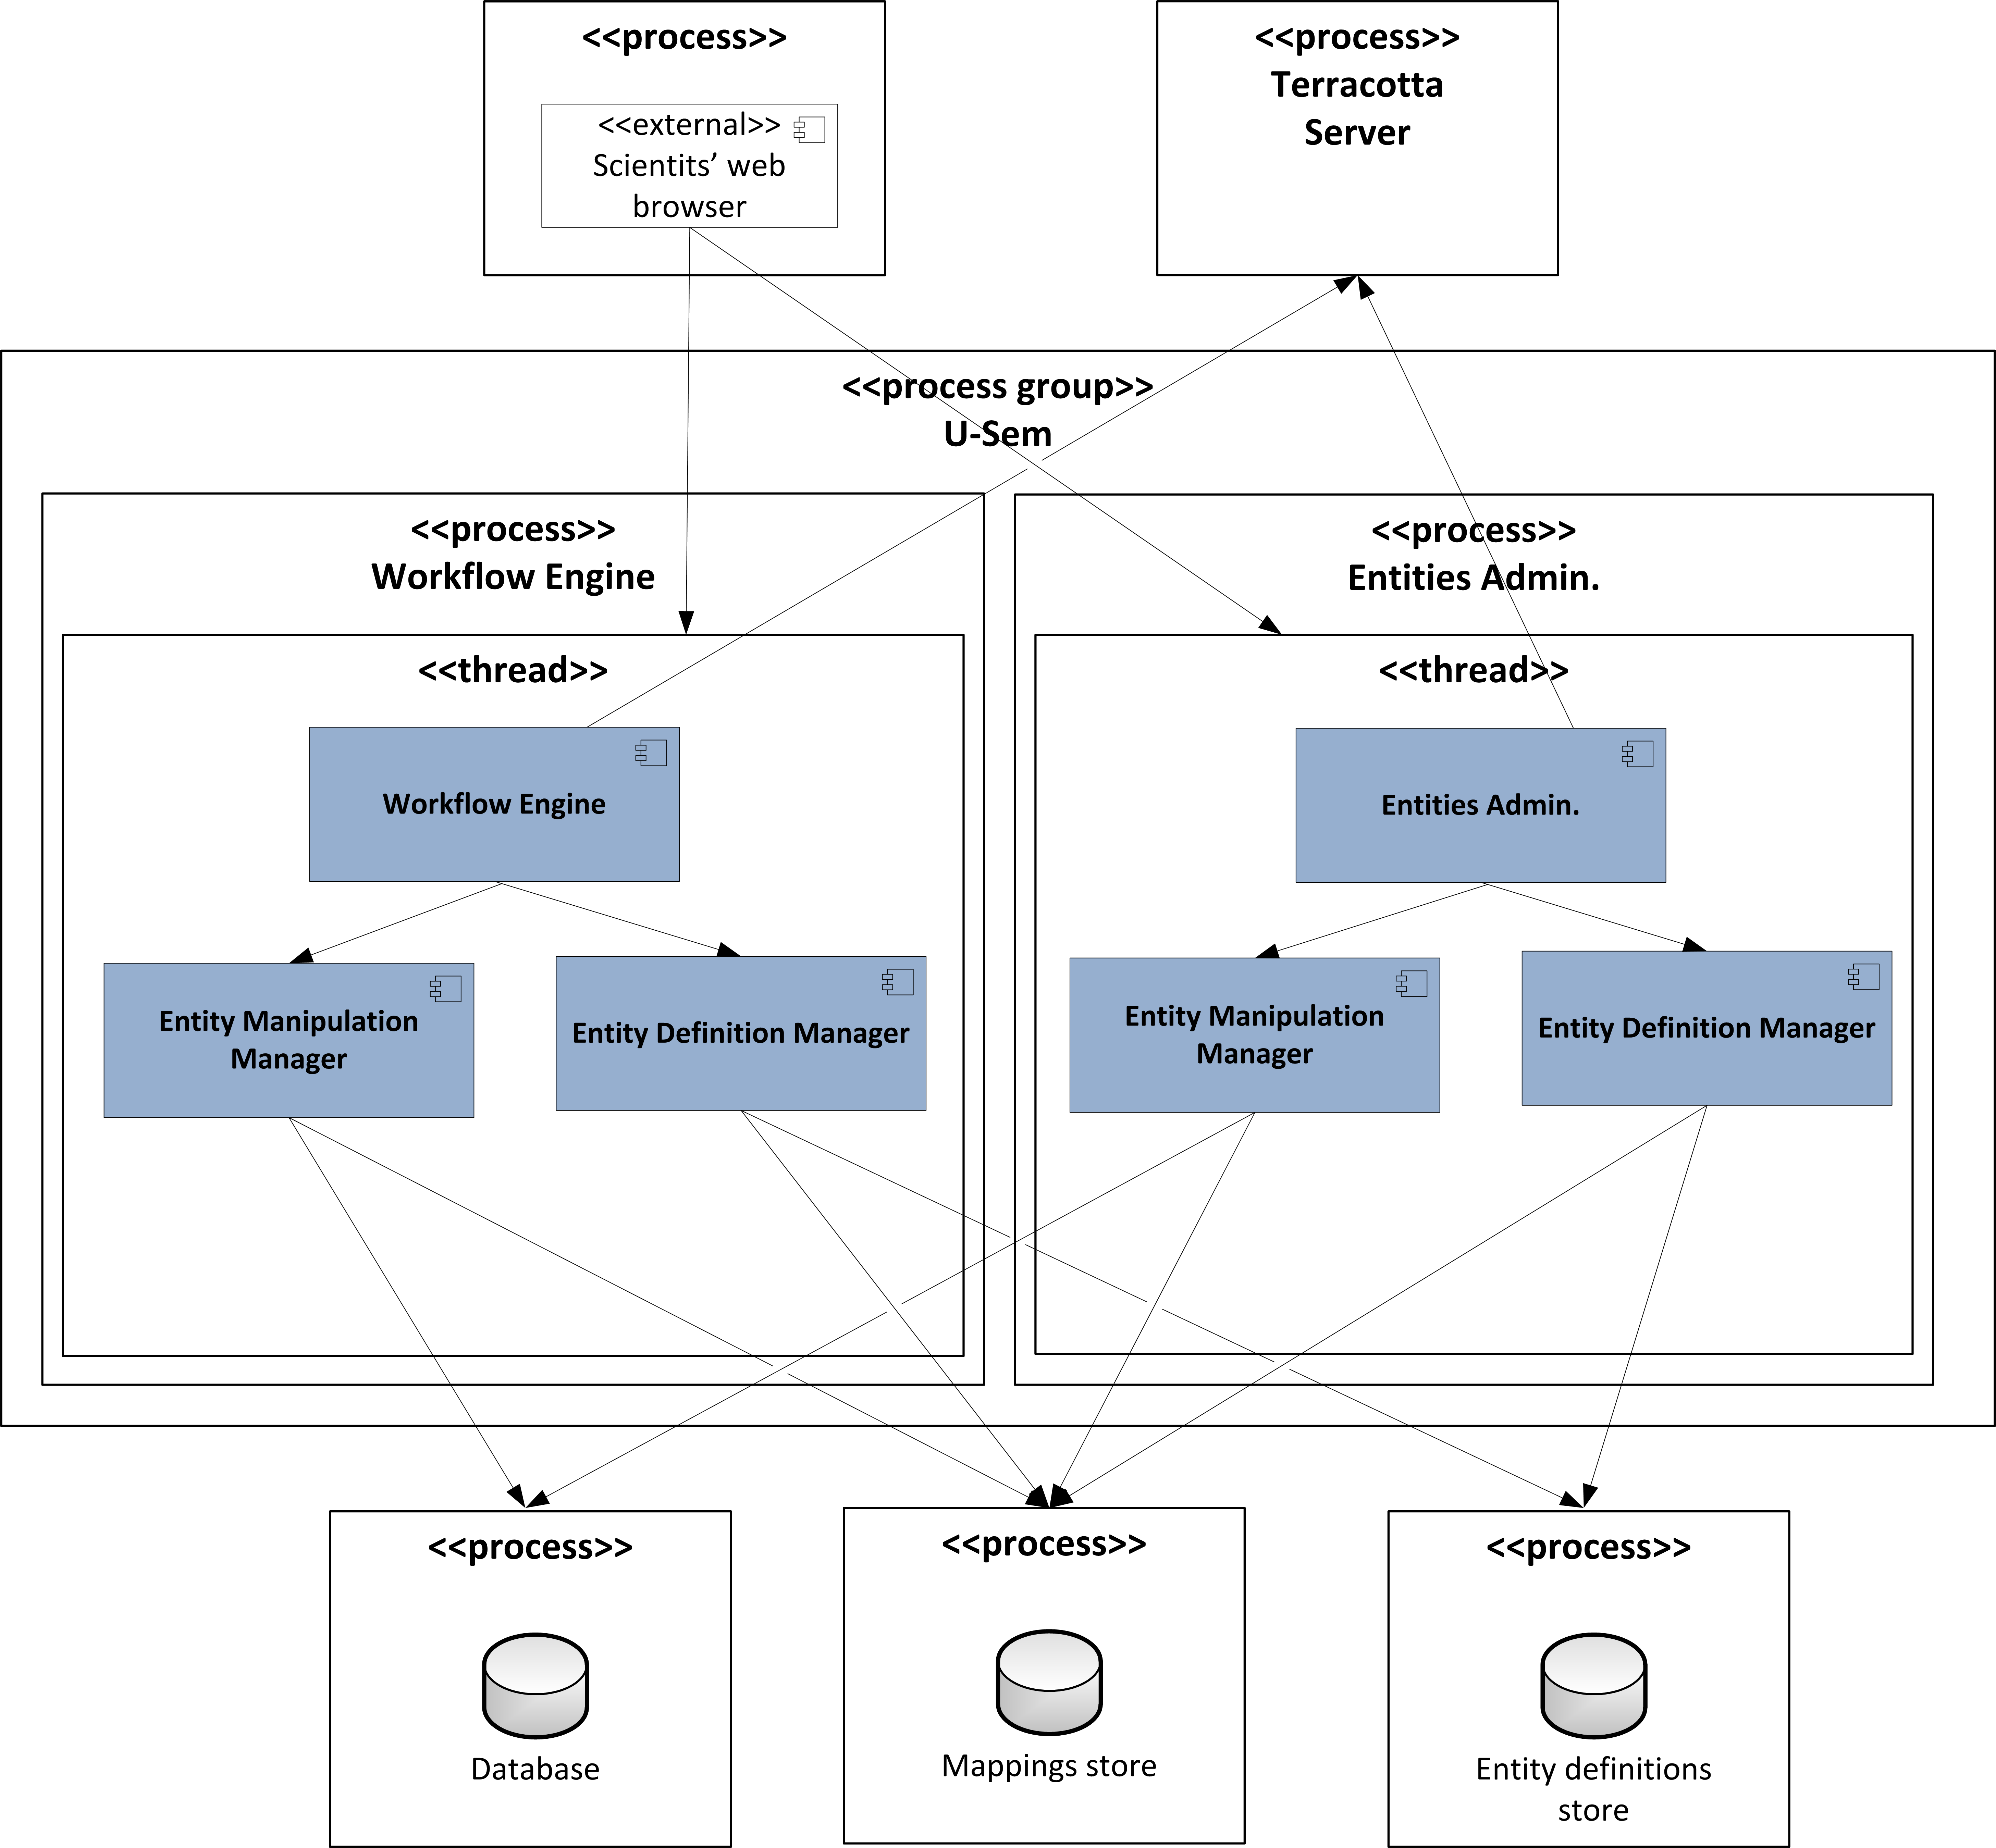
\includegraphics[scale=0.6]{storage/functional/concur.png}
  \caption{Diagram illustrating the concurrency model of the solution}
  \label{fig:storageConc}
\end{figure}

\subsubsection{Problems}
Firstly, if the workflow engine is the middle of execution and the structure of the database is changed, then the workflow may fail unexpectedly and cause problems that are hard to detect and reproduce. 

Secondly, every time the required resources for the data store interaction (entity definitions and mappings) are loaded the system has to make sure they are consistent with each other and also with the underling structure (schema) of the database. A problem can occur if the resources are loaded and modified simultaneously. It may happen that some of the files are loaded before the modification and others afterwards. This inconsistency can also lead to problems that are hard to detect and reproduce.

\subsubsection{Solution}

In order to solve the problems we propose a solution that is based on synchronization between the processes. The solution is based on the \textit{Reader-Writer Lock} idea \cite{lev2009scalable} discussed in Section \ref{sec:pluginConcur}. It maps to out problems as follows:

\begin{itemize}
	\item The shared resource is the combination of the entity definitions, mapping and the database schema.
	\item The workflow engine acts as reader of the shared resource.
	\item The entity administration acts as writer of the shared resource.
\end{itemize}

As a result, multiple workflows can be executed simultaneously but when a change to the entities is needed it is executed exclusively. Therefore, the workflow engine is protected against loading the resources while they are inconsistent. In order to implement this solution we follow the same approach introduced in Section \ref{sec:pluginConcur} and use the already introduced Terracotta server which is responsible to provide the locking mechanism. The workflow engine and entity admin. processes communicate with it in order to obtain the lock and use the resources.

\section{Implementation}
\label{sec:implStorage}

We implemented the proposed architecture in order to evaluate its applicability and capabilities. In this phase we basically implemented the system following the specification discussed in the previous section. Therefore, in this section we are discussing only on the most interesting parts of the implementation of the system.

\subsection{Entity definition storage}
We implemented the solution to store the entity definitions in the file system as xml files. The structure of these files is defined in a Document Type Definition (DTD) which is presented in Appendix \ref{cha:dtd}. It is based on the format provided in \cite{maro2011} for defining the RGL types of the input ports of RDF Gears components. We extended this format by adding additional elements corresponding to the entity's name, description, owner and the access control rules.

\subsection{Entities definition admin UI}
In order to implement the endpoints we used the jQuery UI\footnote{jQuery - http://jqueryui.com/} and Bootstrap\footnote{Bootstrap - http://twitter.github.com/bootstrap/} user interface technologies. The user interface consists of two main panels:
	\begin{itemize}
	
		\item \textit{Entities list} - Illustrated on Figure \ref{fig:storageEntityList}, this is the initial view exposed to the engineer. It provides a list of available entity definitions and enables engineers to create, update and delete entity definitions.
		
\begin{figure}[h!]
  \centering
  	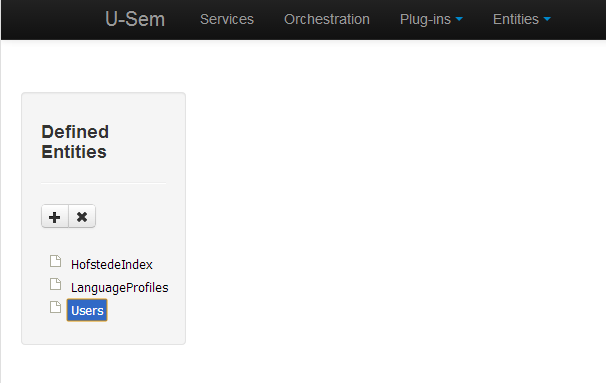
\includegraphics[scale=0.5]{storage/ui/entityList.png}
  \caption{User interface for entity definitions management}
  \label{fig:storageEntityList}
\end{figure}
		
		\item \textit{Entity manipulation panel} - The implementation also provides a panel that is responsible to automate the process of defining entities. Shown on Figure \ref{fig:storageEntityPanel}, this panel is used when an entity definition is created or updated.
		
\begin{figure}[h!]
  \centering
  	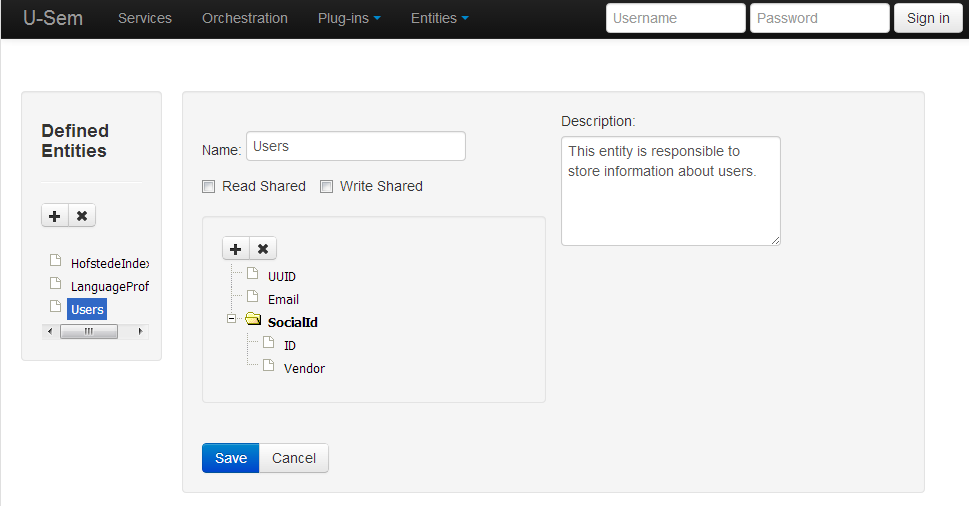
\includegraphics[scale=0.5]{storage/ui/entityPanel.png}
  \caption{User interface for constructing entity definitions}
  \label{fig:storageEntityPanel}
\end{figure}

	\end{itemize}


\subsection{RDF Gears workflow configuration}
We have also implemented two features that aim to benefit engineers when configuring workflows in RDF Gears.

The first feature concerns the \textit{Insert} component. According to the specification the engineer has to select an entity type that has to be stored and provide the corresponding data as inputs for the component. However, when selecting the entity type it is clear what are the inputs that will be required for the component because they have to correspond to the predefined entity structure. Therefore, instead of manually configuring the inputs of the component, the system reads the entity type definition and sets up all the required inputs automatically.

The second feature is the preview panel for entity types. It represents a small dialog panel in the user interface that can be opened every time the engineer defining workflows need to refer to the structure of an entity type. As shown on Figure \ref{fig:storageEntityPreview}, it presents the entity types in the form of a tree. This feature is particularly valuable when engineers have to write queries because they can easily refer to the entity types and therefore, they do not have to remember them. It is also likely to prevent mistakes connected to not reproducing the entity structure correctly in the queries.

\begin{figure}[h!]
  \centering
  	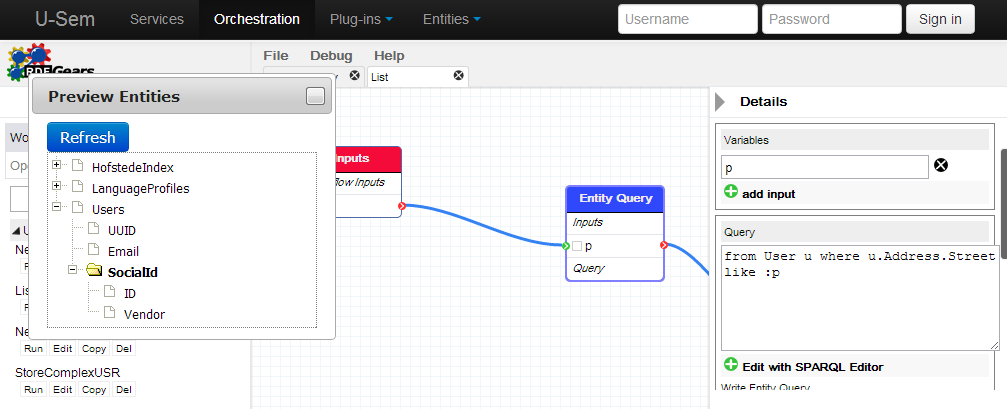
\includegraphics[scale=0.55]{storage/ui/entityPreview.png}
  \caption{User interface that provides a quick preview of the entity definitions}
  \label{fig:storageEntityPreview}
\end{figure}

\subsection{Extended workflow engine}

We incorporated the new workflow optimization and execution logic in RDF Gears by extending some of the classes involved in the process. In this way we kept the original classes almost intact. As a result, in case of a problem or if needed engineers can easily switch between the two implementations. We extended the following classes:

\begin{itemize}
	\item \textit{WorkflowNode} - the newly created class is responsible to act as a wrapper around the output node of the workflow. When executed it triggers the execution of not only the output node but also all the nodes with side effects defined in the workflow. The result of the execution is still the result of the execution of the output node. In this way we make sure that all nodes with side affects are executed as expected from the engineer. The already existing cashing mechanism discussed in Section \ref{sec:backRDFGears} ensures that each component is executed at most once which prevents any duplicate executions of components.
	
	\item \textit{WorkflowLoader} - the new child class extends the implementation in two directions. Firstly, when the workflow is compiled the resulted data structure contains not only the components needed for the execution of the output node but also the components with the side effects and their dependent components. Secondly, the output node implementations is replaced by the extended WorkflowNode, containing references to the output node and all nodes with side effects.
\end{itemize}


\section{Evaluation} 
\label{sec:evalStorage}

After successfully implementing the system, in this section we evaluate whether the system actually solves the problems identified in Section \ref{sec:problemDefStorage}. In order to do the evaluation we, first, performed an experiment presented in Appendix \ref{cha:transf} in which we reconstructed an already existing user modelling service using the new solution and identified the improvements it provides. Secondly, we asked engineers to use the new solution to implement real world user modelling services and asked them to comment on the problems the solution is designed to solve. The following is summary of the results of the experiment and the feedback which we received from the engineers:

\begin{itemize}

\item Implementing services that require data storage and retrieval no longer requires engineers to set up databases, implement special RDF Gears functional components and the tasks that accompany these processes. Engineers just have to configure the components provided by the solution so that they fit their needs. They reported that this improvement has significantly reduced the time and efforts they spend building such services. It has also reduced the amount of knowledge required so that new engineers can be trained faster.

\item Engineers reported that the solution has also enabled them to easily modify the structure of the data in their services when requirements change. This process is totally automated by the user interface of the solution and engineers no longer have to apply changes manually to the database and the source code of the RDF Gears components.

\item Engineers also reported that the solution has significantly facilitated collaboration between engineers on data level for two reasons. First, using the user interface of the system they can easily understand what are the structure and semantics of the data shared by other engineers without having to personally communicate it. And secondly, when sharing data they can control precisely who can execute what operations on the data. 

\item Finally, engineers reported that because of the extended RDF Gears notation they can now indicate their storage and retrieval components to have side effects. As a result, they no longer have to study the way services are executed by the workflow engine and worry whether their components will be executed correctly. 
	
\end{itemize}

Analysing this results we can conclude that we have solved the problems defining the Data Management feature and the designed and implemented system is capable of serving its intended purpose. As in most scientific works, however, there is still some place for improvement in this one as well. In next section we discuss possible directions for future work regarding the feature.

\section{Limitations and Future work}
\label{sec:limitsStorage}

In this section we identify the limitations of the proposed architecture and we also suggest approaches that can be used to overcome these limitation in the future. We have identified the following items:

\begin{itemize}
\item One of the limitations that our approach introduces is the way semantics of data are defined. Currently, engineers can describe them only in text form (in the description field). The way entities are described is left to the engineer, there are no automated mechanisms that manage or assist the process. Therefore, more sophisticated (formal) approach for describing semantics of entities might be beneficial.

\item The aim of this feature is to simplify the work with persistent data in U-Sem. However, introducing this abstraction over the storage functionality we have also reduced its flexibility to some extend. One of the side effects is the inflexibility in terms of transactions management. In the current situation engineers do not have any means to manage the database transactions and they are tied to the way the engine is configured. Currently, our research showed that this is not a problem but in future some engineers might need to have the power to control the transactions to the database. Therefore, introducing a mechanism that can enable that efficiently might be an interesting research topic.

\item Most of the data manipulation components (except for the "Insert" component) require engineers to provide JPQL queries. These queries can get quite complex and as a result engineers may make some mistakes when writing them. Currently, the solution does not provide any facilities that can validate these queries. Engineers realize their mistakes only when they try to execute the workflows and they fail. As a result, it may take a lot of time until they finally end up with the correct queries. Therefore, in future the system might be further improved by introducing functionality for auto-completion and validation of the JPQL queries.

\item Currently, the solution treats the RDF values as literals. However, these values sometimes may contain a lot of information that engineers might also like to query. SPARQL is the main language used for querying RDF data \cite{perez2006semantics} and therefore, extending the currently used JPQL language to support embedded SPARQL queries seems as a promising topic for future research.

\item Currently, the RDF Gears engine does not provide any guarantees for the order of the execution of branches. This is not a problem for components that do not have side effects. However, with the introduction of the new components that interact with the database developing a mechanism to control the execution order of branches within a workflow makes sense and might be a helpful future addition to the solution.

\item The system is currently targeted to be used mainly as a research tool and there are no requirements for supporting large number of users and high loads. However, if the system is to be used in such a demanding environment then it might be worth to investigate and if needed improve the performance, scalability and availability properties of the solution.


\end{itemize}

 

\chapter{\label{cha:conclusions}Conclusions and Future Work}

This chapter concludes our research. Section \ref{sec:concSumm} summarizes this thesis work and presents its main contributions. Section \ref{sec:concDisc} presents our conclusions on weather we have achieved the research goal. Finally Section \ref{sec:concFuture} discusses the possibilities for future work that we have identified.


\section{Summary}
\label{sec:concSumm}

In this thesis we presented the design and implementation of the U-Sem platform. Its main objective is to facilitate the everyday work of engineers building user modelling services based on the U-Sem idea. In order to achieve this objective, we first performed series of interviews in order to understand what are the tasks that engineers face every day and which of them require a lot of overhead work. Based on the results from the interviews we compiled a list of features which have to be implemented in order to achieve our goal. Due to the scope of this work we prioritized the features and designed and implemented only the ones that were indicated to bring the most improvement: the \textit{Plug-in Environment} and \textit{Data Management} features.

For the first feature we proposed and implemented a plug-in architecture based on OSGi which enables engineers to plug their custom RDF Gears function components and the related resources in the system on demand and without disturbing the work of other users of the system. We also proposed a mechanism for collaboration between engineers on component level using a plug-in repository. Finally, we designed and implemented a tool that facilitates the process of building plug-ins for the U-Sem platform and another tool that helps engineers to manage the dependencies between plug-ins.

For the second feature we proposed and implemented a solution integrated in U-Sem that is capable of supporting the data management tasks in U-Sem. Based on Hibernate, it enables engineers to store, manipulate and perform complex queries on RGL data structures without having to program custom components and be aware of how and where data is actually stored. We also propose mechanism which enables engineers to collaborate on data level. Finally, we integrate the two features to completely automate the installation and configuration of plug-ins that provide U-Sem services containing data management components.

\section{Conclusion}
\label{sec:concDisc}

The research goal of this thesis project was defined as:\\

\textit{Design and implement a platform that facilitates the work of engineers building user modelling services following the U-Sem approach}\\

In order to evaluate whether this goal is achieved we performed experiments and asked engineers to test the proposed solution in real world scenarios. The results presented in Sections \ref{sec:evalPlugin} and \ref{sec:evalStorage} confirmed that the solution actually facilitates the process of building U-Sem services by reducing the number of overhead tasks that engineers have to perform enabling them to focus on the core of their work. It saves them time, efforts and also reduces the amount of knowledge required in order to work with the system which also facilitates the process of training new engineers. The results also revealed that the solution additionally improves the performance of engineers by enabling them to collaborate effectively with each other. Therefore, we are confident that we have achieved the research goal and the proposed solution actually serves its purpose.

Additionally, apart from the U-Sem context, the developments in this work might be also beneficial for other fields. On one hand, the system can also be considered as an extension of RDF Gears. Therefore, all engineers using RDF Gears can potentially benefit from this work. On the other hand, we have designed the proposed features to be loosely coupled from the workflow engine by designing them as separate sub-systems providing access through APIs. Therefore, this sub-systems can be easily integrated in other workflow engines and this may also facilitate the work of their users.

\section{Future work}
\label{sec:concFuture}

The possibilities for future work that we have identified can be split into two categories. The first one covers how each of the implemented features can be improved in the future. We already discussed these in the Sections \ref{sec:evalPlugin} and \ref{sec:evalStorage} dedicated for each of the features. 

The second category concerns the U-Sem platform as a whole. In Section \ref{sec:features} we have identified the features providing which will facilitate the work of the engineers. Due to the scope of this work, however, we designed and implemented only the ones that were indicated to be most beneficial. Even though the rest might not provide so much benefits we believe that designing and implementing them can still bring some important improvements for the everyday work of the engineers.


\bibliographystyle{plain}
\bibliography{thesis}


\appendix
%dummy comment inserted by tex2lyx to ensure that this paragraph is not empty
\global\long\def\chaptername{Appendix}
 
\chapter{\label{cha:glossary}Glossary}

In this appendix we give an overview of frequently used terms and
abbreviations.
\begin{description}
\item [{foo:}] \ldots{} 
\item [{bar:}] \ldots{} 
\end{description}

 
\chapter{Requirements and Guidelines}

This chapter details some requirements and guidelines for MSc theses
submitted to the Software Engineering Research Group.


\section{Requirements}


\subsection{Layout}
\begin{itemize}
\item Your thesis should contain the formal title pages included in this
document (the page with the TU Delft logo and the one that contains
the abstract, student id and thesis committee). Usually there is also
a cover page containing the thesis title and the author (this document
has one) but this can be omitted if desired.
\item Base font should be an 11 point serif font (such as Times, New Century
Schoolbook or Computer Modern). Do not use sans-serif fonts such as
Arial or Helvetica. \textsl{Sans-serif type is intrinsically less
legible than seriffed type}
\item The final thesis and drafts submitted for reviewing should be printed
double-sided on A4 paper. 
\end{itemize}

\subsection{Content}
\begin{itemize}
\item The thesis should contain the following chapters: 

\begin{itemize}
\item Introduction.


Describes project context, goals and your research question(s). In
addition it contains an overview of how (the remainder of) your thesis
is structured.

\item One or (usually) more {}``main'' chapters.


Present your work, the experiments conducted, tool(s) developed, case
study performed, etc.

\item Overview of Related Work


Discusses scientific literature related to your work and describes
how those approaches differ from what you did.

\item Discussion/Evaluation/Reflection


What went well, what went less well, what can be improved?

\item Conclusions, Contributions, and (Recommendations for) Future Work
\item Bibliography
\end{itemize}
\end{itemize}

\subsection{Bibliography}
\begin{itemize}
\item Make sure you've included all required data such as journal, conference,
publisher, editor and page-numbers. When you're using \textsc{Bib}\TeX{},
this means that it won't complain when running \texttt{bibtex your-main-tex-file}.
\item Make sure you use proper bibliographic references. This especially
means that you should avoid references that \textbf{only} point at
a website and not at a printed publication.


For example, it's OK to add a URL with the entry for an article describing
a tool to point at its homepage, but it's not OK to just use the URL
and not mention the article. 

\end{itemize}

\section{Guidelines}
\begin{itemize}
\item The main chapters of a typical thesis contain approximately 50 pages.
\item A typical thesis contains approximately 50 bibliographic references.
\item Make sure your thesis structure is balanced (check this in the table
of contents).


Typically the main chapters should be of equal length. If they aren't,
you might want to revise your structure by merging or splitting some
chapters/sections.

In addition, the (sub)section hierarchies with the chapters should
typically be balanced and of similar depth. If one or more are much
deeper nested than others in the same chapter this generally signals
structuring problems.

\item Whenever you submit a draft of your thesis to your supervisor for
reviewing, make sure that you have checked the spelling and grammar.
Moreover, \emph{read it yourself at least once from start to end,
before submitting to your supervisor}.


\textbf{Your supervisor is not a spelling/grammar checker!}

\item Whenever you submit a second draft, include a short text which describes
the changes w.r.t. the previous version.
\end{itemize}

 
\chapter{\label{cha:priority}Prioritization questionnaire}

In this appendix we provide the questionnaire used for the prioritization of the requirements:\\

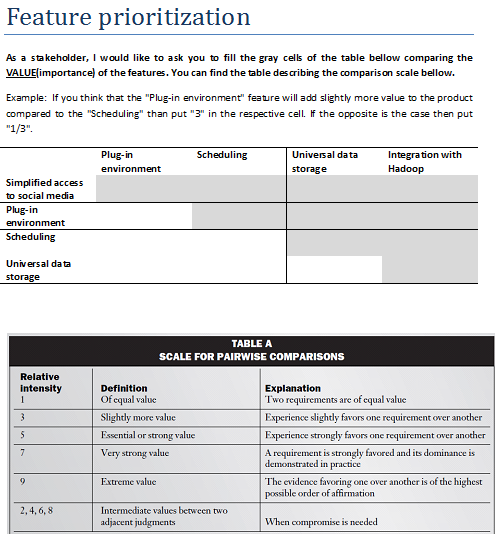
\includegraphics[scale=0.95]{apendix/prioritization/priority.png}

\end{document}
